\RequirePackage{fix-cm} % tamaños arbitrarios de la matemática CM (títulos de 13 pt)
\documentclass[11pt,letterpaper,oneside]{book} 

%% inyecta los paquetet
% Packages

\let\oldunderbar\underbar
\usepackage{blindtext}
\usepackage{amsbsy}
\usepackage{amssymb}
\usepackage{mathrsfs}
% rsfs escalable: los títulos de sección v5 son de 13 pt
\DeclareFontFamily{U}{rsfs}{\skewchar\font127 }
\DeclareFontShape{U}{rsfs}{m}{n}{<-6> rsfs5 <6-8> rsfs7 <8-> rsfs10}{}
\usepackage{amsmath} 
% Identidad UAM (Acuerdo 06/2012, numeral 4.1): Helvetica Neue en todas sus
% variantes como tipografía primaria del material impreso. Exige lualatex.
\usepackage{fontspec}
\setmainfont{HelveticaNeue}[
  BoldFont       = {HelveticaNeue-Bold},
  ItalicFont     = {HelveticaNeue-Italic},
  BoldItalicFont = {HelveticaNeue-BoldItalic}
]
\setsansfont{HelveticaNeue}[
  BoldFont       = {HelveticaNeue-Bold},
  ItalicFont     = {HelveticaNeue-Italic},
  BoldItalicFont = {HelveticaNeue-BoldItalic}
]
\setmonofont{Menlo}[Scale=MatchLowercase]
\newfontfamily\uamcondensed{HelveticaNeue-CondensedBold}
\usepackage[margin=2.6cm, headsep=14pt, footskip=30pt]{geometry} % v5 UAM Dato: medida de línea 16,39 cm
\usepackage[english,spanish,es-lcroman]{babel}
\spanishdecimal{.}
\usepackage{graphicx}
\usepackage{setspace}
\usepackage[hidelinks]{hyperref}
\usepackage{fancyhdr}

\usepackage{import}
\usepackage{makecell}
\usepackage{ragged2e}
\usepackage{csquotes}
\usepackage{caption}
\usepackage{subfig}
\usepackage{color}
\usepackage{siunitx}
\usepackage{tikz}
\usepackage{pgfplots}
\pgfplotsset{compat=1.18}
  \usetikzlibrary{babel}
  \usetikzlibrary{shapes.geometric, arrows}
  \usetikzlibrary{arrows,positioning,patterns,decorations.pathmorphing}
\usepackage{circuitikz}
\usepackage{etoolbox}
\usepackage[
backend=biber,
style=ieee,
sorting=ynt
]{biblatex}
\addbibresource{bibliography/referencias.bib}
\usepackage{tabularx}
\usepackage[numbib]{tocbibind}
\usepackage{multicol}
\usepackage{pgfgantt}
\usepackage{enumitem}
\usepackage{float} 
\usepackage{wrapfig}
\usepackage{smartdiagram}
\usepackage{lipsum}
\usepackage{ifthen}
\usepackage{comment}
\usepackage{microtype}
\usepackage{placeins}
%% ruta de las imagenes
\graphicspath{ {images/} }

\makeatletter
  \renewcommand{\author}[2]{\gdef\insauthor{#2}\gdef\@author{#2}\gdef\insheadauthor{#1}\gdef\@author{#1}}
  \newcommand{\programme}[1]{\gdef\insprog{#1}\gdef\@programme{#1}}
  \renewcommand{\title}[2][1]{\gdef\institle{#2}\gdef\@title{#2}\gdef\insheadtitle{#2}\gdef\@title{\tiny#2}\gdef\insversion{\othertwodigits#1}\gdef\@title{#1}}
  \newcommand{\supervisor}[2]{\gdef\inssupervisor{#1}\gdef\@supervisor{#1}\gdef\insadscription{#2}\gdef\@supervisor{#2}}
  \newcommand{\cosupervisor}[2]{\gdef\inscosupervisor{#1}\gdef\@cosupervisor{#1}\gdef\inscoadscription{#2}\gdef\@cosupervisor{#2}}
  \newcommand{\Date}{\leavevmode\hbox{\twodigits\day/\twodigits\month/\the\year}}
  \def\twodigits#1{\ifnum#1<10 0\fi\the#1}
  \def\othertwodigits#1{\ifnum#1<10 0\fi#1}
\makeatother

% Identidad v5 "UAM Dato": paleta, títulos, cabecera/pie, índice y componentes.
%══════════════════════════════════════════════════════
% Identidad v5 "UAM Dato" adaptada a la tesis (clase book)
%
% Origen: ~/uam-identidad-kit/UAMDato/plantilla_dato.tex (clase article).
% Paleta, escala tipográfica (0.55 frente al deck), kicker, chips,
% cabecera/pie y componentes se copian sin cambio. Lo único que se
% adapta es el nivel de los títulos:
%   plantilla \section     -> tesis \chapter  (kicker + chip + filete)
%   plantilla \subsection  -> tesis \section
%   plantilla \subsubsection -> tesis \subsection
% Compila con lualatex (ver .latexmkrc); fontspec ya se carga en
% packages/packages.tex con las caras de Helvetica Neue por nombre PostScript.
%══════════════════════════════════════════════════════

\usepackage{titlesec,titletoc}
\usepackage{booktabs,array,multirow,colortbl,xltabular}
\usepackage{parskip}
\usepackage[most]{tcolorbox}
\tcbuselibrary{skins,breakable,raster}

% Interlineado 1.4x, el mismo del cuerpo del deck (28pt sobre 20pt).
\linespread{1.13}

%──────────────────────────────────────────────────────
% Paleta --- idéntica al deck; verificada contra el Acuerdo 06/2012.
%──────────────────────────────────────────────────────
\definecolor{uamred}{RGB}{205,3,46}        % Pantone 186 C, Azcapotzalco, numeral 5.3 p.49
\definecolor{uamblue}{RGB}{28,28,28}       % tinta de cuerpo; #000000 se reserva al emblema (numeral 2.3)
\definecolor{uamgray}{RGB}{100,100,100}
\definecolor{uamlightgray}{RGB}{244,244,244}
\definecolor{hairline}{RGB}{222,222,222}
\definecolor{darktext}{HTML}{EDEDED}
\definecolor{darkmeta}{HTML}{9A9A9A}
\definecolor{darkrule}{HTML}{3A3A3A}
\arrayrulecolor{hairline}
\AtBeginDocument{\color{uamblue}}

% Emblemas copiados del kit a images/titlepage/ para que la tesis no
% dependa de rutas fuera del proyecto.
\newcommand{\assetPie}{titlepage/logo_footer.png}
% logo_uam_reconstruido.pdf no existe en disco; se usa logo_uam.pdf
% como respaldo temporal para poder compilar (ver aviso en el reporte).
\newcommand{\assetPortada}{titlepage/logo_uam.pdf}

%══════════════════════════════════════════════════════
% Escala tipográfica (LetterSpace es porcentaje del em: 8 = 0.08 em)
%══════════════════════════════════════════════════════
\newcommand{\escKicker}{\bfseries\fontsize{8}{10}\selectfont
  \addfontfeature{LetterSpace=8}}
\newcommand{\escTitulo}{\bfseries\fontsize{28}{32}\selectfont}
\newcommand{\escSeccion}{\bfseries\fontsize{24}{28}\selectfont}
\newcommand{\escSubtitulo}{\fontsize{12}{16}\selectfont}
\newcommand{\escMeta}{\ttfamily\fontsize{8}{11}\selectfont}

\newcommand{\kicker}[1]{{\escKicker\color{uamred}\MakeUppercase{#1}}\par\vspace{4pt}}
\newcommand{\kickergris}[1]{{\escKicker\color{uamgray}\MakeUppercase{#1}}\par\vspace{4pt}}

%──────────────────────────────────────────────────────
% Chips circulares (la fuente se fija antes del tikzpicture para que
% `em` sea el de la letra del chip).
%──────────────────────────────────────────────────────
\newcommand{\chipgen}[3]{%
  {\bfseries\fontsize{#1}{#1}\selectfont
   \tikz[baseline=(chipnodo.base)]{%
     \node[circle, fill=#2, inner sep=0pt, minimum size=2.3em,
       text height=0.68em, text depth=0pt, align=center,
       text=white, font=\bfseries] (chipnodo) {#3};}}%
}
\newcommand{\seccionchip}[1]{\chipgen{7}{uamred}{#1}}
\newcommand{\chiplg}[1]{\chipgen{11}{uamred}{#1}}
\newcommand{\chipgris}[1]{\chipgen{7}{uamgray}{#1}}
\newcommand{\puntorojo}{\raisebox{0.22em}{\tikz\fill[uamred] (0,0) circle (2.1pt);}}
\newcommand{\puntogris}{\raisebox{0.22em}{\tikz\fill[uamgray] (0,0) circle (2.1pt);}}
\newcommand{\puntohueco}{\raisebox{0.22em}{\tikz\draw[uamgray,line width=0.5pt] (0,0) circle (2.1pt);}}

%──────────────────────────────────────────────────────
% Capítulos: kicker + chip + título en caja normal + filete, en un solo
% bloque [display] para que un salto de página no los separe. El kicker
% por omisión es "Capítulo" / "Anexo"; \bloque{...} antes de \chapter
% lo sustituye por el nombre del bloque al que pertenece.
%──────────────────────────────────────────────────────
\newcommand{\kickervacio}{}
\newcommand{\kickeractual}{}
\newcommand{\bloque}[1]{\gdef\kickeractual{#1}}
\titleformat{\chapter}[display]
  {\color{uamblue}}
  {{\escKicker\color{uamred}%
     \ifx\kickeractual\kickervacio\MakeUppercase{\chaptertitlename}%
     \else\MakeUppercase{\kickeractual}\fi}}
  {5pt}
  {\escSeccion\seccionchip{\thechapter}\hspace{0.5em}}
  [\vspace{5pt}{\color{hairline}\hrule height 0.5pt}\vspace{6pt}%
   \global\let\kickeractual\kickervacio]
% \chapter* no actualiza la marca de la cabecera: \marcasinnumero la fija
% con el propio título (titlesec se lo pasa como argumento).
\newcommand{\marcasinnumero}[1]{#1\markboth{#1}{}}
\titleformat{name=\chapter,numberless}[display]
  {\color{uamblue}}
  {}
  {0pt}
  {\escSeccion\marcasinnumero}
  [\vspace{5pt}{\color{hairline}\hrule height 0.5pt}\vspace{6pt}]
% Cada capítulo abre página nueva (book): sin espacio superior extra.
\titlespacing*{\chapter}{0pt}{0pt}{1.6ex}

\titleformat{\section}
  {\bfseries\fontsize{13}{17}\selectfont\color{uamblue}}
  {\textcolor{uamred}{\thesection}}
  {0.5em}{}
\titlespacing*{\section}{0pt}{3ex plus .5ex}{0.7ex}

\titleformat{\subsection}
  {\escKicker\color{uamgray}}
  {\thesubsection}{0.6em}{\MakeUppercase}
\titlespacing*{\subsection}{0pt}{2.4ex plus .3ex}{0.5ex}

%──────────────────────────────────────────────────────
% Cabecera y pie: filete hairline arriba y abajo, emblema y folio en
% Menlo 8 pt. \doctag es el identificador corto del documento.
%──────────────────────────────────────────────────────
\newcommand{\doctag}{ICR \textperiodcentered{} MCIE \textperiodcentered{} UAM-A}
\renewcommand{\chaptermark}[1]{\markboth{#1}{}}
\renewcommand{\sectionmark}[1]{}
\newcommand{\logopie}{\raisebox{-0.09cm}{\includegraphics[height=0.32cm]{\assetPie}}}

\pagestyle{fancy}\fancyhf{}
\fancyhead[L]{\escMeta\color{uamgray}\doctag}
\fancyhead[R]{\escMeta\color{uamgray}\nouppercase{\leftmark}}
\fancyfoot[L]{\logopie}
\fancyfoot[R]{\escMeta\color{uamgray}\thepage}
\renewcommand{\headrulewidth}{0.5pt}
\renewcommand{\footrulewidth}{0.5pt}
\renewcommand{\headrule}{{\color{hairline}\hrule width\headwidth height 0.5pt}}
\renewcommand{\footrule}{\vspace{-10pt}{\color{hairline}\hrule width\headwidth height 0.5pt}\vspace{10pt}}
\setlength{\headheight}{16pt}
% Las páginas de inicio de capítulo (estilo plain en book) llevan la misma caja.
\fancypagestyle{plain}{}

%──────────────────────────────────────────────────────
% Índice
%──────────────────────────────────────────────────────
\titlecontents{chapter}[0pt]
  {\addvspace{9pt}\bfseries\color{uamblue}}
  {\seccionchip{\thecontentslabel}\hspace{0.6em}}
  {}
  {\normalfont\color{uamgray}\;\titlerule*[0.4pc]{.}\;\contentspage}
\titlecontents{section}[1.7em]
  {\normalfont\small\color{uamblue}}
  {\textcolor{uamred}{\thecontentslabel}\hspace{0.5em}}
  {}
  {\normalfont\small\color{uamgray}\;\titlerule*[0.4pc]{.}\;\contentspage}
\titlecontents{subsection}[4.2em]
  {\normalfont\small\color{uamgray}}
  {\thecontentslabel\hspace{0.5em}}
  {}
  {\;\titlerule*[0.4pc]{.}\;\contentspage}
\titlecontents{figure}[0pt]
  {\normalfont\small\color{uamblue}}
  {\textcolor{uamred}{\thecontentslabel}\hspace{0.8em}}
  {}
  {\normalfont\small\color{uamgray}\;\titlerule*[0.4pc]{.}\;\contentspage}
\titlecontents{table}[0pt]
  {\normalfont\small\color{uamblue}}
  {\textcolor{uamred}{\thecontentslabel}\hspace{0.8em}}
  {}
  {\normalfont\small\color{uamgray}\;\titlerule*[0.4pc]{.}\;\contentspage}

\captionsetup{font=small,labelfont=bf,labelsep=period}

%══════════════════════════════════════════════════════
% Componentes del sistema (disponibles para el texto)
%   \dato / \datochico / \datohero dentro de datorow
%   \tarjeta / \tarjetasdos / \tarjetastres
%   lista filas con \filaitem{}{}
%   tablaA / tablaB con \thA / \thB / \celdaacento / \celdameta
% En la tesis la columna Y es centrada (preamble/macros.tex); en las
% tablas de este sistema usa Z, la X alineada a la izquierda.
%══════════════════════════════════════════════════════
\newcommand{\datoetiqueta}[1]{%
  {\color{uamgray}\bfseries\fontsize{8}{11}\selectfont
   \addfontfeature{LetterSpace=7}\MakeUppercase{#1}}}
\newcommand{\dato}[3][uamblue]{%
  \begin{minipage}[t]{\linewidth}\centering
    {\color{#1}\bfseries\fontsize{34}{34}\selectfont #2}\par\vspace{7pt}
    \datoetiqueta{#3}\par
  \end{minipage}%
}
\newcommand{\datochico}[3][uamblue]{%
  \begin{minipage}[t]{\linewidth}\centering
    {\color{#1}\bfseries\fontsize{23}{25}\selectfont #2}\par\vspace{6pt}
    \datoetiqueta{#3}\par
  \end{minipage}%
}
\newcommand{\datohero}[3][uamred]{%
  \par\vspace{6pt}
  \begin{minipage}[t]{\linewidth}\centering
    {\color{#1}\bfseries\fontsize{80}{80}\selectfont #2}\par\vspace{10pt}
    \datoetiqueta{#3}\par
  \end{minipage}\par\vspace{6pt}%
}
\newcolumntype{H}{!{\color{hairline}\vrule width 0.5pt}}
\newenvironment{datorow}{%
  \par\medskip\noindent{\color{hairline}\hrule height 0.5pt}\par\vspace{11pt}
}{%
  \par\vspace{9pt}{\color{hairline}\hrule height 0.5pt}\par\medskip
}

\newcommand{\tarjetaopts}{breakable}
\newtcolorbox{tarjetabase}[1][]{enhanced,
  colback=uamlightgray, colframe=uamlightgray, boxrule=0pt,
  sharp corners, left=12pt, right=12pt, top=11pt, bottom=11pt, #1}
\newcommand{\tarjeta}[3][]{%
  \begin{tarjetabase}[\tarjetaopts]
    \setlength{\parskip}{0pt}%
    \noindent\begin{minipage}[t]{\linewidth}
      \ifx\relax#1\relax\puntogris\else\chiplg{#1}\fi\hspace{7pt}%
      {\raggedright\bfseries\fontsize{10.5}{13}\selectfont\color{uamblue}#2\par}
      \vspace{5pt}
      {\raggedright\fontsize{8.5}{11.5}\selectfont\color{uamgray}#3\par}
    \end{minipage}
  \end{tarjetabase}%
}
\newcommand{\tarjetasdos}[6]{%
  \par\renewcommand{\tarjetaopts}{}%
  \begin{tcbraster}[raster columns=2, raster equal height,
    raster column skip=5mm, raster left skip=0pt, raster right skip=0pt,
    raster force size=false]
    \tarjeta[#1]{#2}{#3}
    \tarjeta[#4]{#5}{#6}
  \end{tcbraster}%
  \renewcommand{\tarjetaopts}{breakable}%
}
\newcommand{\tarjetastres}[9]{%
  \par\renewcommand{\tarjetaopts}{}%
  \begin{tcbraster}[raster columns=3, raster equal height,
    raster column skip=5mm, raster left skip=0pt, raster right skip=0pt,
    raster force size=false]
    \tarjeta[#1]{#2}{#3}
    \tarjeta[#4]{#5}{#6}
    \tarjeta[#7]{#8}{#9}
  \end{tcbraster}%
  \renewcommand{\tarjetaopts}{breakable}%
}

% Viñetas del texto corrido: el punto del sistema en lugar del cuadro que
% pone babel en español (gris, para no sumar acentos rojos).
\setlist[itemize,1]{label=\puntogris}
\setlist[itemize,2]{label=\puntohueco}

\newlist{filas}{itemize}{1}
\setlist[filas]{label=\puntohueco, leftmargin=1.5em, itemsep=9pt,
  parsep=0pt, topsep=7pt}
\newcommand{\filaitem}[2]{%
  \item {\bfseries\fontsize{11}{14}\selectfont\color{uamblue}#1}\par
        \vspace{2pt}{\fontsize{9}{12}\selectfont\color{uamgray}#2}}

\newcommand{\thA}[1]{\cellcolor{uamlightgray}%
  \raisebox{0.22\baselineskip}[0pt][0pt]{%
  {\bfseries\fontsize{8}{10}\selectfont\addfontfeature{LetterSpace=4}%
   \color{uamblue}\MakeUppercase{#1}}}}
\newcommand{\thB}[1]{%
  {\bfseries\fontsize{8}{10}\selectfont\addfontfeature{LetterSpace=4}%
   \color{uamblue}\MakeUppercase{#1}}}
\newcommand{\celdaacento}[1]{{\bfseries\color{uamred}#1}}
\makeatletter
\newcommand{\celdameta}[1]{{\ttfamily\fontsize{8}{\f@baselineskip}\selectfont
  \color{uamgray}#1}}
\makeatother
\newenvironment{tablaA}{%
  \par\medskip
  \setlength{\arrayrulewidth}{0.5pt}\arrayrulecolor{hairline}%
  \renewcommand{\arraystretch}{1.45}%
  \fontsize{10}{13.2}\selectfont
}{\par\medskip}
\newenvironment{tablaB}{%
  \par\medskip
  \setlength{\arrayrulewidth}{0.5pt}\arrayrulecolor{hairline}%
  \renewcommand{\arraystretch}{1.5}%
  \fontsize{9}{11.5}\selectfont
}{\par\medskip}
\newcommand{\reglaB}{\noalign{{\color{uamblue}\hrule height 0.6pt}}}
\newcolumntype{Z}{>{\raggedright\arraybackslash}X}


\makeatletter
	\def\tableofcontents{\chapter{Contenido}\vskip1cm\@starttoc{toc}}
	\def\listoffigures{\chapter{Índice de Figuras}\@starttoc{lof}}
	\def\listoftables{\chapter{Índice de Tablas}\@starttoc{lot}}
    \def\thebibliography{\chapter{Referencias}} 	
\makeatother

\renewcommand{\appendixname}{Anexo}

\setlength{\parindent}{0pt}
%%%%%%%%%%%%%%%%%%%%%%%%%%%%%%%%%%%%%%%%%%%%%
%
%       Dedication environment
\newenvironment{dedication}
{
   \cleardoublepage
   \thispagestyle{empty}
   \vspace*{\stretch{1}}
   \hfill\begin{minipage}[t]{0.66\textwidth}
   \raggedright
}%
{
   \end{minipage}
   \vspace*{\stretch{3}}
   \clearpage
}
%%%%%%%%%%%%%%%%%%%%%%%%%%%%%%%%%%%%%%%%%%%%%
%
      %Glossary
%\makeglossary

% Helvetica Neue es más ancha que Computer Modern: holgura para evitar renglones desbordados
\setlength{\emergencystretch}{3em}

%%%%%%%%%%%%%%%%%%%%%%%%%%%%%%%%%%%%%%%%%%%%%%
%                PhD Thesis                  %
%    Mathematical enviornment definitions    %
%           C.S. Lopez-Monsalvo              %
%        University of Southampton           %
%                  2011                      %
%%%%%%%%%%%%%%%%%%%%%%%%%%%%%%%%%%%%%%%%%%%%%%

	\newcommand{\ncd}{\newcommand}

	\ncd{\mrm}{\mathrm}
	\newcommand{\beq}{\begin{equation}}
        \newcommand{\eeq}{\end{equation}}
	\ncd{\glo}[2]{\glossary{name = {#1}, description = {#2}}}
	\ncd{\nn}{\nonumber}

	\ncd{\PM}{BLDC}
	\ncd{\bb}[1]{\boldsymbol{#1}}
	\ncd{\vv}[1]{\mathbf{#1}}
	\newcommand{\lrp}[1]{\left(#1\right)}
        \newcommand{\lrb}[1]{\left[#1\right]}
	\ncd{\ode}[3][{}]{\frac{\text{d}^{#1}#2}{\text{d}#3^{#1}}}
	\ncd{\diff}[1]{\text{d}#1}
	\ncd{\req}[1]{(\ref{#1})}
	\ncd{\LL}{\mathscr{L}}
	\ncd{\fth}{\lrp{\theta_r}}
	
	\newcolumntype{Y}{>{\centering\arraybackslash}X}
	\renewcommand\tabularxcolumn[1]{m{#1}}
	
	\addto{\captionsspanish}{\renewcommand{\bibname}{Referencias}}
	\addto{\captionsspanish}{\renewcommand{\tablename}{Tabla}}
	\addto{\captionsspanish}{\renewcommand{\appendixname}{Anexo}}
	
    \newcommand{\signature}{%
      \hfill
      \begin{minipage}{\textwidth}     
          \vspace*{2\baselineskip}
          \begin{center}
            \parbox{0.4\textwidth}{
            \centering
            {\footnotesize Ing. \insauthor}\\   
            \vspace*{-0.5\baselineskip}
            \rule{0.4\textwidth}{1pt}\\
            \vspace*{-0.25\baselineskip}
            {\footnotesize Nombre y firma del Alumno}
            \vspace*{1.25\baselineskip}
            }
          \end{center}
          \parbox{0.4\textwidth}{
          \centering
          {\footnotesize\inssupervisor}\\
          {\footnotesize\insadscription}\\   
          \vspace*{-0.5\baselineskip}
          \rule{0.4\textwidth}{1pt}\\
          \vspace*{-0.25\baselineskip}
          {\footnotesize Nombre y firma del Director de la idónea comunicación de resultados}
          \vspace*{1.25\baselineskip}
          }\hfill
          \parbox{0.4\textwidth}{
          \centering
          {\footnotesize\inscosupervisor}\\
          {\footnotesize\inscoadscription}\\   
          \vspace*{-0.5\baselineskip}
          \rule{0.4\textwidth}{1pt}\\
          \vspace*{-0.25\baselineskip}
          {\footnotesize Nombre y firma del Co-director de la idónea comunicación de resultados}
          \vspace*{1.25\baselineskip}
          }
          \vspace*{0.8\baselineskip}
      \end{minipage}
    }
    
    \tikzstyle{startstop} = [ellipse, minimum width=2cm, minimum height=1cm,text centered, draw=black]
    \tikzstyle{io} = [trapezium, trapezium left angle=70, trapezium right angle=110, minimum width=3cm, minimum height=1cm, text centered, draw=black]
    \tikzstyle{process} = [rectangle, minimum width=3cm, minimum height=1cm, text centered, text width=10cm, draw=black]
    \tikzstyle{decision} = [diamond, minimum width=2cm, minimum height=0.1cm, text centered, draw=black]
    \tikzstyle{arrow} = [thick,->,>=stealth]
    \tikzstyle{point} = [coordinate]
    \newboolean{image}
    \setboolean{image}{true}              
\author{LAAV}{Lázaro Marino Ávalos Carvajal}
% Cortes manuales del título para la portada (\institle solo se usa ahí).
\title{Control de posición para un\\ sistema de levitación magnética\\ en configuración inestable con efecto\\ atascamiento-deslizamiento}

\programme{Maestría en Ciencias en Ingeniería Electromagnética}
\supervisor{Dr. Jesús Ulises Liceaga Castro
}{Departamento de Electrónica, UAM-A}
\cosupervisor{Dr. César Simón López Monsalvo
}{Departamento de Ciencias Básicas, UAM-A}

\begin{document}	
 \frontmatter
 % Portada v5 "UAM Dato" (traducción de \portadadato de la plantilla del kit):
%  - conjunto base con la Unidad Azcapotzalco, reconstrucción vectorial, a 8 cm (el original era de 5,4 cm)
%    (mínimo impreso 4,4 cm, numeral 2.5; área de seguridad, numeral 2.6);
%  - bloque de evento arriba a la derecha, kicker de división, título, subtítulo,
%    filete hairline, autor a la izquierda y fecha a la derecha;
%  - dirección de tesis bajo el bloque de autor;
%  - un solo acento rojo Azcapotzalco #CD032E (numeral 5.3).
\begin{titlepage}
	\thispagestyle{empty}
	% Sin ancla de hyperref: titlepage reinicia el contador y la página
	% siguiente también sería «i» (destino duplicado page.i).
	\hypersetup{pageanchor=false}
	\color{uamblue}
	\noindent
	\begin{minipage}[t]{0.5\linewidth}
		\raggedright\vspace{0pt}\includegraphics[width=8cm]{\assetPortada}
	\end{minipage}\hfill
	\begin{minipage}[t]{0.45\linewidth}
		\raggedleft\vspace{6pt}
		{\escKicker\color{uamred}\MakeUppercase{Idónea comunicación de resultados}}\par\vspace{4pt}
		{\escKicker\color{uamgray}\MakeUppercase{Unidad Azcapotzalco}}\par
	\end{minipage}

	\vspace{0.16\textheight}

	\kicker{División de Ciencias Básicas e Ingeniería}
	{\raggedright\bfseries\fontsize{26}{30}\selectfont\color{uamblue}\institle\par}
	\vspace{12pt}
	{\escSubtitulo\color{uamgray}\insprog}\par

	\vfill
	{\color{hairline}\hrule height 0.5pt}\par\vspace{13pt}
	\noindent
	\begin{minipage}[t]{0.62\linewidth}
		\raggedright
		{\bfseries\fontsize{10}{13}\selectfont\color{uamblue}\insauthor}\par\vspace{3pt}
		{\fontsize{8.5}{11}\selectfont\color{uamgray}Tesista \textperiodcentered{} \insprog}\par
	\end{minipage}\hfill
	\begin{minipage}[t]{0.33\linewidth}
		\raggedleft{\escMeta\color{uamgray}m.\insversion{} \textperiodcentered{} \Date}\par
	\end{minipage}

	\vspace{16pt}
	\noindent
	\begin{minipage}[t]{0.48\linewidth}
		\raggedright
		\kickergris{Director de tesis}
		{\bfseries\fontsize{10}{13}\selectfont\color{uamblue}\inssupervisor}\par\vspace{3pt}
		{\fontsize{8.5}{11}\selectfont\color{uamgray}\insadscription}\par
	\end{minipage}\hfill
	\begin{minipage}[t]{0.48\linewidth}
		\raggedright
		\kickergris{Codirector de tesis}
		{\bfseries\fontsize{10}{13}\selectfont\color{uamblue}\inscosupervisor}\par\vspace{3pt}
		{\fontsize{8.5}{11}\selectfont\color{uamgray}\inscoadscription}\par
	\end{minipage}

\end{titlepage}

 \tableofcontents
 \listoftables
 \listoffigures
 \mainmatter	
 % El título ya está en la portada; con capítulos en página nueva quedaba solo en una hoja.
 %{\raggedright\LARGE\bfseries\institle\par}\vskip 1cm
 \chapter*{Resumen}\label{Chap:Resumen}
\addcontentsline{toc}{chapter}{Resumen}

Este trabajo aborda el control de posición del sistema de levitación magnética ECP-730 en su configuración atractiva, inestable en lazo abierto, en presencia del efecto atascamiento-deslizamiento que produce el contacto del imán con su guía. El modelo no lineal emplea la fuerza electromagnética del fabricante y los parámetros identificados experimentalmente en trabajos previos; el atascamiento-deslizamiento se representa con la fricción estática de Karnopp y una zona muerta en el actuador, simulada como una retención de voltaje. Sobre el modelo linealizado se diseñó un controlador lineal con doble acción integral (PII), y su desempeño se evaluó por simulación en lazo abierto; sobre el modelo lineal con atascamiento-deslizamiento; sobre el modelo no lineal sin y con este efecto, en regulación y en seguimiento de referencias senoidal y trapezoidal; y en la configuración estable del mismo dispositivo. El PII estabiliza el sistema en todas las pruebas sin compensar explícitamente la fricción ni la zona muerta, con error medio prácticamente nulo y, en la configuración inestable, sin alcanzar el límite superior del actuador. Sin embargo, en las simulaciones el levitante no llega a detenerse sobre la referencia: oscila en un ciclo límite de 0,02 a 0,03~cm, causado por la interacción entre la acción integral y la fricción estática. La comparación con un controlador proporcional-integral (PI) y un barrido de dos familias de controladores PI y PII muestran que, en las familias y condiciones ensayadas, la segunda acción integral no reduce ni la amplitud del ciclo límite ni la duración de los atascamientos; la amplitud depende sobre todo de la ganancia proporcional. Se encontró además que, con un voltaje máximo de 3,5~V, el sistema solo puede cambiar de posición de forma regulada a partir de unos $-3{,}6$~cm, lo que restringe el intervalo de operación.

 \chapter*{Abstract}\label{Chap:Abstract}
\addcontentsline{toc}{chapter}{Abstract}

This thesis addresses the position control of the ECP-730 magnetic levitation system in its attractive configuration, which is open-loop unstable, in the presence of the stick-slip effect produced by the contact between the magnet and its guide rod. The nonlinear model uses the manufacturer's electromagnetic force law and parameters identified experimentally in previous work; stick-slip is represented by Karnopp static friction and an actuator dead zone, simulated as a voltage hold. A linear controller with double integral action (PII) was designed on the linearized model, and its performance was evaluated by simulation in open loop, on the linear model with stick-slip, on the nonlinear model without and with this effect, in regulation and in tracking of four references (sinusoidal, trapezoidal, sawtooth and square-pulse), and in the stable configuration of the same device. The PII stabilizes the system in every test without explicitly compensating the friction or the dead zone, with practically zero mean error and, in the unstable configuration, without reaching the upper actuator limit except in brief transients after instantaneous reference changes. However, in simulation the levitated magnet does not come to rest on the reference: it oscillates in a limit cycle of 0.02 to 0.03~cm, caused by the interaction between integral action and static friction, a mechanism also confirmed through a first-principles derivation of the electromagnetic force. A comparison with a PI controller, a sweep over two families of PI and PII controllers, and a later joint sweep of the gain, low-frequency zero and lead network of both show that, under the tuning habitually used for both controllers, the second integral action reduces neither the limit-cycle amplitude nor the duration of the sticking phases; the amplitude depends mainly on the controller's gain, not on the number of integrators. That advantage of the second integration does appear, in bounded form, in a low-gain, larger-cycle regime outside the habitual tuning. It was also found that, with a maximum voltage of 3.5~V, the system can only change position in a regulated way above about $-3.6$~cm, which restricts the operating range.

 %% =====================================================================
% PLANTILLA DE AGRADECIMIENTOS — escríbela tú; no está incluida en main.tex.
% Para incluirla, descomenta % =====================================================================
% PLANTILLA DE AGRADECIMIENTOS — escríbela tú; no está incluida en main.tex.
% Para incluirla, descomenta % =====================================================================
% PLANTILLA DE AGRADECIMIENTOS — escríbela tú; no está incluida en main.tex.
% Para incluirla, descomenta \input{sections/agradecimientos} en main.tex.
%
% Sugerencias de contenido (borra lo que no aplique):
%  - Directores de tesis: Dr. Jesús Ulises Liceaga Castro y Dr. César Simón López Monsalvo.
%  - Institución: Universidad Autónoma Metropolitana, Unidad Azcapotzalco, y el posgrado
%    en Ciencias en Ingeniería Electromagnética.
%  - Apoyo económico (por ejemplo, beca de posgrado), con el número de becario si se requiere.
%  - Sinodales, compañeros, familia.
% =====================================================================
\chapter*{Agradecimientos}
\addcontentsline{toc}{chapter}{Agradecimientos}

% Escribe aquí tus agradecimientos.
 en main.tex.
%
% Sugerencias de contenido (borra lo que no aplique):
%  - Directores de tesis: Dr. Jesús Ulises Liceaga Castro y Dr. César Simón López Monsalvo.
%  - Institución: Universidad Autónoma Metropolitana, Unidad Azcapotzalco, y el posgrado
%    en Ciencias en Ingeniería Electromagnética.
%  - Apoyo económico (por ejemplo, beca de posgrado), con el número de becario si se requiere.
%  - Sinodales, compañeros, familia.
% =====================================================================
\chapter*{Agradecimientos}
\addcontentsline{toc}{chapter}{Agradecimientos}

% Escribe aquí tus agradecimientos.
 en main.tex.
%
% Sugerencias de contenido (borra lo que no aplique):
%  - Directores de tesis: Dr. Jesús Ulises Liceaga Castro y Dr. César Simón López Monsalvo.
%  - Institución: Universidad Autónoma Metropolitana, Unidad Azcapotzalco, y el posgrado
%    en Ciencias en Ingeniería Electromagnética.
%  - Apoyo económico (por ejemplo, beca de posgrado), con el número de becario si se requiere.
%  - Sinodales, compañeros, familia.
% =====================================================================
\chapter*{Agradecimientos}
\addcontentsline{toc}{chapter}{Agradecimientos}

% Escribe aquí tus agradecimientos.
  % plantilla: escríbela y descomenta esta línea
 \chapter{Introducción}\label{chap:introduccion}

Sostener un objeto sin tocarlo, solo con fuerzas magnéticas, es la idea que comparten todos los sistemas de levitación magnética. Es también un problema de control exigente. Un imán suspendido bajo una bobina permanece en su lugar mientras la fuerza magnética compense exactamente su peso, y una perturbación mínima basta para romper esa compensación. Esta tesis estudia cómo sostener y desplazar un imán en esas condiciones cuando, además, roza con la guía que lo mantiene alineado: el control de su posición en la configuración atractiva del ECP-730, en presencia de la no linealidad de la fuerza electromagnética, de la fricción con atascamiento-deslizamiento y de una zona muerta cuyo centro se mueve con el punto de operación.

El problema reúne tres dificultades que rara vez aparecen juntas en un mismo dispositivo de laboratorio. La primera es un equilibrio inestable. La segunda es una fricción que alterna entre retener al imán y soltarlo de golpe. La tercera es un actuador que no responde a los cambios pequeños del voltaje que se le ordena. Este capítulo presenta el contexto del que surge el problema, la motivación para abordarlo con un controlador lineal de estructura clásica, la literatura en la que se apoya y la formulación precisa que se resuelve en el resto del trabajo.

\section{Contexto del problema}

Los sistemas de levitación magnética tienen aplicaciones prácticas variadas, y su complejidad ha llevado a investigadores e ingenieros a explorar posibilidades aún no aprovechadas. El ejemplo más visible son los trenes de levitación magnética de alta velocidad~\cite{mingda}, el medio de transporte terrestre más relevante que emplea esta tecnología, junto con otros sistemas de transporte, muchos de ellos todavía en fase experimental~\cite{hyung}. La levitación se emplea también en la suspensión magnética activa, donde un control no lineal reduce la vibración del rotor y el consumo de energía~\cite{charara}; en los cojinetes magnéticos, que prolongan la vida útil de las máquinas al reducir el desgaste~\cite{debarghya}; en dispositivos médicos de alta precisión, como las bombas de asistencia ventricular~\cite{gang1}; y en microrrobótica, donde se ha extendido a la teleoperación en ambientes con restricciones complejas~\cite{mir}.

El costo inicial de la levitación magnética es mayor que el de una solución puramente mecánica, pero sus beneficios a largo plazo ---menor mantenimiento, ahorro de energía y mayor seguridad--- la hacen cada vez más competitiva en industrias como la aeroespacial~\cite{bryton}, la médica~\cite{song} y la biomédica~\cite{sajjad}. La miniaturización de los sensores, los avances de la electrónica de potencia y la mejora de los materiales magnéticos han reducido esos costos, y es previsible que la tecnología llegue a aplicaciones cotidianas como bombas hidráulicas, vehículos eléctricos y electrodomésticos.

Detrás de esta variedad de aplicaciones hay un mismo principio físico. La levitación magnética se basa en las fuerzas de atracción o de repulsión entre los campos de imanes permanentes y electroimanes, y la manera en que se dispone el electroimán determina el carácter del problema de control. El sistema de levitación magnética (SLM) ECP-730 de \emph{Educational Control Products}~\cite{730}, el dispositivo de laboratorio que se estudia en esta tesis, permite comparar las dos disposiciones con el mismo equipo. Un imán permanente en forma de disco se desliza a lo largo de una varilla de vidrio vertical, entre dos bobinas. En la \emph{configuración repulsiva}, la bobina inferior empuja al imán hacia arriba; en la \emph{configuración atractiva}, la bobina superior lo atrae.

Las dos configuraciones se comportan de manera opuesta ante una perturbación. En la repulsiva, si el imán sube un poco, se aleja de la bobina que lo empuja, la fuerza disminuye y el peso lo devuelve a su lugar; si baja, la fuerza aumenta y lo empuja de vuelta. El equilibrio se restablece por sí solo, y el sistema es estable en lazo abierto. En la atractiva ocurre lo contrario. Si el imán sube un poco, se acerca a la bobina que lo atrae, la fuerza crece más que el peso y el imán sigue subiendo hasta chocar con ella; si baja, la fuerza disminuye y el imán cae. Cualquier desviación, por pequeña que sea, se amplifica. Sin un controlador que corrija continuamente el voltaje de la bobina, el imán no puede permanecer en ninguna posición intermedia. En esta configuración todos los puntos de equilibrio son inestables, y estabilizarlos es la primera tarea del controlador.

Una vez garantizada la estabilidad, el objetivo pasa a ser controlar el movimiento con precisión~\cite{hyung}. Para evitar los desplazamientos laterales del objeto levitante, algunos dispositivos ---el ECP-730 entre ellos--- introducen guías mecánicas. Esa solución reintroduce el contacto físico que la levitación pretendía eliminar y, con él, la fricción.

La fricción entre el imán y la varilla tiene una consecuencia que conviene describir con cuidado, porque gobierna buena parte de los resultados de esta tesis. Mientras el imán está quieto, la fricción estática lo retiene aunque la fuerza neta sobre él no sea nula, siempre que esa fuerza no supere un umbral. Cuando lo supera, el imán se despega y la fricción cae a un valor menor, de modo que el movimiento arranca de forma brusca. Es la misma experiencia de empujar un mueble pesado: hace falta más fuerza para ponerlo en marcha que para mantenerlo en movimiento. La alternancia entre intervalos de reposo y deslizamientos repentinos se conoce como \emph{atascamiento-deslizamiento} (\emph{stick-slip}). En un sistema de posicionamiento, el atascamiento hace que el imán quede detenido cuando cambia la posición de referencia, y para despegarlo el controlador debe suministrar una señal suficiente para vencer la fricción estática y restablecer el movimiento.

A la fricción se suma una no linealidad del actuador. El voltaje que llega a la bobina no sigue fielmente al voltaje que ordena el controlador. Existe una banda de valores, llamada \emph{zona muerta}, dentro de la cual los cambios de la orden no producen ningún cambio en la salida. En la mayoría de los sistemas electromecánicos esa banda está centrada en el voltaje cero. En un levitador, cada posición requiere su propio voltaje de equilibrio para sostener al imán, y la zona muerta se desplaza con él. Su centro depende, entonces, de la posición en que opera el sistema.

\section{Motivación}\label{sec:motivacion}

Un controlador lineal de estructura sencilla, diseñado con las herramientas del control clásico, tiene ventajas que pesan en la práctica. Su análisis se apoya en los diagramas de Bode y de Nyquist y en el lugar de las raíces, sus márgenes de estabilidad tienen una interpretación directa y su implementación en un procesador digital es inmediata. La pregunta es si una estructura así basta para un sistema que combina inestabilidad y no linealidades no suaves, o si el problema exige estrategias más elaboradas.

Dos trabajos previos, realizados en dispositivos estables, sugieren que la respuesta depende de cómo se trate la acción integral. Hernández Alcántara~\cite{diana_tesis} estudió la configuración repulsiva del ECP-730, identificó con ensayos de estado estacionario y de respuesta dinámica los parámetros del modelo que emplea esta tesis, y lo controló con una linealización por retroalimentación de estados, un lazo externo de estructura variable y observadores lineal y no lineal. El modelo solo incluía la fricción viscosa, y las diferencias con el dispositivo real se atribuyeron a la fricción y a la zona muerta. De ahí concluyó que, para reducir sus efectos, el sistema de control debe proporcionar alta ganancia en estado estacionario. En un trabajo posterior, Hernández Alcántara et al.~\cite{alcantara} diseñaron un lazo externo con acción integral. Con él obtuvieron mejores respuestas transitorias y menores errores en estado estacionario, pero la interacción entre la acción integral y la fricción provocó oscilaciones de tipo ciclo límite, que eliminaron con un esquema de control conmutado.

El segundo trabajo apunta en una dirección complementaria. Pérez-Gómez~\cite{perez} estudió el control de posición de un motor de corriente directa (CD) con zona muerta y fricción, y comparó tres estrategias. La cancelación de la zona muerta mediante su inversa produjo oscilaciones de alta frecuencia (\emph{chattering}), y el control conmutado ofreció un error muy bajo a costa de un análisis, un diseño y una implementación complejos. El controlador lineal con doble acción integral y compensador de adelanto (PII), en cambio, se implementó en tiempo real con un error en estado estacionario y un sobrepaso bajos, y conservó la sencillez del diseño clásico.

La doble acción integral parece, entonces, reunir lo que piden ambos antecedentes. Un segundo integrador eleva la ganancia a baja frecuencia, que es la alta ganancia en estado estacionario que recomendaba Hernández Alcántara. Además, mientras el imán permanece atascado, la acción integral acumula el error y modifica el voltaje hasta despegarlo, lo que permite esperar una salida más rápida de la zona muerta y de la fricción estática. Ninguno de los dos trabajos, sin embargo, probó esa idea en un sistema inestable. En la configuración atractiva, el controlador no solo debe vencer la fricción y la zona muerta, sino estabilizar al mismo tiempo un equilibrio que se pierde en fracciones de segundo. Extender el PII a esta configuración, y medir qué aporta realmente su segunda integración, es la motivación central de este trabajo.

A esta motivación se suma una restricción práctica: con el voltaje del actuador limitado a 3{,}5~V, hay que averiguar en qué posiciones puede el sistema moverse de verdad, y no solo sostenerse.

\section{Revisión bibliográfica}

La literatura relevante para este problema se organiza en tres frentes: el control de los levitadores magnéticos, el modelado y la simulación de la fricción, y el tratamiento de la zona muerta en lazos de control.

\subsection{Control de sistemas de levitación magnética}

El levitador magnético es un banco de pruebas clásico para el control no lineal, y la variedad de estrategias propuestas lo refleja. Al-Muthair y Zribi~\cite{al} aplicaron control por modos deslizantes. Charara et al.~\cite{charara} diseñaron un control no lineal para un levitador sin premagnetización. Zhang y Suyama~\cite{feifei} emplearon la linealización exacta por retroalimentación, y El Hajjaji y Ouladsine~\cite{el} combinaron el modelado del sistema con un control no lineal. Zhao et al.~\cite{zhao} desarrollaron una herramienta de control no lineal en el espacio de fases, y Khimani et al.~\cite{khimani} implementaron un control no lineal por retroalimentación de alto desempeño. Naz et al.~\cite{neelma} propusieron un control por modos deslizantes con datos muestreados y un estimador basado en el filtro de Kalman extendido, y Malik y Obaid~\cite{maaz} diseñaron un control no lineal con datos muestreados para el propio ECP-730. En el terreno del control robusto, Patil et al.~\cite{mukesh} implementaron en tiempo real un controlador basado en la teoría de retroalimentación cuantitativa (QFT, \emph{Quantitative Feedback Theory}) con prefiltro, y Su y Li~\cite{kuo1} propusieron un control supervisor basado en modelos difusos.

Cada uno de estos trabajos expresa la fuerza electromagnética de una forma distinta, y varios de ellos~\cite{khimani,mukesh,neelma} no incluyen la zona muerta en su modelado, ya sea porque la ignoran o porque la tratan como dinámica no modelada o como incertidumbre no estructurada.

\subsection{Fricción y atascamiento-deslizamiento}

Armstrong-Hélouvry~\cite{armstrong} analizó el atascamiento-deslizamiento en el movimiento a baja velocidad y sus consecuencias para el control; Olsson et al.~\cite{olsson} revisaron los modelos de fricción y su compensación, y Berman et al.~\cite{berman} estudiaron el origen físico de los distintos mecanismos que producen el atascamiento-deslizamiento. Haessig y Friedland~\cite{haessig} mostraron que simular la fricción es delicado por su discontinuidad en la velocidad cero, y Karnopp~\cite{karnopp} propuso el método que la resuelve con una banda de velocidades tratadas como reposo. Su sencillez explica su uso en aplicaciones prácticas: se ha empleado para identificar la fricción en actuadores electroneumáticos~\cite{ravanbod,ravanbod1}, en péndulos~\cite{bicakci} y en válvulas de control~\cite{romano}, y Liu et al.~\cite{liu} propusieron un método estadístico para determinar su banda de velocidad nula. La misma literatura documenta el ciclo límite que la fricción estática produce al combinarse con la acción integral, conocido como \emph{hunting}~\cite{olsson,armstrong}, y Hernández Alcántara et al.~\cite{alcantara} lo observaron en la configuración repulsiva del ECP-730.

\subsection{Zona muerta en lazos de control}

La zona muerta es una de las no linealidades no suaves más frecuentes en los actuadores. Tao y Kokotović~\cite{gang} establecieron el control adaptable de plantas con zonas muertas desconocidas, y a partir de ahí se han propuesto representaciones cada vez más generales: zonas muertas no simétricas~\cite{salim}, entradas con zona muerta y dirección de control desconocida~\cite{huanqing}, zonas muertas difusas~\cite{zhi}, zonas muertas inciertas en motores de corriente directa~\cite{nizar} y esquemas de compensación inversa difusa y adaptable~\cite{guanyu}. Estos modelos y los resultados experimentales que los acompañan representan solo en parte el comportamiento real de los actuadores.

En un motor de posición angular, la zona muerta se ubica alrededor de un punto fijo, porque el único voltaje de equilibrio es cero. Pérez-Gómez~\cite{perez} la modeló como una no linealidad \emph{dura} ubicada entre los subsistemas eléctrico y mecánico. En un levitador, en cambio, la zona muerta se centra en el voltaje de equilibrio de cada posición y se desplaza con él, un caso que la literatura revisada trata poco.

\subsection{Lo que falta por resolver}

La revisión deja un hueco preciso. Los controladores de levitadores reportados se diseñan, en su mayoría, sin fricción con la guía ni zona muerta. Los trabajos que sí las consideran se realizaron en dispositivos estables en lazo abierto, ya sea el ECP-730 en configuración repulsiva~\cite{diana_tesis,alcantara} o un motor de corriente directa~\cite{perez}. Queda abierto si un controlador lineal con doble acción integral estabiliza la configuración atractiva en presencia de ambas no linealidades y, sobre todo, si su segunda integración reduce el atascamiento y el ciclo límite que la acción integral provoca, como sugieren los antecedentes. Esta tesis responde esas dos preguntas.

\section{Formulación del problema}

El movimiento vertical del imán en la configuración atractiva obedece la segunda ley de Newton,
\begin{equation}
m\ddot{x} = \frac{u}{b\,(a-x)^4} - f_{\text{fr}} - mg .
\label{eq:intro_modelo}
\end{equation}
La posición $x$ del imán se mide en centímetros sobre la varilla y crece hacia la bobina superior, de modo que $a-x$ es la distancia entre ambos. El primer término de la ecuación de movimiento~\eqref{eq:intro_modelo} es la fuerza electromagnética que da el fabricante~\cite{parks}. Esa fuerza es proporcional al voltaje $u$ aplicado a la bobina y crece con la cuarta potencia inversa de la distancia, y esta dependencia es la que vuelve inestables los equilibrios. Los parámetros $a$ y $b$ y la masa $m$ del imán fueron identificados experimentalmente por Hernández Alcántara~\cite{diana_tesis}. El término $f_{\text{fr}}$ reúne la fricción con la varilla: es viscosa mientras el imán desliza y estática, hasta un valor máximo $F_s$, mientras está detenido. El último término es el peso del imán.

El voltaje $u$ que llega a la bobina pasa antes por dos restricciones del actuador. Está acotado al intervalo de 0 a 3{,}5~V y atraviesa una zona muerta centrada en el voltaje de equilibrio de la posición actual. El controlador solo dispone de la medición de la posición.

Con este modelo, el problema consiste en diseñar, sobre el modelo linealizado alrededor de un punto de equilibrio, un controlador lineal $C(s)$ que lleve al imán de una posición a otra y siga referencias variables en el tiempo dentro del intervalo que permite el actuador, sin compensar explícitamente la fricción ni la zona muerta. El controlador que se propone es un PII, y su desempeño se evalúa por simulación sobre el modelo no lineal completo.

La hipótesis que guía el trabajo tiene dos partes. La primera es que un PII diseñado sobre el modelo linealizado estabiliza la posición del imán en presencia de la fricción estática y de la zona muerta del actuador, sin necesidad de compensarlas. La segunda es que, por la alta ganancia que proporciona a baja frecuencia, reduce el tiempo de atascamiento y la amplitud de las oscilaciones respecto a un controlador proporcional-integral (PI), con una sola acción integral.

\section{Objetivos y metodología}\label{sec:objetivos}

El objetivo general de este trabajo es diseñar un esquema de control de posición del SLM en configuración inestable considerando el fenómeno de atascamiento-deslizamiento. Se desglosa en cuatro objetivos específicos.

\begin{enumerate}
  \item Analizar las ecuaciones que representan las dinámicas del SLM sin considerar el efecto atascamiento-deslizamiento.
  \item Diseñar un esquema de control sobre el modelo linealizado, sin considerar el efecto atascamiento-deslizamiento.
  \item Simular el desempeño del controlador en el modelo no lineal sin considerar el efecto atascamiento-deslizamiento.
  \item Simular el controlador en el modelo no lineal considerando el fenómeno de atascamiento-deslizamiento.
\end{enumerate}

La metodología sigue tres fases que avanzan del modelo al controlador y del modelo linealizado al no lineal. En la primera se adaptan al ECP-730 las ecuaciones del modelo no lineal y se simula el sistema en sus puntos de equilibrio. En la segunda se linealiza el modelo, se diseña el PII y se prueba sobre el modelo lineal con atascamiento-deslizamiento, lo que separa el efecto de las no linealidades no suaves del de la fuerza electromagnética. En la tercera se aplica el controlador al modelo no lineal, primero sin y después con atascamiento-deslizamiento. A estas fases se añade una cuarta, que no estaba prevista al inicio y que los resultados volvieron necesaria: la comparación con un PI y el análisis del mecanismo del ciclo límite.

\section{Contribuciones}

Esta tesis muestra que un PII diseñado sobre el modelo linealizado estabiliza la configuración atractiva del ECP-730 en presencia de fricción estática y zona muerta, sin compensarlas; delimita las posiciones en que el sistema puede operar con el actuador disponible; evalúa, mediante una comparación directa y un barrido de variantes, qué aporta la segunda integración frente a un PI; y explica el mecanismo del ciclo límite que limita el desempeño en estado estacionario.

\section{Organización de la tesis}

El capítulo~\ref{chap:fundamentos} reúne los conceptos de control y de fricción en los que se apoya el trabajo. El capítulo~\ref{chap:modelo} desarrolla y linealiza el modelo del ECP-730 y analiza qué permite el actuador. El capítulo~\ref{chap:controlador} diseña el PII y el PI de comparación, y el capítulo~\ref{chap:desempeno} evalúa el PII por simulación. El capítulo~\ref{chap:doble_integral} compara ambos controladores y explica el ciclo límite, y el capítulo~\ref{chap:conclusiones} evalúa la hipótesis. Los anexos describen la implementación de las simulaciones y su verificación.

 \chapter{Fundamentos teóricos}\label{chap:fundamentos}

El capítulo~\ref{chap:introduccion} planteó el problema de forma intuitiva. Para resolverlo hacen falta herramientas precisas, y este capítulo las reúne en su forma general, sin referirse todavía al levitador. Cada sección responde a una pregunta que aparece más adelante. La linealización y el punto silla explican por qué el sistema es inestable, la controlabilidad dice si un controlador puede estabilizarlo, y el tipo del sistema y el criterio de Nyquist fundamentan el diseño. La fricción, la zona muerta y los ciclos límite, por su parte, permiten interpretar lo que ocurre cuando ese diseño se somete a las no linealidades. En cada caso se indica el capítulo en que se usa el concepto.

\section{Linealización y punto silla}\label{sec:fund_linealizacion}

Un sistema no lineal $\dot{x}=f(x,u)$ tiene un punto de equilibrio $(x^*,u^*)$ cuando $f(x^*,u^*)=0$. Para desviaciones pequeñas $\delta x = x-x^*$ y $\delta u = u-u^*$, su comportamiento se aproxima por el sistema lineal
\begin{equation}
\delta\dot{x} = A\,\delta x + B\,\delta u, \qquad
A=\left.\frac{\partial f}{\partial x}\right|_{(x^*,u^*)}, \quad
B=\left.\frac{\partial f}{\partial u}\right|_{(x^*,u^*)} .
\label{eq:linealizacion}
\end{equation}
La matriz $A$ es el jacobiano del campo $f$ respecto al estado, y $B$ el jacobiano respecto a la entrada, ambos evaluados en el equilibrio. La aproximación~\eqref{eq:linealizacion} solo vale cerca de ese punto, de modo que cada equilibrio tiene su propio modelo lineal y el diseño de un controlador sobre él es un diseño local.

La estabilidad local se lee en los valores propios de $A$. Si todos tienen parte real negativa, el equilibrio es asintóticamente estable; si alguno tiene parte real positiva, es inestable~\cite{khalil2}. En un sistema de segundo orden, la ecuación característica de $A$ tiene término independiente $\det A$, el producto de los dos valores propios. Cuando $\det A<0$, uno es positivo y otro negativo, y el equilibrio es un \emph{punto silla}. Existe entonces una única dirección, la variedad estable, por la que las trayectorias se aproximan al equilibrio, y cualquier perturbación con componente fuera de ella crece exponencialmente a lo largo de la variedad inestable. Solo una retroalimentación que modifique $A$ puede estabilizar un punto silla. La sección~\ref{sec:linealizado} muestra que todos los equilibrios de la configuración atractiva son de este tipo, y la sección~\ref{sec:fund_nyquist} explica qué consecuencias tiene para el diseño.

El sistema linealizado es controlable si la matriz de controlabilidad
\begin{equation}
\mathcal{C}=[B\;\; AB]
\label{eq:controlabilidad}
\end{equation}
tiene rango completo, y observable con la salida $y=C\,\delta x$ si la matriz de observabilidad
\begin{equation}
\mathcal{O}=[C^\top\;\; (CA)^\top]^\top
\label{eq:observabilidad}
\end{equation}
tiene rango completo. La controlabilidad~\eqref{eq:controlabilidad} garantiza que una retroalimentación adecuada puede ubicar los polos del lazo cerrado donde se desee~\cite{ogata}. Es, por tanto, la condición que justifica intentar el diseño del capítulo~\ref{chap:controlador} sobre un equilibrio inestable, y la observabilidad~\eqref{eq:observabilidad} la que permite hacerlo con la medición de la posición como única salida.

\section{Tipo del sistema y error en estado estacionario}\label{sec:fund_tipo}

En un lazo de retroalimentación unitaria con función de transferencia de lazo abierto $L(s)=C(s)G(s)$, el \emph{tipo} del sistema es el número de polos de $L(s)$ en el origen. El tipo determina el error en estado estacionario ante referencias polinomiales a través de las constantes de error~\cite{ogata,gene},
\begin{equation}
K_p=\lim_{s\to0}L(s), \qquad K_v=\lim_{s\to0}s\,L(s), \qquad K_a=\lim_{s\to0}s^2L(s) .
\label{eq:constantes_error}
\end{equation}
Las constantes de posición $K_p$, de velocidad $K_v$ y de aceleración $K_a$ son finitas y distintas de cero solo para un tipo determinado, y se anulan o divergen para los demás. Ante un escalón de amplitud $R$, el error estacionario es $R/(1+K_p)$ y se anula si el tipo es uno o mayor. Ante una rampa de pendiente $\dot r$, el error es $\dot r/K_v$: constante con tipo uno y nulo con tipo dos o mayor.

Un controlador PI, con un integrador, da tipo uno a una planta sin polos en el origen, y un PII, con dos, le da tipo dos. Esta es la ventaja teórica de la segunda integración, y se refiere al seguimiento de rampas. La sección~\ref{sec:ventaja_rampa} contrasta esa ventaja con lo que ocurre cuando la planta tiene fricción.

\section{Márgenes de estabilidad y criterio de Nyquist con plantas inestables}\label{sec:fund_nyquist}

El criterio de Nyquist relaciona el número $Z$ de polos inestables del lazo cerrado con el número $P$ de polos inestables de $L(s)$ y el número $N$ de rodeos en sentido horario que el diagrama de Nyquist de $L(j\omega)$ da alrededor del punto $-1$~\cite{gene},
\begin{equation}
Z=N+P .
\label{eq:nyquist}
\end{equation}
Con una planta estable, $P=0$ y basta que el diagrama no rodee el punto $-1$. Con un polo inestable, $P=1$, y para que el lazo cerrado sea estable ($Z=0$) el diagrama debe rodear una vez el punto $-1$ en sentido antihorario ($N=-1$). Esta es la situación de los diseños del capítulo~\ref{chap:controlador}.

El margen de fase es la fase adicional que puede introducirse en el lazo, a la frecuencia en que $|L(j\omega)|=1$, antes de perder la estabilidad. El margen de ganancia es el factor por el que puede multiplicarse la ganancia, a la frecuencia $\omega_\pi$ en que la fase cruza $-180^\circ$, antes de perderla. Con plantas estables, el margen de ganancia indica cuánto puede \emph{aumentarse} la ganancia. Con plantas inestables ocurre lo contrario, porque el rodeo antihorario exige que el diagrama cruce el eje real negativo a la izquierda del punto $-1$, es decir, que la ganancia supere un mínimo. El margen relevante es entonces el \emph{inferior},
\begin{equation}
\mathrm{MG}_{\inf}=\frac{1}{|L(j\omega_\pi)|} ,
\label{eq:margen_inferior}
\end{equation}
que cuantifica cuánto puede \emph{disminuirse} la ganancia antes de que el lazo se vuelva inestable. Como $|L(j\omega_\pi)|>1$ en un lazo estable, el margen inferior~\eqref{eq:margen_inferior} es menor que uno, o negativo si se expresa en decibeles. El capítulo~\ref{chap:controlador} lo emplea como medida de robustez, porque indica cuánta ganancia puede perder el lazo antes de volverse inestable.

\section{Fricción, método de Karnopp y atascamiento-deslizamiento}\label{sec:fund_friccion}

Aquí interesa la forma matemática de las componentes habituales de la fricción~\cite{olsson,armstrong}. Para un cuerpo con velocidad $v$ sobre el que actúa una fuerza externa neta $F_a$, la fricción es una función de la velocidad cuando hay deslizamiento, y una fuerza de reacción que iguala a $F_a$ mientras el cuerpo está detenido y $|F_a|$ no supera $F_s$. En el deslizamiento, la fricción suma un término de Coulomb de magnitud $F_c$ y signo opuesto a la velocidad, y un término viscoso de coeficiente $c_v$,
\begin{equation}
f_d(v)=F_c\,\mathrm{sgn}(v)+c_v\,v ,
\label{eq:friccion_deslizamiento}
\end{equation}
con $F_c\le F_s$. El efecto Stribeck añade una caída continua entre $F_s$ y $F_c$ a velocidades pequeñas, que en este trabajo se omite: el modelo de la sección~\ref{sec:friccion_modelo} pasa directamente de la fricción estática a la viscosa en cuanto el imán se despega. La discontinuidad de la fricción en $v=0$ es lo que produce el \emph{atascamiento-deslizamiento}: un intervalo de reposo, o \emph{atascamiento}, termina cuando $|F_a|$ supera $F_s$, y sigue un \emph{deslizamiento} que ocurre con la fuerza menor~\eqref{eq:friccion_deslizamiento}~\cite{berman,armstrong}.

Esa discontinuidad impide integrar numéricamente el modelo sin tratamiento especial~\cite{haessig}. El método de Karnopp~\cite{karnopp} la regulariza declarando que toda velocidad con $|v|\le DV$ es velocidad cero. La fricción queda definida por
\begin{equation}
f_{\text{fr}} =
\begin{cases}
f_d(v), & |v|>DV, \\
F_a, & |v|\le DV \;\text{ y }\; |F_a|\le F_s, \\
F_s\,\mathrm{sgn}(F_a), & |v|\le DV \;\text{ y }\; |F_a|>F_s .
\end{cases}
\label{eq:karnopp}
\end{equation}
El primer caso es el deslizamiento. El segundo es el atascamiento, en el que la fricción cancela exactamente la fuerza aplicada y el cuerpo no acelera. El tercero es el despegue: la fuerza aplicada vence el máximo estático y el cuerpo vuelve a moverse. La banda $DV$ es un parámetro numérico y no físico, y se elige lo bastante pequeña para no alterar la dinámica de interés. El método es general, y la sección~\ref{sec:friccion_modelo} lo particulariza con los valores de $F_s$ y $DV$ del imán.

El efecto de la fricción sobre un lazo con acción integral recibe el nombre de \emph{hunting}~\cite{olsson,armstrong}. Con el cuerpo atascado, el error $e$ es casi constante, y la salida del integrador crece de forma lineal,
\begin{equation}
u_I(t)=K_i\int_{t_0}^{t} e(\tau)\,d\tau \approx K_i\,e\,(t-t_0) ,
\label{eq:integrador_atascado}
\end{equation}
con $K_i$ la ganancia integral y $t_0$ el instante en que comienza el atascamiento. La ecuación~\eqref{eq:integrador_atascado} dice que el voltaje de control cambia aunque el cuerpo no se mueva, y lo hace hasta que la fuerza resultante alcanza $F_s$ y se produce el despegue del tercer caso de la ecuación~\eqref{eq:karnopp}. Como el integrador acumuló más de lo necesario, el cuerpo cruza la referencia, se detiene del otro lado y el proceso se repite. Sin acción integral la señal de control es constante durante el atascamiento y el ciclo no aparece, pero el cuerpo puede quedar detenido con un error permanente. El capítulo~\ref{chap:desempeno} describe el \emph{hunting} observado en simulación, y el capítulo~\ref{chap:doble_integral} lo explica con el mecanismo que acaba de esbozarse y evalúa si añadir una segunda integración lo atenúa.

\section{Zona muerta}\label{sec:fund_zona_muerta}

La zona muerta es una no linealidad no suave en la que la salida de un actuador permanece nula mientras su entrada no supera ciertos umbrales~\cite{gang}. Con umbrales $b_l<0<b_r$ y pendientes $m_l$ y $m_r$, la salida es
\begin{equation}
D(u)=
\begin{cases}
m_r\,(u-b_r), & u\ge b_r, \\
0, & b_l<u<b_r, \\
m_l\,(u-b_l), & u\le b_l .
\end{cases}
\label{eq:zona_muerta}
\end{equation}
Dentro del intervalo $(b_l,b_r)$, cambios de la entrada no se transmiten a la planta, y fuera de él la salida crece linealmente. El efecto sobre un lazo es análogo al de la fricción estática, porque ambos impiden que una acción de control pequeña modifique la salida. Una zona muerta puede dejar errores en estado estacionario y producir oscilaciones en lazo cerrado. La forma~\eqref{eq:zona_muerta} está centrada en el origen de la entrada, que es la hipótesis habitual. La sección~\ref{sec:zm_modelo} la desplaza al voltaje de equilibrio de cada posición, y el capítulo~\ref{chap:desempeno} muestra su efecto sobre el lazo.

\section{Ciclos límite}\label{sec:fund_ciclos}

Un ciclo límite es una órbita periódica aislada en el espacio de estados de un sistema no lineal: las trayectorias cercanas se aproximan a ella o se alejan de ella, pero no hay otras órbitas periódicas arbitrariamente próximas~\cite{khalil2,jean}. A diferencia de las oscilaciones de un sistema lineal, cuya amplitud depende de las condiciones iniciales, la amplitud y el periodo de un ciclo límite dependen solo de los parámetros del sistema. Un sistema lineal no puede presentar ciclos límite. Si aparece uno en un lazo cerrado diseñado sobre un modelo lineal, alguna no linealidad, como la fricción estática o la zona muerta, domina el comportamiento en estado estacionario.

Con estos conceptos queda armado lo necesario para el resto del trabajo. El capítulo~\ref{chap:modelo} los aplica al levitador: obtiene su ecuación de movimiento, la linealiza, identifica el punto silla y particulariza la fricción y la zona muerta.

 \chapter{Modelo del levitador ECP-730}\label{chap:modelo}

El capítulo~\ref{chap:introduccion} presentó el problema y el capítulo~\ref{chap:fundamentos} reunió las herramientas con las que se aborda. Este capítulo responde a la pregunta que sigue: qué planta se va a controlar y qué límites impone. Se construye el modelo término a término, desde la fuerza electromagnética hasta la fricción y la zona muerta del actuador, se linealiza alrededor de un equilibrio para obtener el modelo con el que se diseña el controlador, se observa cómo se comporta la planta sin control y, por último, se examina qué puede y qué no puede hacer el actuador. Esto último fija el intervalo de posiciones en el que tiene sentido trabajar.

\section{Ecuación de movimiento}\label{sec:ec_movimiento}

La dinámica del imán en el sistema de levitación magnética ECP~\cite{730}, con la bobina superior activada, obedece la segunda ley de Newton. Se trata de la ecuación de movimiento~\eqref{eq:intro_modelo} de la introducción, que aquí se escribe con la fuerza electromagnética sin especificar,
\begin{equation}
m\ddot{x} = f_{\text{fld}}(u,x) - f_{\text{fr}} - mg .
\label{eq:mec}
\end{equation}
En la ecuación de movimiento~\eqref{eq:mec}, $m$ es la masa del imán, en kilogramos, y $\ddot{x}$ su aceleración, en $\text{cm}/\text{s}^2$. La fuerza electromagnética $f_{\text{fld}}$ que ejerce la bobina depende del voltaje aplicado $u$ y de la posición $x$, y se opone al peso $mg$ del imán. La fuerza de fricción $f_{\text{fr}}$ proviene del contacto del imán con su varilla guía. Todas las fuerzas se expresan en $\text{kg}\cdot\text{cm}/\text{s}^2$, en coherencia con los parámetros de la tabla~\ref{tab:parametros}.

La posición $x$ del imán se mide sobre el eje vertical y crece hacia la bobina superior; con el modelo de fuerza que se adopta más adelante, la distancia entre el imán y esa bobina es $a-x$. Por ello, los valores negativos de $x$ que se emplean en este trabajo corresponden a posiciones más alejadas de la bobina, que requieren un voltaje de equilibrio mayor. La figura~\ref{fig:dispositivo} muestra el esquema del dispositivo y las fuerzas que actúan sobre el imán.

\begin{figure}[ht]
    \centering
    % Esquema del ECP-730 en configuración atractiva (notación de la tesis).
\begin{tikzpicture}[>=stealth, font=\small]
  \definecolor{cobre}{RGB}{214,138,74}
  % varilla guía
  \fill[gray!25] (-0.08,-3.6) rectangle (0.08,2.15);
  \draw[gray!60] (-0.08,-3.6) -- (-0.08,2.15) (0.08,-3.6) -- (0.08,2.15);
  \node[gray!70!black, anchor=east, font=\scriptsize] at (-0.15,-2.55) {varilla guía de vidrio};
  % bobina superior (activa)
  \fill[cobre] (-1.9,1.6) rectangle (1.9,2.3);
  \node[above, font=\scriptsize] at (0,2.3) {bobina superior};
  \draw (-1.9,2.15) -- (-2.6,2.15) node[left, font=\scriptsize] {$+$};
  \draw (-1.9,1.75) -- (-2.6,1.75) node[left, font=\scriptsize] {$-$};
  \node at (-3.15,1.95) {$u$};
  % bobina inferior (inactiva en esta configuración)
  \draw[dashed, gray] (-1.9,-3.6) rectangle (1.9,-2.9);
  \node[gray, font=\scriptsize] at (1.0,-3.25) {bobina inferior};
  % imán levitante
  \fill[gray!55] (-1.1,-0.85) rectangle (1.1,-0.45);
  \draw (-1.1,-0.85) rectangle (1.1,-0.45);
  \node[font=\scriptsize] at (-0.6,-0.65) {imán};
  % fuerzas
  \draw[->, very thick, red!70!black] (0.55,-0.45) -- (0.55,0.75) node[right] {$f_{\text{fld}}(u,x)$};
  \draw[->, very thick] (-0.55,-0.85) -- (-0.55,-1.95) node[left] {$mg$};
  \draw[<->, thick, blue!70!black] (0.55,-0.95) -- (0.55,-1.75) node[right] {$f_{\text{fr}}$};
  \node[blue!70!black, font=\scriptsize, anchor=north west] at (0.62,-2.1) {(opuesta a $\dot x$)};
  % distancia a la bobina
  \draw[|<->|, thin] (-1.55,-0.45) -- (-1.55,1.6) node[midway, left] {$a-x$};
  % eje x
  \draw[->, thick] (3.6,-2.6) -- (3.6,1.4) node[above] {$x$};
  \draw (3.5,-0.65) -- (3.7,-0.65) node[right] {posición del imán};
\end{tikzpicture}

    \caption[Esquema del ECP-730 en configuración atractiva]{Esquema del sistema de levitación ECP-730 en configuración atractiva. La bobina superior atrae al imán, que se desliza sobre una varilla guía; el contacto entre ambos produce la fricción $f_{\text{fr}}$. La bobina inferior solo se emplea en la configuración repulsiva.}
    \label{fig:dispositivo}
\end{figure}

\section{\texorpdfstring{Fuerza electromagnética $f_{\text{fld}}$}{Fuerza electromagnética}}\label{sec:fuerza}

La literatura documenta varias formas no lineales para la fuerza electromagnética, que dependen de cómo varía la inductancia de la bobina con la posición del objeto levitante. De acuerdo con Al-Muthair y Zribi~\cite{al}, la fuerza sobre una bola ferromagnética levitada se aproxima por
\begin{equation}
f_{\text{fld}} = C\left(\dfrac{i}{x}\right)^2 .
\label{eq:fld_al}
\end{equation}
En la aproximación de Al-Muthair~\eqref{eq:fld_al}, la fuerza crece con el cuadrado de la intensidad de corriente $i$ y decrece con el cuadrado de la posición $x$ de la bola. La constante $C$ de la fuerza magnética reúne las propiedades del electroimán.

Charara et al.~\cite{charara} calculan la fuerza electromagnética dentro de un cojinete magnético como
\begin{equation}
f_{\text{fld}} = K\,\frac{\operatorname{sign}(i)\,i^{2}}{e^{2}},
\qquad
K = 0{,}25 \cos\!\left(\frac{\pi}{8}\right)\!\mu\, n^{2} S .
\label{eq:fld_charara}
\end{equation}
En el modelo del cojinete~\eqref{eq:fld_charara}, la fuerza conserva el signo de la corriente $i$ y decrece con el cuadrado del entrehierro $e$. La constante $K$ depende del área $S$ de la cara del polo, de la permeabilidad magnética del vacío $\mu$ y del número $n$ de vueltas del embobinado.

El Hajjaji y Ouladsine~\cite{el} determinaron experimentalmente que la fuerza electromagnética sobre una esfera metálica tiene la forma
\begin{equation}
f_{\text{fld}} = \dfrac{i^{2}}{b_0 + b_1x + b_2x^3 + b_3x^4} .
\label{eq:fld_hajjaji}
\end{equation}
Los coeficientes del ajuste experimental~\eqref{eq:fld_hajjaji} son $b_0=0{,}0304$, $b_1=0{,}7159$, $b_2=-0{,}9165$ y $b_3=1{,}1994$.

Zhao et al.~\cite{zhao} calculan la fuerza del electroimán que hace levitar una bola metálica como
\begin{equation}
f_{\text{fld}} = \frac{L_0 x_0 i^2}{2x^2} .
\label{eq:fld_zhao}
\end{equation}
La fuerza del modelo de Zhao~\eqref{eq:fld_zhao} crece con el cuadrado de la corriente $i$ del embobinado y decrece con el cuadrado de la posición $x$ de la bola. Su escala la fija la inductancia $L_0$ del sistema en el punto de equilibrio $x_0$.

Zhang y Suyama~\cite{feifei} determinan, para un sistema similar, la fuerza electromagnética
\begin{equation}
f_{\text{fld}} = \frac{K i^2}{(H - x)^2} .
\label{eq:fld_zhang}
\end{equation}
La fuerza del modelo de Zhang~\eqref{eq:fld_zhang} también crece con el cuadrado de la intensidad de la corriente $i$, y su denominador depende de la posición $x$ del objeto. Las constantes $K$ y $H$ son parámetros del sistema.

Cada uno de estos modelos está condicionado por la configuración del sistema y por la metodología, analítica o experimental, con que se obtuvo. Por ello, en este trabajo se adopta el modelo del levitador ECP-730 que da el fabricante en su hoja de especificaciones~\cite{parks}, validado experimentalmente por Hernández Alcántara et al.~\cite{alcantara},
\begin{equation}
f_{\text{fld}} = \frac{u}{b(a-x)^4} .
\label{eq:fld}
\end{equation}
La fuerza del fabricante~\eqref{eq:fld} es proporcional al voltaje $u$ aplicado en las terminales del embobinado del electroimán y decrece con la cuarta potencia de la distancia $a-x$ entre el imán, en la posición $x$, y la bobina. Los parámetros $a$ y $b$ son propios del dispositivo y se reúnen en la tabla~\ref{tab:parametros}.

Con la fuerza del fabricante, el imán en reposo y sin fricción permanece en equilibrio en la posición $x$ cuando el voltaje es
\begin{equation}
u_e(x) = mg\,b\,(a-x)^4 .
\label{eq:ue}
\end{equation}
El voltaje de equilibrio~\eqref{eq:ue} es el que hace que la fuerza electromagnética compense el peso. Crece con la cuarta potencia de la distancia a la bobina, y la zona muerta del actuador, que se describe en la sección~\ref{sec:zm_modelo}, se centra en él.

\section{Fricción con atascamiento-deslizamiento}\label{sec:friccion_modelo}

La sección~\ref{sec:fund_friccion} describió las componentes de la fricción y el método de Karnopp en general. Esta sección precisa cómo se aplican al imán.

En este trabajo se emplea un modelo de fricción compuesto. Con velocidad nula, el imán está en régimen de fricción estática; cuando la fuerza externa lo pone en movimiento, la fricción disminuye de golpe y pasa al régimen de fricción dinámica. La fuerza de fricción es
\begin{equation}
f_{\text{fr}} =
\begin{cases}
m\,c_1\,v,
& v \neq 0, \\[6pt]
\min\!\left(|F_e|,\,F_s\right)\,\operatorname{sign}(F_e),
& v = 0 .
\end{cases}
\label{eq:friccion}
\end{equation}
En el régimen de deslizamiento, la fricción~\eqref{eq:friccion} es viscosa y proporcional a la velocidad $v$ del imán, con el coeficiente $c_1$ de fricción viscosa por unidad de masa. En reposo, la fricción equilibra la fuerza externa $F_e(t)$ que actúa sobre el imán, es decir, la suma de la fuerza electromagnética y el peso, hasta un valor máximo $F_s$, la fricción estática máxima.

La discontinuidad de la fricción en la velocidad cero es una dificultad más numérica que física, y existe una amplia variedad de estrategias para implementarla, conocidas como modelos dinámicos de fricción~\cite{haessig}. Aquí se emplea el método de Karnopp~\cite{karnopp}, por su fácil implementación. Con él, el imán se considera detenido mientras su velocidad cumple $|v| \le DV$, con la banda de velocidad nula $DV$ de la tabla~\ref{tab:parametros}, y la ecuación~\eqref{eq:friccion} decide si la fuerza externa lo mantiene atascado o lo libera.

\section{Zona muerta centrada en el voltaje de equilibrio}\label{sec:zm_modelo}

Pérez-Gómez~\cite{perez} sostiene que la zona muerta dura describe con mayor precisión el fenómeno observado en motores eléctricos, en los que esta no linealidad se centra en $u_e(t) = 0$, el único voltaje de equilibrio de los sistemas de control de posición angular.

En los sistemas de levitación magnética, en cambio, cada posición tiene su propio voltaje de equilibrio $u_e$~\eqref{eq:ue}, y la zona muerta se centra en él,
\begin{equation}
v(t) = D\big(u(t)\big) =
\begin{cases}
m_r \big(u(t) - u_e - b_r\big) - h_r, & u(t) - u_e \ge b_r, \\[6pt]
0, & b_l < u(t) - u_e < b_r, \\[6pt]
m_l \big(u(t) - u_e - b_l\big) - h_l, & u(t) - u_e \le b_l.
\end{cases}
\label{eq:zm}
\end{equation}
La zona muerta~\eqref{eq:zm} transforma el voltaje comandado $u$ en la salida $v$ del actuador. En esta ecuación, y en la figura~\ref{fig:zm} y el lazo de la figura~\ref{lazo_de_control_con_zm}, $v$ denota la salida de la zona muerta y no la velocidad del imán, que en el resto del capítulo se designa con el mismo símbolo. Mientras la desviación $u-u_e$ permanece entre los umbrales $b_l$ y $b_r$, la salida es nula. Fuera de esa banda, la salida crece con las pendientes $m_r$ y $m_l$ y se desplaza por los saltos $h_r$ y $h_l$. Estos seis parámetros son desconocidos, pero sus signos se conocen: $m_r > 0$, $m_l > 0$, $b_r > 0$, $b_l < 0$, $h_r < 0$ y $h_l > 0$.


\begin{figure}[ht]
    \centering
    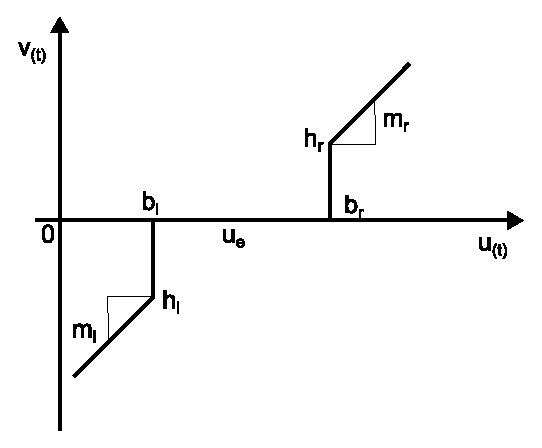
\includegraphics[width=0.45\textwidth]{images/chapter_1/zm_levitador.eps}
    \caption[Zona muerta centrada en el voltaje de equilibrio]{Zona muerta $v=D(u)$ centrada en el voltaje de equilibrio $u_e$, con pendientes $m_l$, $m_r$, umbrales $b_l$, $b_r$ y saltos $h_l$, $h_r$.}
    \label{fig:zm}
\end{figure}

La figura~\ref{fig:zm} muestra la forma de $D(u)$: mientras el voltaje comandado se mantenga dentro de la banda $(u_e+b_l,\,u_e+b_r)$, la salida $v$ del actuador es nula.

Como los parámetros de $D(u)$ no se conocen para el ECP-730, en las simulaciones se emplea una implementación simplificada con la misma asimetría de signos. Mientras el imán está en movimiento, el actuador no responde a cambios del voltaje comandado comprendidos entre $-0{,}02$ y $+0{,}025$~V respecto al último voltaje aplicado, que se mantiene; los cambios mayores se transmiten sin modificación. Cuando el imán está atascado, el voltaje comandado se aplica directamente. Esta implementación no es equivalente a $D(u)$. Tiene memoria, porque compara con el último voltaje aplicado en lugar de con $u_e$, y se desactiva mientras el imán está atascado. Los resultados de simulación valen, por tanto, para esta retención de voltaje y no para una zona muerta estática identificada del ECP-730. En una simulación adicional sin zona muerta, el ciclo límite del PII persiste con una amplitud un 8\,\% menor, de modo que la oscilación no necesita esta retención para aparecer. La identificación de los parámetros de $D(u)$ se propone como trabajo futuro.

La figura~\ref{lazo_de_control_con_zm} muestra el lazo de control completo, con la zona muerta entre el controlador y la planta.

\begin{figure}[ht]
    \centering
       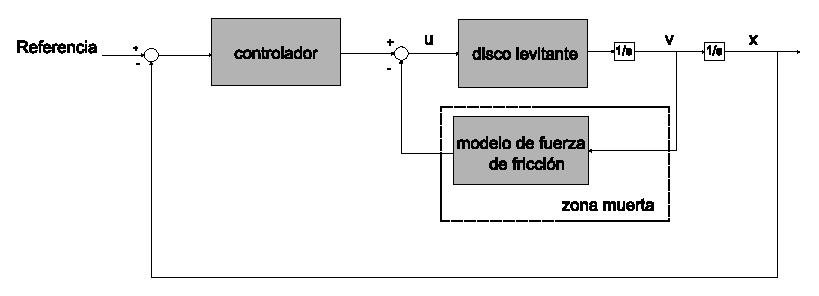
\includegraphics[width=0.6\textwidth]{images/chapter_1/lazo_de_control_con_zm.eps}
    \caption{Lazo de control con zona muerta}
    \label{lazo_de_control_con_zm}
\end{figure}

\section{Parámetros del modelo}\label{sec:parametros}

Los parámetros del modelo no lineal ($a$, $b$, $c_1$, $m$, $g$) fueron identificados experimentalmente por Hernández Alcántara~\cite{diana_tesis} para el dispositivo ECP-730 en configuración repulsiva (estable en lazo abierto), mediante ensayos de estado estacionario y respuesta dinámica en lazo abierto. En el presente trabajo se adoptan esos mismos parámetros y se aplican a la configuración atractiva (inestable en lazo abierto), en la que la bobina superior atrae al imán. La estructura funcional del modelo es idéntica en ambas configuraciones; en la atractiva, la fuerza magnética crece al disminuir la brecha entre el imán y la bobina, lo que hace que los puntos de equilibrio sean inestables.

La tabla~\ref{tab:parametros} reúne estos valores junto con los parámetros del modelo de fricción, el intervalo de la señal de control y la banda de la zona muerta simulada. Las fuerzas se expresan en $\text{kg}\cdot\text{cm}/\text{s}^2$, unidades en las que el peso del imán es $mg = 138{,}3$. En la tesis de Hernández Alcántara~\cite{diana_tesis}, $c_1$ se reporta en $\text{kg}^{-1}$; dado que multiplica a la velocidad en la ecuación de aceleración, sus unidades consistentes son $\text{s}^{-1}$. Por la misma razón, el valor de $b$ corresponde a fuerzas en $\text{kg}\cdot\text{cm}/\text{s}^2$, es decir, a voltios por $(\text{kg}\cdot\text{cm}/\text{s}^2)\cdot\text{cm}^4$. Ese antecedente lo reporta en $\text{V}/(\text{N}\cdot\text{cm}^4)$, y con esa unidad el valor equivalente sería $1{,}6163\times10^{-4}$, cien veces mayor. Con el valor y la unidad de la tabla~\ref{tab:parametros}, el modelo reproduce los voltajes de equilibrio que se usan en todo el trabajo.


\begin{table}[ht]
\centering
\caption{Parámetros del modelo}
\label{tab:parametros}
\begin{tabular}{|c|c|l|}
\hline
$a$ & $7{,}17184\;[\text{cm}]$ & parámetro de la fuerza electromagnética \\ \hline
$b$ & $1{,}6163 \times 10^{-6}\;[\text{V}\cdot\text{s}^2/(\text{kg}\cdot\text{cm}^5)]$ & parámetro de la fuerza electromagnética \\ \hline
$c_1$ & $8{,}563\;[\text{s}^{-1}]$ & fricción viscosa por unidad de masa \\ \hline
$m$ & $0{,}141\;[\text{kg}]$ & masa del imán \\ \hline
$g$ & $981\;[\text{cm}/\text{s}^2]$ & aceleración de la gravedad \\ \hline
$F_s$ & $20\;[\text{kg}\cdot\text{cm}/\text{s}^2]$ ($0{,}2$~N) & fricción estática máxima (Karnopp) \\ \hline
$DV$ & $0{,}02\;[\text{cm}/\text{s}]$ & banda de velocidad nula (Karnopp) \\ \hline
$u$ & $[0;\ 3{,}5]\;[\text{V}]$ & intervalo de la señal de control \\ \hline
$[b_l,\,b_r]$ & $[-0{,}02;\ +0{,}025]\;[\text{V}]$ & banda de la zona muerta simulada \\ \hline
\end{tabular}
\end{table}

\section{Modelo linealizado}\label{sec:linealizado}

Para diseñar el controlador se linealiza el modelo alrededor de una posición de equilibrio $x_1^{\ast}$, con el procedimiento general de la sección~\ref{sec:fund_linealizacion}. El modelo linealizado en espacio de estados para la configuración inestable es

\begin{equation}
\begin{aligned}
\dot{x}
&=
\begin{bmatrix}
0 & 1 \\[6pt]
\dfrac{4g}{(a-x_1^{\ast})} & -c_1
\end{bmatrix}x
+
\begin{bmatrix}
0 \\[6pt]
\dfrac{1}{mb\,(a-x_1^{\ast})^4}
\end{bmatrix}u,
\\[10pt]
y &= \begin{bmatrix} 1 & 0 \end{bmatrix} x .
\end{aligned}
\label{eq:lineal}
\end{equation}
En el modelo linealizado~\eqref{eq:lineal}, el vector de estado $x$ reúne la posición $x_1$ y la velocidad $x_2$ del imán, y la salida $y$ es la posición. El coeficiente $c_1$ de fricción viscosa por unidad de masa aparece en la matriz de estado como un amortiguamiento.

Su ecuación característica es
\begin{equation}
\lambda^2 + c_1\lambda - \dfrac{4g}{(a-x_1^{\ast})} = 0 .
\label{eq:caracteristica}
\end{equation}
Como $a - x_1^{\ast} > 0$ para toda posición alcanzable, el término independiente de la ecuación característica~\eqref{eq:caracteristica} es negativo y la ecuación tiene siempre una raíz real positiva: todos los puntos de equilibrio de la configuración atractiva son inestables. En $x_1^{\ast}=-4$~cm las raíces son $\lambda_1 = -23{,}5057$ y $\lambda_2 = 14{,}9427$.

Las matrices de controlabilidad y de observabilidad del modelo linealizado son
\begin{equation}
\mathcal{C}
=
\begin{bmatrix}
0 & \beta\\[6pt]
\beta & -c_1 \beta
\end{bmatrix} ,
\qquad
\mathcal{O}
=
\begin{bmatrix}
1 & 0\\[6pt]
0 & 1
\end{bmatrix} .
\label{eq:ctrb_obsv}
\end{equation}
La constante $\beta = 1/[m\,b\,(a-x_1^{\ast})^4]$ es la ganancia con la que el voltaje entra en la aceleración del imán. Las dos matrices~\eqref{eq:ctrb_obsv} tienen rango completo, de modo que el sistema es controlable y observable: con la entrada de la planta se puede llevar el estado a cualquier punto del espacio de estados, y a partir de la salida se puede determinar en qué punto se encuentra.

% Generado a partir de calculus/Final_Bien/evidencia_P8.m (simulador corregido).
\section{Comportamiento en lazo abierto}\label{sec:lazo_abierto}

Para caracterizar la inestabilidad de la configuración atractiva, se simuló el modelo no lineal sin fricción estática ni zona muerta, aplicando el voltaje de equilibrio $u=u_e(x_1^*)$ y desplazando la posición inicial $0{,}01$~cm respecto al equilibrio, en $x_1^*=-4$, $-3$ y $-2$~cm. La figura~\ref{fig:p8_lazo_abierto} muestra que la desviación crece exponencialmente y alcanza 1~cm en $0{,}33$, $0{,}32$ y $0{,}30$~s, respectivamente; el modelo linealizado reproduce el crecimiento con un tiempo de duplicación $\ln 2/\lambda_2$ de $46$, $44$ y $41$~ms. Cuanto más cerca de la bobina se encuentra el equilibrio, más rápido es el polo inestable.

\begin{figure}[ht]
    \centering
    % Estilo común de las figuras de evidencia P8 (pgfplots).
\pgfplotsset{
  pocho/.style={
    width=0.92\textwidth, height=5.2cm,
    grid=major, grid style={gray!25},
    tick label style={font=\small}, label style={font=\small}, legend style={font=\small},
    /pgf/number format/use comma,
    scaled ticks=false,
    y tick label style={/pgf/number format/fixed},
    table/col sep=comma, unbounded coords=jump,
    every axis plot/.append style={line join=round},
  },
}
\definecolor{tray}{RGB}{31,94,166}
\definecolor{refc}{RGB}{40,40,40}
\definecolor{ctl2}{RGB}{196,96,40}
\definecolor{ver}{RGB}{46,133,64}

\begin{tikzpicture}
\begin{semilogyaxis}[pocho, height=6cm, xmin=0, xmax=0.36, ymin=0.01, ymax=1,
    xlabel={tiempo [\si{s}]}, ylabel={$|x_1(t)-x_1^*|$ [\si{cm}]},
    x tick label style={/pgf/number format/fixed},
    legend style={at={(0.02,0.98)}, anchor=north west}, legend cell align=left]
  \addplot[tray, line width=1pt]  table[x=t, y=nl_m4] {images/p8_results/tikz/lazo_abierto.csv}; \addlegendentry{$x_1^*=-4$ cm}
  \addplot[ctl2, line width=1pt]  table[x=t, y=nl_m3] {images/p8_results/tikz/lazo_abierto.csv}; \addlegendentry{$x_1^*=-3$ cm}
  \addplot[ver, line width=1pt]   table[x=t, y=nl_m2] {images/p8_results/tikz/lazo_abierto.csv}; \addlegendentry{$x_1^*=-2$ cm}
  \addplot[tray, densely dashed]  table[x=t, y=lin_m4] {images/p8_results/tikz/lazo_abierto.csv}; \addlegendentry{modelo lineal}
  \addplot[ctl2, densely dashed, forget plot] table[x=t, y=lin_m3] {images/p8_results/tikz/lazo_abierto.csv};
  \addplot[ver, densely dashed, forget plot]  table[x=t, y=lin_m2] {images/p8_results/tikz/lazo_abierto.csv};
\end{semilogyaxis}
\end{tikzpicture}

    \caption[Lazo abierto en los puntos de equilibrio]{Desviación respecto al equilibrio en lazo abierto, con $u=u_e$ y una perturbación inicial de $0{,}01$~cm. Líneas continuas: modelo no lineal; discontinuas: modelo linealizado.}
    \label{fig:p8_lazo_abierto}
\end{figure}

El retrato de fase alrededor de $x_1^*=-4$~cm (figura~\ref{fig:p8_retrato}) confirma que el equilibrio es un punto silla: las trayectorias se alejan a lo largo de la variedad inestable, salvo las que parten exactamente sobre la variedad estable.


\begin{figure}[ht]
    \centering
    % Estilo común de las figuras de evidencia P8 (pgfplots).
\pgfplotsset{
  pocho/.style={
    width=0.92\textwidth, height=5.2cm,
    grid=major, grid style={gray!25},
    tick label style={font=\small}, label style={font=\small}, legend style={font=\small},
    /pgf/number format/use comma,
    scaled ticks=false,
    y tick label style={/pgf/number format/fixed},
    table/col sep=comma, unbounded coords=jump,
    every axis plot/.append style={line join=round},
  },
}
\definecolor{tray}{RGB}{31,94,166}
\definecolor{refc}{RGB}{40,40,40}
\definecolor{ctl2}{RGB}{196,96,40}
\definecolor{ver}{RGB}{46,133,64}

\begin{tikzpicture}
\begin{axis}[pocho, width=0.8\textwidth, height=7.5cm, xmin=-4.5, xmax=-3.5, ymin=-10, ymax=10,
    xlabel={posición $x_1$ [\si{cm}]}, ylabel={velocidad $x_2$ [\si{cm/s}]},
    legend style={at={(0.98,0.02)}, anchor=south east, fill=white}, legend cell align=left]
  \addplot[gray!60, quiver={u=\thisrow{dx}, v=\thisrow{dv}, every arrow/.append style={-stealth}}, forget plot]
    table[x=x, y=v] {images/p8_results/tikz/campo.csv};
  \addplot[tray, line width=0.9pt] table[x=x, y=v] {images/p8_results/tikz/trayectorias.csv}; \addlegendentry{trayectorias}
  \addplot[ctl2, line width=1.4pt] table[x=x, y=v] {images/p8_results/tikz/variedad_inestable.csv}; \addlegendentry{variedad inestable}
  \addplot[ver, line width=3pt, opacity=0.6] coordinates {(-4.4448,0) (-3.6291,0)}; \addlegendentry{banda de atascamiento ($u=u_e$)}
  \addplot[only marks, mark=*, mark size=2pt, refc] coordinates {(-4,0)}; \addlegendentry{equilibrio $x_1^*=-4$ cm}
\end{axis}
\end{tikzpicture}

    \caption[Retrato de fase en lazo abierto]{Retrato de fase del modelo no lineal sin fricción estática alrededor de $x_1^*=-4$~cm, con $u=u_e$. La banda verde indica las posiciones en las que, con el imán en reposo, la fricción estática lo mantiene atascado.}
    \label{fig:p8_retrato}
\end{figure}

Al incorporar la fricción estática de Karnopp cambia la situación en reposo: si el imán está detenido y $u=u_e$, la fuerza neta $u/[b(a-x)^4]-mg$ no supera $F_s$ mientras la posición se encuentre entre $-4{,}44$ y $-3{,}63$~cm, de modo que el imán permanece atascado en cualquier punto de esa banda. Para $x_1^*=-3$ y $-2$~cm las bandas correspondientes son $[-3{,}41;\,-2{,}66]$ y $[-2{,}37;\,-1{,}70]$~cm. La fricción estática enmascara así la inestabilidad del equilibrio mientras el imán no se mueva.

\FloatBarrier

\section{Análisis estático del actuador}\label{sec:actuador_estatico}

El voltaje que puede aplicar el actuador está acotado a $u\in[0;\,3{,}5]$~V, y esa cota determina en qué posiciones puede operar el sistema. Para sostener el imán en $x_1$ se necesita el voltaje de equilibrio~\eqref{eq:ue}, que crece rápidamente al alejarse de la bobina: $1{,}58$~V en $-2$~cm, $2{,}39$~V en $-3$~cm, $3{,}48$~V en $-4$~cm y $4{,}91$~V en $-5$~cm. Para mover el imán hay que vencer además la fricción estática, lo que exige llegar a $u_e(1\pm F_s/mg)$, es decir, a un $14{,}5$\,\% por encima o por debajo del equilibrio. La sección~\ref{sec:analisis_ciclo} retoma esta banda para explicar el ciclo límite.

En $x_1=-4$~cm, el punto en que se linealizó el modelo para el diseño, el imán puede sostenerse con $3{,}48$~V, pero no subir: para despegarlo hacia la bobina se requieren unos $3{,}99$~V, por encima de la cota de $3{,}5$~V. Sí puede despegarse hacia abajo si el voltaje baja de unos $2{,}98$~V, pero entonces se aleja de la bobina, el voltaje de equilibrio crece todavía más y el actuador ya no puede recuperarlo. Desde $-4$~cm el imán no tiene, por tanto, ningún movimiento regulable, aunque sí puede caer. El barrido de escalones del capítulo~\ref{chap:desempeno} determina qué posiciones y qué cambios de referencia son alcanzables con $u\le3{,}5$~V, y de él se obtiene el intervalo de pruebas.

El modelo queda así completo: una planta inestable en lazo abierto, con fricción estática que puede mantener al imán detenido y un actuador acotado, con zona muerta, que limita dónde se puede actuar. Sobre el modelo linealizado se diseña, en el capítulo siguiente, el controlador.

 \chapter{Diseño del controlador}\label{chap:controlador}

El capítulo~\ref{chap:modelo} dejó establecida la planta y sus límites. Este capítulo responde a la pregunta siguiente: qué controlador lineal estabiliza esa planta y con qué holgura. Se toma la planta linealizada en el punto de diseño y se fijan los objetivos, se presenta el PII, se examina su robustez en el intervalo de operación y, por último, se define el controlador de comparación con una sola acción integral. Cuánto logra el PII frente a las no linealidades no suaves se evalúa en los capítulos~\ref{chap:desempeno} y~\ref{chap:doble_integral}.

\section{Planta linealizada y objetivos del diseño}\label{sec:planta_diseno}

El diseño parte del modelo linealizado~\eqref{eq:lineal} del capítulo~\ref{chap:modelo}, evaluado en el punto de equilibrio $x_1^*=-4$~cm. La entrada es el voltaje del actuador y la salida es la posición del imán. Con esos datos, la función de transferencia de la planta es
\begin{equation}
G(s)=\frac{281{,}7}{s^{2}+8{,}563\,s-351{,}2} .
\label{eq:planta}
\end{equation}
El numerador $281{,}7$ es la ganancia de entrada $1/\bigl(mb(a-x_1^*)^4\bigr)$ del modelo~\eqref{eq:lineal}, y el término independiente del denominador, $-351{,}2$, es el valor de $4g/(a-x_1^*)$ de la ecuación característica~\eqref{eq:caracteristica}. Su signo negativo produce un polo real en el semiplano derecho, en $14{,}94$~rad/s, que es la inestabilidad en lazo abierto de la configuración atractiva descrita en el capítulo~\ref{chap:introduccion}. El coeficiente $8{,}563$ es la fricción viscosa $c_1$.

El controlador debe cumplir cuatro objetivos. Debe estabilizar el lazo, para lo cual el diagrama de Nyquist ha de rodear el punto $-1$ una vez en sentido antihorario, como exige el criterio con un polo inestable (sección~\ref{sec:fund_nyquist}). Debe dejar márgenes de estabilidad razonables. Debe anular el error estacionario ante escalones y rampas, lo que pide un lazo de tipo dos (sección~\ref{sec:fund_tipo}). Y debe proporcionar alta ganancia a baja frecuencia, la motivación de la doble acción integral expuesta en la sección~\ref{sec:motivacion} del capítulo~\ref{chap:introduccion}.

\section{El controlador con doble acción integral}\label{sec:pii}

El controlador se ajustó sobre la planta~\eqref{eq:planta}, de forma interactiva en los editores de Bode y del lugar de las raíces del \emph{Control System Designer} de MATLAB. El resultado es
\begin{equation}
C(s)=\frac{152{,}43\,(s+4{,}875)(s+1{,}861)(s+17{,}31)}
{s^{2}(s+301{,}1)} .
\label{eq:pii}
\end{equation}

\subsection{Estructura}

El controlador~\eqref{eq:pii} tiene tres partes. El doble integrador $1/s^2$ hace al lazo de tipo dos, lo que anula el error estacionario ante escalones y rampas, y proporciona la acción acumulada que se espera que ayude a salir de la zona muerta. Los ceros en $-1{,}861$ y $-4{,}875$~rad/s compensan el atraso de fase de los dos integradores por debajo de la frecuencia de cruce. El par cero-polo en $-17{,}31$ y $-301{,}1$~rad/s actúa como red de adelanto, con su máximo aporte de fase cerca de $72$~rad/s.

\subsection{Márgenes de estabilidad}

Con esta estructura, el lazo abierto $L(s)=C(s)G(s)$ tiene un margen de fase de $59{,}9^\circ$ en $129{,}3$~rad/s (figura~\ref{bode_fase}). Como la planta tiene un polo inestable, el margen de ganancia es inferior (sección~\ref{sec:fund_nyquist}): el lazo sigue siendo estable si la ganancia aumenta, pero se inestabiliza si disminuye por debajo de $0{,}14$ veces su valor nominal ($-17{,}1$~dB en $9{,}63$~rad/s). Los polos del lazo cerrado son $-143{,}3\pm133{,}7\mathrm{j}$, $-14{,}10$, $-7{,}28$ y $-1{,}71$, todos en el semiplano izquierdo.

\begin{figure}[ht]
    \centering
    % Estilo común de las figuras de diseño del PII (pgfplots).
\input{images/pii_design/tikz/valores}
\pgfplotsset{
  diseno/.style={
    grid=major, grid style={gray!25},
    tick label style={font=\small}, label style={font=\small}, legend style={font=\small},
    /pgf/number format/use comma,
    table/col sep=comma,
    every axis plot/.append style={line join=round},
  },
}
\definecolor{tray}{RGB}{31,94,166}
\definecolor{marg}{RGB}{196,96,40}
\definecolor{refc}{RGB}{40,40,40}

\begin{tikzpicture}
\begin{axis}[diseno, name=mag, width=0.85\textwidth, height=5.2cm, xmode=log,
             xmin=1e-2, xmax=1e4, ymin=-100, ymax=110, ytick={-100,-50,0,50,100},
             xticklabels={}, ylabel={magnitud [\si{dB}]}]
  \addplot[refc!50, densely dashed] coordinates {(1e-2,0) (1e4,0)};
  \addplot[tray, line width=1pt] table[x=w, y=mag_db] {images/pii_design/tikz/bode.csv};
  \draw[marg, line width=0.8pt] (axis cs:\PIIwg,0) -- (axis cs:\PIIwg,\PIImgwg);
  \addplot[marg, only marks, mark=*, mark size=1.8pt] coordinates {(\PIIwg,\PIImgwg)};
  \node[font=\small, anchor=north east, align=left, fill=white, inner sep=2pt]
    at (axis cs:8e3,104) {MG $=\num{\PIIgmdb}$~\si{dB} en $\omega=\num[round-mode=places,round-precision=2]{\PIIwg}$~\si{rad/s}};
\end{axis}
\begin{axis}[diseno, at={(mag.south west)}, anchor=north west, yshift=-0.35cm,
             width=0.85\textwidth, height=5.2cm, xmode=log,
             xmin=1e-2, xmax=1e4, ymin=-375, ymax=-90, ytick={-360,-315,-270,-225,-180,-135},
             xlabel={frecuencia [\si{rad/s}]}, ylabel={fase [\si{\degree}]}]
  \addplot[refc!50, densely dashed] coordinates {(1e-2,-180) (1e4,-180)};
  \addplot[tray, line width=1pt] table[x=w, y=fase] {images/pii_design/tikz/bode.csv};
  \draw[marg, line width=0.8pt] (axis cs:\PIIwp,-180) -- (axis cs:\PIIwp,\PIIphwp);
  \addplot[marg, only marks, mark=*, mark size=1.8pt] coordinates {(\PIIwp,\PIIphwp)};
  \node[font=\small, anchor=south east, align=left, fill=white, inner sep=2pt]
    at (axis cs:8e3,-370) {MF $=\num{\PIIpm}\si{\degree}$ en $\omega=\num[round-mode=places,round-precision=1]{\PIIwp}$~\si{rad/s}};
\end{axis}
\end{tikzpicture}

    \caption[Diagrama de Bode]{Diagrama de Bode del lazo abierto $L(s)=C(s)G(s)$ en $x_1^*=-4$~cm. Se indican el margen de ganancia (inferior, por el polo inestable de la planta) y el margen de fase.}
    \label{bode_fase}
\end{figure}

El diagrama de Nyquist (figura~\ref{nyquist}) rodea una vez el punto $-1$ en sentido antihorario, que es el rodeo que exige el criterio con un polo inestable en lazo abierto.

\begin{figure}[ht]
    \centering
    % Estilo común de las figuras de diseño del PII (pgfplots).
\input{images/pii_design/tikz/valores}
\pgfplotsset{
  diseno/.style={
    grid=major, grid style={gray!25},
    tick label style={font=\small}, label style={font=\small}, legend style={font=\small},
    /pgf/number format/use comma,
    table/col sep=comma,
    every axis plot/.append style={line join=round},
  },
}
\definecolor{tray}{RGB}{31,94,166}
\definecolor{marg}{RGB}{196,96,40}
\definecolor{refc}{RGB}{40,40,40}

\begin{tikzpicture}
\begin{axis}[diseno, width=0.8\textwidth, height=0.62\textwidth,
             xmin=-10, xmax=2, ymin=-7, ymax=7, axis equal image,
             xlabel={$\operatorname{Re}\{L(j\omega)\}$}, ylabel={$\operatorname{Im}\{L(j\omega)\}$},
             legend pos=north west, legend cell align=left]
  \addplot[refc!40, thin, forget plot] coordinates {(-10,0) (2,0)};
  \addplot[refc!40, thin, forget plot] coordinates {(0,-7) (0,7)};
  \addplot[refc!55, densely dashed, domain=0:360, samples=120, forget plot] ({cos(x)},{sin(x)});
  \addplot[tray, line width=1pt]
    table[x=re, y=im] {images/pii_design/tikz/nyquist_pos.csv};
  \addlegendentry{$\omega>0$}
  \addplot[tray!55, line width=0.8pt, densely dashed]
    table[x=re, y=im] {images/pii_design/tikz/nyquist_neg.csv};
  \addlegendentry{$\omega<0$}
  \addplot[red!75!black, only marks, mark=+, mark size=4pt, line width=1.2pt] coordinates {(-1,0)};
  \addlegendentry{$-1$}
  \draw[tray, -stealth, line width=1pt] \PIIflechaA;
  \draw[tray, -stealth, line width=1pt] \PIIflechaB;
  \draw[tray!55, -stealth, line width=0.8pt] \PIIflechaC;
  \draw[tray!55, -stealth, line width=0.8pt] \PIIflechaD;
  \draw[marg, thin] (axis cs:-7.14,0) -- (axis cs:-8.5,-1.2);
  \node[font=\small, anchor=north, fill=white, inner sep=1.5pt] at (axis cs:-8.5,-1.2) {$-1/\mathrm{MG}$};
  \addplot[marg, only marks, mark=*, mark size=1.6pt, forget plot] coordinates {(-7.14,0)};
\end{axis}
\end{tikzpicture}

    \caption[Diagrama de Nyquist]{Diagrama de Nyquist de $L(s)$. Con un polo de lazo abierto en el semiplano derecho ($P=1$), la estabilidad en lazo cerrado exige un rodeo antihorario al punto $-1$.}
    \label{nyquist}
\end{figure}

\subsection{Respuesta al escalón}

En lazo cerrado lineal, la respuesta al escalón (figura~\ref{step_response}) tiene un tiempo de subida de $9{,}3$~ms, un sobrepaso de $16{,}9$\,\% con pico de $1{,}169$ en $23{,}8$~ms y un tiempo de establecimiento de $0{,}284$~s.

\begin{figure}[ht]
    \centering
    % Estilo común de las figuras de diseño del PII (pgfplots).
\input{images/pii_design/tikz/valores}
\pgfplotsset{
  diseno/.style={
    grid=major, grid style={gray!25},
    tick label style={font=\small}, label style={font=\small}, legend style={font=\small},
    /pgf/number format/use comma,
    table/col sep=comma,
    every axis plot/.append style={line join=round},
  },
}
\definecolor{tray}{RGB}{31,94,166}
\definecolor{marg}{RGB}{196,96,40}
\definecolor{refc}{RGB}{40,40,40}

\begin{tikzpicture}
\begin{axis}[diseno, width=0.85\textwidth, height=6cm, xmin=0, xmax=0.6, ymin=0, ymax=1.32,
             xlabel={tiempo [\si{s}]}, ylabel={amplitud},
             xtick={0,0.1,...,0.6}, x tick label style={/pgf/number format/fixed}]
  \addplot[refc!55, densely dashed] coordinates {(0,1) (0.6,1)};
  \addplot[refc!30, densely dotted, forget plot] coordinates {(0,0.98) (0.6,0.98)};
  \addplot[refc!30, densely dotted, forget plot] coordinates {(0,1.02) (0.6,1.02)};
  \addplot[tray, line width=1pt] table[x=t, y=y] {images/pii_design/tikz/escalon.csv};
  \addplot[marg, only marks, mark=*, mark size=1.8pt] coordinates {(\PIItp,\PIIyp)};
  \node[font=\small, anchor=south west, inner sep=2pt] at (axis cs:\PIItp,\PIIyp)
    {sobrepaso \SI{\PIIos}{\percent}};
  \draw[marg, densely dashed] (axis cs:\PIIts,0) -- (axis cs:\PIIts,0.98);
  \node[font=\small, anchor=south west, fill=white, inner sep=2pt] at (axis cs:\PIIts,0.08)
    {$t_s=\num{\PIIts}$~\si{s} (\SI{2}{\percent})};
\end{axis}
\end{tikzpicture}

    \caption[Respuesta al escalón]{Respuesta al escalón unitario del lazo cerrado linealizado.}
    \label{step_response}
\end{figure}

\section{Robustez en el intervalo de operación}\label{sec:robustez_pii}

El controlador se diseñó en $-4$~cm, pero las pruebas se hacen entre $-3$ y $-2$~cm. La sección~\ref{sec:actuador_estatico} del capítulo~\ref{chap:modelo} justifica ese intervalo por el voltaje que el actuador puede entregar, y la sección~\ref{sec:intervalo} del capítulo~\ref{chap:desempeno} lo confirma con un barrido de escalones. Conviene entonces saber si el diseño se sostiene donde se opera. Al acercarse el imán a la bobina, el polo inestable se desplaza hacia la derecha, de $14{,}94$ a $16{,}84$~rad/s, y la planta se vuelve más difícil de estabilizar. La tabla~\ref{tab:pii_intervalo} reúne el margen de fase y el sobrepaso lineal del mismo controlador~\eqref{eq:pii}, sin reajuste, sobre la planta linealizada en cada posición.

\begin{table}[ht]
    \centering
    \caption[PII en el intervalo de operación]{Controlador PII~\eqref{eq:pii}, diseñado en $-4$~cm, evaluado sobre la planta linealizada en las posiciones de prueba.}
    \label{tab:pii_intervalo}
    \begin{tabular}{rccc}
        \hline
        $x_1^*$ [cm] & Polo inestable [rad/s] & Margen de fase & Sobrepaso lineal \\
        \hline
        $-4{,}0$ (diseño) & $14{,}94$ & $59{,}9^\circ$ & $16{,}9$\,\% \\
        $-3{,}0$ & $15{,}82$ & $54{,}5^\circ$ & $19{,}2$\,\% \\
        $-2{,}5$ & $16{,}31$ & $51{,}1^\circ$ & $21{,}6$\,\% \\
        $-2{,}0$ & $16{,}84$ & $47{,}4^\circ$ & $24{,}7$\,\% \\
        \hline
    \end{tabular}
\end{table}

El lazo permanece estable en todo el intervalo, con menos margen conforme el imán se acerca a la bobina. El margen de fase baja de $59{,}9^\circ$ a $47{,}4^\circ$ y el sobrepaso lineal sube de $16{,}9$\,\% a $24{,}7$\,\%. El controlador, por tanto, no necesita reajustarse para operar entre $-3$ y $-2$~cm, y todas las pruebas de los capítulos siguientes lo emplean tal como está.

\section{El controlador PI de comparación}\label{sec:pi}

La pregunta central del trabajo es qué aporta la segunda integración. Para responderla se necesita un controlador de referencia que difiera del PII en eso y en poco más. El controlador PI de comparación es
\begin{equation}
C_{PI}(s)=\frac{178{,}14\,(s+15)(s+12{,}91)}{s\,(s+400)} .
\label{eq:pi}
\end{equation}
A diferencia del PII~\eqref{eq:pii}, tiene un solo integrador, de modo que el lazo es de tipo uno y su ganancia a baja frecuencia crece más lentamente. Conserva la red de adelanto, con un polo en $-400$~rad/s, y dos ceros en $-15$ y $-12{,}91$~rad/s. Sobre la planta~\eqref{eq:planta} tiene un margen de fase de $64{,}1^\circ$ en $118{,}6$~rad/s, un sobrepaso lineal de $17{,}6$\,\% y un tiempo de establecimiento lineal de $0{,}240$~s. Estos valores son comparables a los del PII ($59{,}9^\circ$, $16{,}9$\,\% y $0{,}284$~s), de modo que la diferencia entre ambos lazos queda en la segunda acción integral y no en una respuesta lineal mejor o peor sintonizada.

Este controlador servirá en el capítulo~\ref{chap:doble_integral} para aislar el efecto de la segunda integración sobre el comportamiento con atascamiento-deslizamiento y zona muerta. Antes, el capítulo~\ref{chap:desempeno} evalúa el desempeño del PII en simulación.

 \chapter{Desempeño en simulación}\label{chap:desempeno}

El capítulo~\ref{chap:controlador} diseñó el controlador PII sobre el modelo linealizado en $-4$~cm. Este capítulo responde a la pregunta que sigue: qué hace ese controlador cuando se conecta a la planta completa, con su fuerza electromagnética no lineal, su zona muerta y su fricción estática. Se delimita primero el intervalo en que el actuador permite operar; después se prueba el lazo en regulación, primero sin y luego con atascamiento-deslizamiento, y se aísla mediante el modelo lineal la causa de lo que aparece. Se evalúa a continuación el seguimiento de referencias senoidales y trapezoidales y, por último, el comportamiento en la configuración estable. En todo el capítulo se \emph{describe} lo que se observa; el capítulo~\ref{chap:doble_integral} explica por qué ocurre.

\section{Intervalo de operación}
\label{sec:intervalo}

El actuador está acotado a $u\in[0;\,3{,}5]$~V, y la sección~\ref{sec:actuador_estatico} del capítulo~\ref{chap:modelo} muestra que con esa cota el imán puede sostenerse en $-4$~cm, el punto de diseño, pero no subir desde ahí. Para delimitar en qué posiciones sí puede desplazarse de forma regulada, se simularon 7503 escalones con distintas posiciones iniciales y finales, con el PII y con el PI, en presencia de atascamiento-deslizamiento. Una referencia se considera alcanzable si el imán se sostiene en la posición inicial antes del escalón, no diverge, y en los últimos 5~s de la simulación de 40~s el error se mantiene por debajo de $0{,}05$~cm. La tabla~\ref{tab:intervalo} resume el resultado con el PII.

\begin{table}[ht]
\centering
\caption{Referencias alcanzables con $u\le3{,}5$~V desde distintas posiciones iniciales (PII, con atascamiento-deslizamiento).}
\label{tab:intervalo}
\begin{tabular}{|c|c|}
\hline
Posición inicial [cm] & Referencias alcanzables [cm] \\ \hline
$-4{,}0$ & ninguna: el imán se sostiene pero no sube \\ \hline
$-3{,}5$ & de $-3{,}6$ a $-2{,}0$ \\ \hline
$-3{,}0$ & de $-3{,}5$ a $-1{,}5$ \\ \hline
$-2{,}0$ & de $-3{,}3$ a $-0{,}5$ \\ \hline
$-1{,}0$ & de $-2{,}5$ a $+0{,}5$ \\ \hline
\end{tabular}
\end{table}

Desde $-4$~cm, el criterio marca también como alcanzable la referencia de $-3{,}95$~cm, pero solo porque está a menos de $0{,}05$~cm de la posición inicial, sin que el imán se mueva; la tabla no la cuenta. Los cambios de referencia son viables a partir de unos $-3{,}6$~cm. Por ello, las pruebas de este capítulo se realizan en el intervalo de $-3$ a $-2$~cm, con un escalón de $-2$ a $-3$~cm que deja margen respecto a ambos límites. Los márgenes de estabilidad del PII en ese intervalo se presentaron en la sección~\ref{sec:robustez_pii}.

\section{Simulación no lineal sin atascamiento-deslizamiento}

La primera prueba establece la referencia ideal. El controlador PII se evaluó sobre el modelo no lineal del levitador con la fuerza electromagnética no lineal y la fricción viscosa únicamente,
\begin{equation}
m\ddot{x} = \frac{u}{b\,(a-x)^4} - m g - m c_1 \dot{x} ,
\label{eq:nl_sin_ad}
\end{equation}
es decir, sin la fricción estática de Karnopp ni la zona muerta del actuador que las secciones~\ref{sec:friccion_modelo} y~\ref{sec:zm_modelo} incorporan a la ecuación de movimiento~\eqref{eq:mec}. Las condiciones son las de la prueba de regulación de la sección~\ref{sec:regulacion}: escalón de referencia de $-2$ a $-3$~cm en $t=10$~s, señal de control acotada a $u\in[0;\,3{,}5]$~V y controlador inicializado en el estado estacionario correspondiente a $x_1=-2$~cm. Para facilitar la comparación, cada figura superpone el resultado con atascamiento-deslizamiento (AD), que se presenta en esa misma sección.

\begin{figure}[ht]
    \centering
    % Estilo común de las figuras sin/con atascamiento-deslizamiento (pgfplots).
\pgfplotsset{
  sinad/.style={
    width=0.92\textwidth, height=5.2cm, xmin=0, xmax=40,
    xlabel={tiempo [\si{s}]},
    grid=major, grid style={gray!25},
    tick label style={font=\small}, label style={font=\small}, legend style={font=\small},
    /pgf/number format/use comma,
    scaled ticks=false,
    y tick label style={/pgf/number format/fixed},
    table/col sep=comma,
    every axis plot/.append style={line join=round},
  },
  detalle/.style={height=4cm, axis background/.style={fill=ctl2!4}},
  sinAD/.style={tray, line width=1.1pt},
  conAD/.style={ctl2, line width=0.7pt},
}
\definecolor{tray}{RGB}{31,94,166}
\definecolor{refc}{RGB}{40,40,40}
\definecolor{ctl2}{RGB}{196,96,40}

\begin{tikzpicture}
\begin{axis}[sinad, name=principal, xlabel={}, ylabel={posición [\si{cm}]}, ymin=-3.35, ymax=-1.85,
             legend style={at={(0.99,0.97)}, anchor=north east}, legend cell align=left]
  \addplot[conAD] table[x=t, y=x_ad] {images/sin_ad_results/tikz/comparacion.csv};
  \addlegendentry{con AD}
  \addplot[sinAD] table[x=t, y=x] {images/sin_ad_results/tikz/comparacion.csv};
  \addlegendentry{sin AD}
  \addplot[refc, densely dashed, line width=0.8pt] table[x=t, y=r] {images/sin_ad_results/tikz/comparacion.csv};
  \addlegendentry{referencia}
  \fill[ctl2, opacity=0.15] (axis cs:9.8,-3.35) rectangle (axis cs:12,-1.85);
\end{axis}
\begin{axis}[sinad, detalle, at={(principal.south west)}, anchor=north west, yshift=-0.45cm,
             xmin=9.8, xmax=12, ymin=-3.3, ymax=-1.9, ylabel={detalle [\si{cm}]}]
  \addplot[conAD, line width=1.6pt] table[x=t, y=x_ad] {images/sin_ad_results/tikz/detalle.csv};
  \addplot[sinAD, line width=0.8pt] table[x=t, y=x] {images/sin_ad_results/tikz/detalle.csv};
  \addplot[refc, densely dashed, line width=0.8pt] table[x=t, y=r] {images/sin_ad_results/tikz/detalle.csv};
\end{axis}
\end{tikzpicture}

    \caption[Sin AD: posición]{Posición del imán con el modelo no lineal sin atascamiento-deslizamiento (sin AD) y con él (con AD). Abajo, detalle del transitorio entre 9,8 y 12~s.}
    \label{fig:sinad_pos}
\end{figure}

\begin{figure}[ht]
    \centering
    % Estilo común de las figuras sin/con atascamiento-deslizamiento (pgfplots).
\pgfplotsset{
  sinad/.style={
    width=0.92\textwidth, height=5.2cm, xmin=0, xmax=40,
    xlabel={tiempo [\si{s}]},
    grid=major, grid style={gray!25},
    tick label style={font=\small}, label style={font=\small}, legend style={font=\small},
    /pgf/number format/use comma,
    scaled ticks=false,
    y tick label style={/pgf/number format/fixed},
    table/col sep=comma,
    every axis plot/.append style={line join=round},
  },
  detalle/.style={height=4cm, axis background/.style={fill=ctl2!4}},
  sinAD/.style={tray, line width=1.1pt},
  conAD/.style={ctl2, line width=0.7pt},
}
\definecolor{tray}{RGB}{31,94,166}
\definecolor{refc}{RGB}{40,40,40}
\definecolor{ctl2}{RGB}{196,96,40}

\begin{tikzpicture}
\begin{axis}[sinad, ylabel={velocidad [\si{cm/s}]},
             legend style={at={(0.99,0.03)}, anchor=south east}, legend cell align=left]
  \addplot[conAD] table[x=t, y=v_ad] {images/sin_ad_results/tikz/comparacion.csv};
  \addlegendentry{con AD}
  \addplot[sinAD] table[x=t, y=v] {images/sin_ad_results/tikz/comparacion.csv};
  \addlegendentry{sin AD}
\end{axis}
\end{tikzpicture}

    \caption[Sin AD: velocidad]{Velocidad del imán sin y con atascamiento-deslizamiento.}
    \label{fig:sinad_vel}
\end{figure}

\begin{figure}[ht]
    \centering
    % Estilo común de las figuras sin/con atascamiento-deslizamiento (pgfplots).
\pgfplotsset{
  sinad/.style={
    width=0.92\textwidth, height=5.2cm, xmin=0, xmax=40,
    xlabel={tiempo [\si{s}]},
    grid=major, grid style={gray!25},
    tick label style={font=\small}, label style={font=\small}, legend style={font=\small},
    /pgf/number format/use comma,
    scaled ticks=false,
    y tick label style={/pgf/number format/fixed},
    table/col sep=comma,
    every axis plot/.append style={line join=round},
  },
  detalle/.style={height=4cm, axis background/.style={fill=ctl2!4}},
  sinAD/.style={tray, line width=1.1pt},
  conAD/.style={ctl2, line width=0.7pt},
}
\definecolor{tray}{RGB}{31,94,166}
\definecolor{refc}{RGB}{40,40,40}
\definecolor{ctl2}{RGB}{196,96,40}

\begin{tikzpicture}
\begin{axis}[sinad, name=principal, xlabel={}, ylabel={error [\si{cm}]},
             legend style={at={(0.99,0.03)}, anchor=south east}, legend cell align=left]
  \addplot[conAD] table[x=t, y=e_ad] {images/sin_ad_results/tikz/comparacion.csv};
  \addlegendentry{con AD}
  \addplot[sinAD] table[x=t, y=e] {images/sin_ad_results/tikz/comparacion.csv};
  \addlegendentry{sin AD}
  \fill[ctl2, opacity=0.15] ({axis cs:15,0} |- {rel axis cs:0,0}) rectangle ({axis cs:40,0} |- {rel axis cs:0,1});
\end{axis}
\begin{axis}[sinad, detalle, at={(principal.south west)}, anchor=north west, yshift=-0.45cm,
             xmin=15, xmax=40, ymin=-0.03, ymax=0.03, ylabel={detalle [\si{cm}]}]
  \addplot[refc!60, thin] coordinates {(15,0) (40,0)};
  \addplot[conAD] table[x=t, y=e_ad] {images/sin_ad_results/tikz/comparacion.csv};
  \addplot[sinAD] table[x=t, y=e] {images/sin_ad_results/tikz/comparacion.csv};
\end{axis}
\end{tikzpicture}

    \caption[Sin AD: error]{Error de posición sin y con atascamiento-deslizamiento. Abajo, detalle entre 15 y 40~s.}
    \label{fig:sinad_error}
\end{figure}

\begin{figure}[ht]
    \centering
    % Estilo común de las figuras sin/con atascamiento-deslizamiento (pgfplots).
\pgfplotsset{
  sinad/.style={
    width=0.92\textwidth, height=5.2cm, xmin=0, xmax=40,
    xlabel={tiempo [\si{s}]},
    grid=major, grid style={gray!25},
    tick label style={font=\small}, label style={font=\small}, legend style={font=\small},
    /pgf/number format/use comma,
    scaled ticks=false,
    y tick label style={/pgf/number format/fixed},
    table/col sep=comma,
    every axis plot/.append style={line join=round},
  },
  detalle/.style={height=4cm, axis background/.style={fill=ctl2!4}},
  sinAD/.style={tray, line width=1.1pt},
  conAD/.style={ctl2, line width=0.7pt},
}
\definecolor{tray}{RGB}{31,94,166}
\definecolor{refc}{RGB}{40,40,40}
\definecolor{ctl2}{RGB}{196,96,40}

\begin{tikzpicture}
\begin{axis}[sinad, ylabel={señal de control [\si{V}]}, ymin=-0.2, ymax=3.8,
             legend style={at={(0.99,0.03)}, anchor=south east}, legend cell align=left, legend columns=3]
  \addplot[conAD] table[x=t, y=u_ad] {images/sin_ad_results/tikz/comparacion.csv};
  \addlegendentry{con AD}
  \addplot[sinAD] table[x=t, y=u] {images/sin_ad_results/tikz/comparacion.csv};
  \addlegendentry{sin AD}
  \addplot[red!70!black, densely dotted, line width=0.8pt] coordinates {(0,3.5) (40,3.5)};
  \addlegendentry{$u_{\max}$}
\end{axis}
\end{tikzpicture}

    \caption[Sin AD: señal de control]{Señal de control sin y con atascamiento-deslizamiento.}
    \label{fig:sinad_ctrl}
\end{figure}

La figura~\ref{fig:sinad_pos} muestra que, sin AD, el lazo cerrado no lineal alcanza la nueva referencia con un sobrepaso de $23{,}7$\,\% a los $0{,}15$~s del escalón y entra en la banda de $\pm 2$\,\% del cambio de referencia en $0{,}48$~s. Este sobrepaso se encuentra entre los que predice el modelo linealizado en $x_1^*=-3$~cm ($19{,}2$\,\%) y en $x_1^*=-2$~cm ($24{,}7$\,\%), lo que confirma la coherencia entre el modelo empleado para el diseño y la planta no lineal. La velocidad (figura~\ref{fig:sinad_vel}) se anula una vez concluido el transitorio, el error (figura~\ref{fig:sinad_error}) converge a cero y la señal de control (figura~\ref{fig:sinad_ctrl}) converge al voltaje de equilibrio $u_e=2{,}3934$~V correspondiente a $x_1=-3$~cm, sin alcanzar la saturación superior.

La comparación con el caso con AD muestra que el transitorio es prácticamente idéntico (sobrepaso de $23{,}6$\,\%). La diferencia aparece en estado estacionario, donde la fricción estática y la zona muerta sustituyen la convergencia asintótica por un ciclo límite de $0{,}033$~cm pico a pico. Con ello se cumple el tercer objetivo específico de la tesis (capítulo~\ref{chap:introduccion}): simular el desempeño del controlador en el modelo no lineal sin atascamiento-deslizamiento.

\FloatBarrier

\section{Regulación con atascamiento-deslizamiento}
\label{sec:regulacion}

La prueba de regulación aplica el mismo escalón de $-2$ a $-3$~cm en $t=10$~s al lazo completo: PII, zona muerta y fricción de Karnopp, con la señal de control acotada a $u\in[0;\,3{,}5]$~V. Se simulan 40~s con un periodo de muestreo de 1~ms; el controlador parte del estado estacionario correspondiente a $x_1=-2$~cm, de modo que antes del escalón el imán permanece en reposo.

La figura~\ref{posicion} muestra la respuesta. El imán alcanza un mínimo de $-3{,}236$~cm a los $0{,}15$~s del escalón, lo que equivale a un sobrepaso de $23{,}6$\,\%, y entra en la banda de $\pm0{,}05$~cm alrededor de la referencia a los $0{,}40$~s. A partir de ahí no se detiene sobre la referencia: oscila en un ciclo límite (\emph{hunting}, sección~\ref{sec:fund_friccion}) de $0{,}033$~cm pico a pico. En esta tesis, «ciclo límite» designa esa oscilación persistente observada en simulaciones de duración finita; no se demuestra que sea una órbita periódica aislada ni que atraiga a todas las trayectorias. La oscilación tiene un error máximo de $0{,}018$~cm y un error medio de $6\times10^{-5}$~cm en los últimos 10~s. La velocidad (figura~\ref{velocidad}) alterna pulsos de deslizamiento con intervalos en cero, y el imán permanece atascado el 74\,\% del tiempo en estado estacionario. El error (figura~\ref{error}) refleja el mismo comportamiento.

La señal de control (figura~\ref{senal_control}) cae momentáneamente a 0~V en el instante del escalón, el límite inferior del actuador, para dejar que el imán se aleje de la bobina. Alcanza un máximo de $3{,}28$~V durante el transitorio y en estado estacionario oscila en diente de sierra alrededor de su valor medio de $2{,}41$~V, sin llegar al límite superior. El capítulo~\ref{chap:doble_integral} analiza el origen de esta oscilación.

\begin{figure}[ht]
    \centering
    % Estilo común de las figuras de regulación (pgfplots). Se carga con \input antes de cada figura.
\pgfplotsset{
  regulacion/.style={
    width=0.92\textwidth, height=5.6cm,
    xmin=0, xmax=40,
    xlabel={tiempo [\si{s}]},
    grid=major, grid style={gray!25},
    tick label style={font=\small}, label style={font=\small}, legend style={font=\small},
    /pgf/number format/use comma,
    scaled y ticks=false,
    y tick label style={/pgf/number format/fixed},
    table/col sep=comma,
    every axis plot/.append style={line join=round},
  },
}
\definecolor{tray}{RGB}{31,94,166}
\definecolor{refc}{RGB}{40,40,40}
\definecolor{ctl2}{RGB}{196,96,40}

\begin{tikzpicture}
\begin{axis}[regulacion, ylabel={posición [\si{cm}]}, ymin=-3.35, ymax=-1.85,
             legend pos=south west, legend cell align=left]
  \addplot[tray, line width=1pt] table[x=t, y=x] {images/regulation_results/tikz/posicion.csv};
  \addlegendentry{posición $x_1$}
  \addplot[refc, densely dashed, line width=0.8pt] table[x=t, y=r] {images/regulation_results/tikz/posicion.csv};
  \addlegendentry{referencia}
  \coordinate (zoomA) at (axis cs:9.8,-3.27);
  \coordinate (zoomB) at (axis cs:14,-2.95);
  \coordinate (inset) at (axis cs:39.2,-1.93);
\end{axis}
\draw[gray, thin] (zoomA) rectangle (zoomB);
\begin{axis}[regulacion, at={(inset)}, anchor=north east, width=0.5\textwidth, height=3.1cm,
             xmin=9.8, xmax=14, ymin=-3.27, ymax=-2.95, xlabel={}, ylabel={},
             tick label style={font=\scriptsize}, axis background/.style={fill=white},
             xtick={10,11,12,13,14}, ytick={-3.2,-3.1,-3}, name=zoom]
  \addplot[tray, line width=0.9pt] table[x=t, y=x] {images/regulation_results/tikz/posicion.csv};
  \addplot[refc, densely dashed, line width=0.7pt] table[x=t, y=r] {images/regulation_results/tikz/posicion.csv};
\end{axis}
\draw[gray, thin, densely dotted] (zoomB) -- (zoom.south west);
\end{tikzpicture}

    \caption[Posición (regulación)]{Posición del imán ante un escalón de referencia de $-2$ a $-3$~cm en $t=10$~s (PII, $u\in[0;\,3{,}5]$~V). El recuadro amplía el transitorio y el ciclo límite de atascamiento-deslizamiento.}
    \label{posicion}
\end{figure}

\begin{figure}[ht]
    \centering
    % Estilo común de las figuras de regulación (pgfplots). Se carga con \input antes de cada figura.
\pgfplotsset{
  regulacion/.style={
    width=0.92\textwidth, height=5.6cm,
    xmin=0, xmax=40,
    xlabel={tiempo [\si{s}]},
    grid=major, grid style={gray!25},
    tick label style={font=\small}, label style={font=\small}, legend style={font=\small},
    /pgf/number format/use comma,
    scaled y ticks=false,
    y tick label style={/pgf/number format/fixed},
    table/col sep=comma,
    every axis plot/.append style={line join=round},
  },
}
\definecolor{tray}{RGB}{31,94,166}
\definecolor{refc}{RGB}{40,40,40}
\definecolor{ctl2}{RGB}{196,96,40}

\begin{tikzpicture}
\begin{axis}[regulacion, ylabel={velocidad [\si{cm/s}]}]
  \addplot[tray, line width=0.8pt] table[x=t, y=v] {images/regulation_results/tikz/velocidad.csv};
\end{axis}
\end{tikzpicture}

    \caption[Velocidad (regulación)]{Velocidad del imán. Los tramos en cero corresponden al régimen de atascamiento.}
    \label{velocidad}
\end{figure}

\begin{figure}[ht]
    \centering
    % Estilo común de las figuras de regulación (pgfplots). Se carga con \input antes de cada figura.
\pgfplotsset{
  regulacion/.style={
    width=0.92\textwidth, height=5.6cm,
    xmin=0, xmax=40,
    xlabel={tiempo [\si{s}]},
    grid=major, grid style={gray!25},
    tick label style={font=\small}, label style={font=\small}, legend style={font=\small},
    /pgf/number format/use comma,
    scaled y ticks=false,
    y tick label style={/pgf/number format/fixed},
    table/col sep=comma,
    every axis plot/.append style={line join=round},
  },
}
\definecolor{tray}{RGB}{31,94,166}
\definecolor{refc}{RGB}{40,40,40}
\definecolor{ctl2}{RGB}{196,96,40}

\begin{tikzpicture}
\begin{axis}[regulacion, ylabel={error $e=r-x_1$ [\si{cm}]}]
  \addplot[refc!60, thin] coordinates {(0,0) (40,0)};
  \addplot[tray, line width=0.9pt] table[x=t, y=e] {images/regulation_results/tikz/error.csv};
\end{axis}
\end{tikzpicture}

    \caption[Error (regulación)]{Error de posición $e=r-x_1$.}
    \label{error}
\end{figure}

\begin{figure}[ht]
    \centering
    % Estilo común de las figuras de regulación (pgfplots). Se carga con \input antes de cada figura.
\pgfplotsset{
  regulacion/.style={
    width=0.92\textwidth, height=5.6cm,
    xmin=0, xmax=40,
    xlabel={tiempo [\si{s}]},
    grid=major, grid style={gray!25},
    tick label style={font=\small}, label style={font=\small}, legend style={font=\small},
    /pgf/number format/use comma,
    scaled y ticks=false,
    y tick label style={/pgf/number format/fixed},
    table/col sep=comma,
    every axis plot/.append style={line join=round},
  },
}
\definecolor{tray}{RGB}{31,94,166}
\definecolor{refc}{RGB}{40,40,40}
\definecolor{ctl2}{RGB}{196,96,40}

\begin{tikzpicture}
\begin{axis}[regulacion, ylabel={señal de control [\si{V}]}, ymin=-0.2, ymax=3.8,
             legend pos=south east, legend cell align=left]
  \addplot[ctl2!45, line width=1.6pt] table[x=t, y=u_antes] {images/regulation_results/tikz/control.csv};
  \addlegendentry{antes de la zona muerta}
  \addplot[tray, line width=0.7pt] table[x=t, y=u_desp] {images/regulation_results/tikz/control.csv};
  \addlegendentry{después de la zona muerta}
  \addplot[red!70!black, densely dotted, line width=0.8pt] coordinates {(0,3.5) (40,3.5)};
  \addlegendentry{$u_{\max}=\SI{3,5}{V}$}
\end{axis}
\end{tikzpicture}

    \caption[Señal de control (regulación)]{Señal de control antes y después de la zona muerta.}
    \label{senal_control}
\end{figure}

\FloatBarrier

\section{Causa del ciclo límite: modelo lineal con atascamiento-deslizamiento}
\label{sec:lineal_ad}
% Generado a partir de calculus/Final_Bien/evidencia_P8.m (simulador corregido).

El ciclo límite podría deberse a la no linealidad de la fuerza electromagnética o a las no linealidades no suaves del actuador y la fricción. Para separarlas, el PII se probó sobre el modelo linealizado en $x_1^*=-2{,}5$~cm al que se añadieron la zona muerta y la fricción de Karnopp, con la misma prueba de la sección~\ref{sec:regulacion} ($-2\to-3$~cm, $u\in[0;\,3{,}5]$~V). La figura~\ref{fig:p8_lineal_ad} compara ambos resultados. El comportamiento es prácticamente el mismo: sobrepaso de $24{,}4$\,\% frente a $23{,}6$\,\%, entrada en la banda de $\pm5$\,\% en $0{,}41$ frente a $0{,}40$~s y un ciclo límite de $0{,}028$ frente a $0{,}033$~cm pico a pico. La única diferencia apreciable es el voltaje de equilibrio final ($2{,}36$~V en el modelo lineal frente a $2{,}39$~V), consecuencia del error de linealización a $0{,}5$~cm del punto de operación.

El ciclo límite aparece, pues, aun cuando la fuerza electromagnética es lineal. Se debe a la zona muerta y a la fricción estática, no a la no linealidad de la fuerza.

\begin{figure}[ht]
    \centering
    % Estilo común de las figuras de evidencia P8 (pgfplots).
\pgfplotsset{
  pocho/.style={
    width=0.92\textwidth, height=5.2cm,
    grid=major, grid style={gray!25},
    tick label style={font=\small}, label style={font=\small}, legend style={font=\small},
    /pgf/number format/use comma,
    scaled ticks=false,
    y tick label style={/pgf/number format/fixed},
    table/col sep=comma, unbounded coords=jump,
    every axis plot/.append style={line join=round},
  },
}
\definecolor{tray}{RGB}{31,94,166}
\definecolor{refc}{RGB}{40,40,40}
\definecolor{ctl2}{RGB}{196,96,40}
\definecolor{ver}{RGB}{46,133,64}

\begin{tikzpicture}
\begin{axis}[pocho, name=principal, xmin=0, xmax=40, ymin=-3.35, ymax=-1.85, xlabel={},
    ylabel={posición [\si{cm}]}, legend style={at={(0.99,0.97)}, anchor=north east}, legend cell align=left]
  \addplot[ctl2, line width=0.7pt] table[x=t, y=x_nl] {images/p8_results/tikz/lineal_ad.csv}; \addlegendentry{no lineal con AD}
  \addplot[tray, line width=1pt] table[x=t, y=x_lin] {images/p8_results/tikz/lineal_ad.csv}; \addlegendentry{lineal con AD}
\end{axis}
\begin{axis}[pocho, at={(principal.south west)}, anchor=north west, yshift=-0.45cm, height=4.4cm,
    xmin=0, xmax=40, ymin=-0.2, ymax=3.8, xlabel={tiempo [\si{s}]}, ylabel={$u$ [\si{V}]}]
  \addplot[ctl2, line width=0.7pt] table[x=t, y=u_nl] {images/p8_results/tikz/lineal_ad.csv};
  \addplot[tray, line width=0.7pt] table[x=t, y=u_lin] {images/p8_results/tikz/lineal_ad.csv};
\end{axis}
\end{tikzpicture}

    \caption[Modelo lineal con atascamiento-deslizamiento]{Regulación con zona muerta y fricción de Karnopp sobre el modelo lineal (en $x_1^*=-2{,}5$~cm) y sobre el modelo no lineal. Arriba, posición; abajo, señal de control.}
    \label{fig:p8_lineal_ad}
\end{figure}

\FloatBarrier

\section{Seguimiento}

La regulación fija la referencia durante decenas de segundos. Las pruebas de seguimiento, en cambio, hacen que la referencia varíe continuamente, de modo que el imán debe romper la fricción estática en ambos sentidos a lo largo de toda la prueba. Se mantiene el intervalo de $-3$ a $-2$~cm, en el que el actuador limitado a $u\in[0;\,3{,}5]$~V puede vencer la fricción estática en ambos sentidos. El antecedente más cercano, el lazo externo con acción integral de Hernández Alcántara et al.~\cite{alcantara} en la configuración repulsiva (estable) del mismo dispositivo, se revisó en la sección~\ref{sec:motivacion}; aquí la tarea es más exigente porque, en configuración atractiva, el controlador debe además estabilizar la planta.

\subsection{Seguimiento de referencia senoidal}

La referencia de posición tiene la forma
\begin{equation}
  r(t) = x_0 + A\,\sin(2\pi f\, t) ,
  \label{eq:ref_senoidal}
\end{equation}
con valor nominal $x_0 = -2{,}5$~cm, amplitud $A = 0{,}5$~cm y frecuencia $f = 0{,}001$~Hz (periodo $T = 1000$~s). La amplitud hace que la referencia excursione simétricamente entre $-3$ y $-2$~cm, el mismo intervalo de la prueba de regulación. Se simularon dos periodos (2000~s).

Sin atascamiento-deslizamiento, el lazo cerrado lineal con función de transferencia $T(s)$ y $T(j\omega_0)=|T|\,e^{j\varphi}$ produciría, ante una referencia de frecuencia $\omega_0 = 2\pi f$, el error en estado estacionario
\begin{equation}
  e_{ss}(t) = A\bigl[1 - |T|\cos\varphi\bigr]\sin(\omega_0 t)
              - A\,|T|\sin\varphi\,\cos(\omega_0 t) ,
  \label{eq:ess_senoidal}
\end{equation}
que es pequeño cuando $T(j\omega_0)$ es próximo a la unidad, como ocurre con una frecuencia tan baja. Con atascamiento-deslizamiento, sin embargo, el error real lo domina el ciclo límite y no esta componente lineal.

\begin{figure}[ht]
    \centering
    % Estilo común de las figuras de seguimiento (pgfplots).
\pgfplotsset{
  seguimiento/.style={
    width=0.92\textwidth, height=5.4cm,
    xlabel={tiempo [\si{s}]},
    grid=major, grid style={gray!25},
    tick label style={font=\small}, label style={font=\small}, legend style={font=\small},
    /pgf/number format/use comma,
    scaled ticks=false,
    y tick label style={/pgf/number format/fixed},
    x tick label style={/pgf/number format/fixed, /pgf/number format/1000 sep={}},
    table/col sep=comma,
    every axis plot/.append style={line join=round},
  },
}
\definecolor{tray}{RGB}{31,94,166}
\definecolor{refc}{RGB}{40,40,40}
\definecolor{ctl2}{RGB}{196,96,40}

\begin{tikzpicture}
\begin{axis}[seguimiento, name=principal, xmin=0, xmax=2000, ymin=-3.15, ymax=-1.85,
             xlabel={}, ylabel={posición [\si{cm}]},
             legend style={at={(0.99,0.03)}, anchor=south east}, legend cell align=left]
  \addplot[tray, line width=1pt] table[x=t, y=x] {images/seguimiento_results/tikz/sen_posicion.csv};
  \addlegendentry{posición $x_1$}
  \addplot[refc, densely dashed, line width=0.8pt] table[x=t, y=r] {images/seguimiento_results/tikz/sen_posicion.csv};
  \addlegendentry{referencia $r$}
  \fill[ctl2, opacity=0.15] (axis cs:244,-3.15) rectangle (axis cs:256,-1.85);
\end{axis}
\begin{axis}[seguimiento, at={(principal.south west)}, anchor=north west, yshift=-0.45cm,
             height=4.2cm, xmin=244, xmax=256,
             ylabel={detalle [\si{cm}]}, axis background/.style={fill=ctl2!4}]
  \addplot[tray, line width=1pt] table[x=t, y=x] {images/seguimiento_results/tikz/sen_detalle.csv};
  \addplot[refc, densely dashed, line width=0.8pt] table[x=t, y=r] {images/seguimiento_results/tikz/sen_detalle.csv};
\end{axis}
\end{tikzpicture}

    \caption[Seguimiento senoidal: posición]{Seguimiento de la referencia senoidal. Arriba, posición del imán (línea continua) y referencia (discontinua) durante dos periodos; la banda sombreada marca la ventana de detalle de abajo (244--256~s, máximo de la referencia), donde se observa el ciclo límite de atascamiento-deslizamiento alrededor de la referencia.}
    \label{fig:sen_pos}
\end{figure}

La figura~\ref{fig:sen_pos} muestra que, a la escala de la referencia, la posición sigue a la senoide sin desfase ni atenuación apreciables, en concordancia con $|T(j\omega_0)|\approx 1$. La ventana de detalle revela, sin embargo, que el imán avanza en saltos y permanece atascado entre ellos, formando un ciclo límite de aproximadamente $0{,}02$~cm pico a pico y periodo cercano a 1~s.

\FloatBarrier

\begin{figure}[ht]
    \centering
    % Estilo común de las figuras de seguimiento (pgfplots).
\pgfplotsset{
  seguimiento/.style={
    width=0.92\textwidth, height=5.4cm,
    xlabel={tiempo [\si{s}]},
    grid=major, grid style={gray!25},
    tick label style={font=\small}, label style={font=\small}, legend style={font=\small},
    /pgf/number format/use comma,
    scaled ticks=false,
    y tick label style={/pgf/number format/fixed},
    x tick label style={/pgf/number format/fixed, /pgf/number format/1000 sep={}},
    table/col sep=comma,
    every axis plot/.append style={line join=round},
  },
}
\definecolor{tray}{RGB}{31,94,166}
\definecolor{refc}{RGB}{40,40,40}
\definecolor{ctl2}{RGB}{196,96,40}

\begin{tikzpicture}
\begin{axis}[seguimiento, name=principal, xmin=0, xmax=2000, xlabel={}, ylabel={velocidad [\si{cm/s}]}]
  \addplot[tray, line width=0.6pt] table[x=t, y=v] {images/seguimiento_results/tikz/sen_velocidad.csv};
  \fill[ctl2, opacity=0.15] ({axis cs:244,0} |- {rel axis cs:0,0}) rectangle ({axis cs:256,0} |- {rel axis cs:0,1});
\end{axis}
\begin{axis}[seguimiento, at={(principal.south west)}, anchor=north west, yshift=-0.45cm,
             height=4.2cm, xmin=244, xmax=256, ylabel={detalle [\si{cm/s}]}, axis background/.style={fill=ctl2!4}]
  \addplot[tray, line width=0.8pt] table[x=t, y=v] {images/seguimiento_results/tikz/sen_detalle.csv};
\end{axis}
\end{tikzpicture}

    \caption[Seguimiento senoidal: velocidad]{Velocidad del imán durante el seguimiento senoidal. Los pulsos corresponden a los eventos de deslizamiento y los tramos en cero al régimen de atascamiento (75\,\% del tiempo).}
    \label{fig:sen_vel}
\end{figure}

La figura~\ref{fig:sen_vel} muestra que la velocidad alterna pulsos de deslizamiento de hasta $\pm 1$~cm/s con tramos de velocidad nula. En los 2000~s simulados se registraron 4072 rupturas (\emph{breakaway}; unas dos por segundo) y el imán permaneció atascado el 75\,\% del tiempo. Las transiciones entre atascamiento y deslizamiento ocurren de forma continua, también lejos de los instantes en que la referencia invierte su sentido ($t = T/4,\,3T/4,\ldots$). La condición que el modelo de Karnopp aplica para declarar el atascamiento se presentó en la sección~\ref{sec:friccion_modelo}.

\FloatBarrier

\begin{figure}[ht]
    \centering
    % Estilo común de las figuras de seguimiento (pgfplots).
\pgfplotsset{
  seguimiento/.style={
    width=0.92\textwidth, height=5.4cm,
    xlabel={tiempo [\si{s}]},
    grid=major, grid style={gray!25},
    tick label style={font=\small}, label style={font=\small}, legend style={font=\small},
    /pgf/number format/use comma,
    scaled ticks=false,
    y tick label style={/pgf/number format/fixed},
    x tick label style={/pgf/number format/fixed, /pgf/number format/1000 sep={}},
    table/col sep=comma,
    every axis plot/.append style={line join=round},
  },
}
\definecolor{tray}{RGB}{31,94,166}
\definecolor{refc}{RGB}{40,40,40}
\definecolor{ctl2}{RGB}{196,96,40}

\begin{tikzpicture}
\begin{axis}[seguimiento, xmin=0, xmax=2000, ylabel={error $e=r-x_1$ [\si{cm}]}]
  \addplot[refc!60, thin] coordinates {(0,0) (2000,0)};
  \addplot[tray, line width=0.7pt] table[x=t, y=e] {images/seguimiento_results/tikz/sen_error.csv};
\end{axis}
\end{tikzpicture}

    \caption[Seguimiento senoidal: error]{Error de seguimiento $e(t)=r(t)-x_1(t)$ para la referencia senoidal.}
    \label{fig:sen_error}
\end{figure}

La figura~\ref{fig:sen_error} muestra que el error permanece acotado en una banda de $\pm 0{,}02$~cm (error máximo $0{,}0198$~cm, valor eficaz $0{,}0124$~cm) con media prácticamente nula. La amplitud de la banda varía ligeramente con la posición de la referencia, pero no se observan picos aislados: el error está dominado por el ciclo límite y no por la dinámica lineal de seguimiento.

\FloatBarrier

\begin{figure}[ht]
    \centering
    % Estilo común de las figuras de seguimiento (pgfplots).
\pgfplotsset{
  seguimiento/.style={
    width=0.92\textwidth, height=5.4cm,
    xlabel={tiempo [\si{s}]},
    grid=major, grid style={gray!25},
    tick label style={font=\small}, label style={font=\small}, legend style={font=\small},
    /pgf/number format/use comma,
    scaled ticks=false,
    y tick label style={/pgf/number format/fixed},
    x tick label style={/pgf/number format/fixed, /pgf/number format/1000 sep={}},
    table/col sep=comma,
    every axis plot/.append style={line join=round},
  },
}
\definecolor{tray}{RGB}{31,94,166}
\definecolor{refc}{RGB}{40,40,40}
\definecolor{ctl2}{RGB}{196,96,40}

\begin{tikzpicture}
\begin{axis}[seguimiento, name=principal, xmin=0, xmax=2000, ymin=-0.2, ymax=3.8, xlabel={},
             ylabel={señal de control [\si{V}]},
             legend style={at={(0.99,0.03)}, anchor=south east}, legend cell align=left, legend columns=3]
  \addplot[ctl2!45, line width=1.2pt] table[x=t, y=u_antes] {images/seguimiento_results/tikz/sen_control.csv};
  \addlegendentry{antes de la ZM}
  \addplot[tray, line width=0.5pt] table[x=t, y=u_desp] {images/seguimiento_results/tikz/sen_control.csv};
  \addlegendentry{después de la ZM}
  \addplot[red!70!black, densely dotted, line width=0.8pt] coordinates {(0,3.5) (2000,3.5)};
  \addlegendentry{$u_{\max}$}
  \fill[ctl2, opacity=0.15] (axis cs:244,-0.2) rectangle (axis cs:256,3.8);
\end{axis}
\begin{axis}[seguimiento, at={(principal.south west)}, anchor=north west, yshift=-0.45cm,
             height=4.2cm, xmin=244, xmax=256, ylabel={detalle [\si{V}]}, axis background/.style={fill=ctl2!4}]
  \addplot[tray, line width=0.8pt] table[x=t, y=u] {images/seguimiento_results/tikz/sen_detalle.csv};
\end{axis}
\end{tikzpicture}

    \caption[Seguimiento senoidal: señal de control]{Voltaje de control antes y después de la zona muerta durante el seguimiento senoidal. Abajo, detalle de 244 a 256~s: perfil en diente de sierra del voltaje en estado estacionario.}
    \label{fig:sen_ctrl}
\end{figure}

La figura~\ref{fig:sen_ctrl} muestra que el voltaje sigue la forma de la referencia entre $1{,}33$ y $2{,}78$~V, dentro del rango admisible. El detalle revela un perfil en diente de sierra: el voltaje crece durante cada atascamiento hasta que el imán se libera y cae bruscamente tras la ruptura.

\FloatBarrier

\subsection{Seguimiento de referencia trapezoidal}

La referencia trapezoidal alterna segmentos planos en $x_1 = -2$~cm y $x_1 = -3$~cm, conectados por rampas lineales de $250$~s de duración cada una, con velocidad constante $\dot{r} = (x_{f}-x_{i})/250$~cm/s. Combina así fases de regulación (los segmentos planos) con fases de transición (las rampas), y es más exigente que la senoidal porque su derivada es discontinua al inicio y al fin de cada rampa.

Según el modelo lineal, durante la rampa el error de seguimiento converge a un valor constante que fija el tipo del lazo (sección~\ref{sec:fund_tipo}). La segunda acción integral elimina el error de posición constante que un controlador de tipo uno mantendría; para la pendiente empleada, ese error sería del orden de $10^{-5}$~cm, muy inferior al ciclo límite, y el capítulo~\ref{chap:doble_integral} lo compara con el del PI. En los segmentos planos, sin atascamiento-deslizamiento el error se anularía; con él, como en la regulación, el error medio se anula pero el imán oscila alrededor de la referencia.

Al inicio de cada rampa el imán debe abandonar el atascamiento en que quedó durante el segmento plano previo: la fuerza que el controlador acumula tiene que superar la fricción estática máxima $F_s = 20$~kg\,cm/s$^2$ antes de que el imán se desplace. En la simulación, este retraso es de aproximadamente un segundo al inicio de la primera rampa y no produce un pico de error mayor que la banda del ciclo límite.

\begin{figure}[ht]
    \centering
    % Estilo común de las figuras de seguimiento (pgfplots).
\pgfplotsset{
  seguimiento/.style={
    width=0.92\textwidth, height=5.4cm,
    xlabel={tiempo [\si{s}]},
    grid=major, grid style={gray!25},
    tick label style={font=\small}, label style={font=\small}, legend style={font=\small},
    /pgf/number format/use comma,
    scaled ticks=false,
    y tick label style={/pgf/number format/fixed},
    x tick label style={/pgf/number format/fixed, /pgf/number format/1000 sep={}},
    table/col sep=comma,
    every axis plot/.append style={line join=round},
  },
}
\definecolor{tray}{RGB}{31,94,166}
\definecolor{refc}{RGB}{40,40,40}
\definecolor{ctl2}{RGB}{196,96,40}

\begin{tikzpicture}
\begin{axis}[seguimiento, name=principal, xmin=0, xmax=2500, ymin=-3.15, ymax=-1.85,
             xlabel={}, ylabel={posición [\si{cm}]},
             legend style={at={(0.99,0.03)}, anchor=south east}, legend cell align=left]
  \addplot[tray, line width=1pt] table[x=t, y=x] {images/seguimiento_results/tikz/trap_posicion.csv};
  \addlegendentry{posición $x_1$}
  \addplot[refc, densely dashed, line width=0.8pt] table[x=t, y=r] {images/seguimiento_results/tikz/trap_posicion.csv};
  \addlegendentry{referencia $r$}
  \fill[ctl2, opacity=0.15] (axis cs:246,-3.15) rectangle (axis cs:266,-1.85);
\end{axis}
\begin{axis}[seguimiento, at={(principal.south west)}, anchor=north west, yshift=-0.45cm,
             height=4.2cm, xmin=246, xmax=266,
             ylabel={detalle [\si{cm}]}, axis background/.style={fill=ctl2!4}]
  \addplot[tray, line width=1pt] table[x=t, y=x] {images/seguimiento_results/tikz/trap_detalle.csv};
  \addplot[refc, densely dashed, line width=0.8pt] table[x=t, y=r] {images/seguimiento_results/tikz/trap_detalle.csv};
\end{axis}
\end{tikzpicture}

    \caption[Seguimiento trapezoidal: posición]{Seguimiento de la referencia trapezoidal. Arriba, posición y referencia durante dos periodos; abajo, detalle de 246 a 266~s, que incluye el inicio de la primera rampa en $t=250$~s.}
    \label{fig:trap_pos}
\end{figure}

La figura~\ref{fig:trap_pos} muestra que el imán sigue las rampas y los segmentos planos sin error apreciable a la escala de la referencia. El detalle del inicio de la primera rampa muestra que el imán permanece atascado alrededor de un segundo después de que la referencia comienza a moverse, y a partir de ahí sigue la rampa en escalones sucesivos de atascamiento-deslizamiento.

\FloatBarrier

\begin{figure}[ht]
    \centering
    % Estilo común de las figuras de seguimiento (pgfplots).
\pgfplotsset{
  seguimiento/.style={
    width=0.92\textwidth, height=5.4cm,
    xlabel={tiempo [\si{s}]},
    grid=major, grid style={gray!25},
    tick label style={font=\small}, label style={font=\small}, legend style={font=\small},
    /pgf/number format/use comma,
    scaled ticks=false,
    y tick label style={/pgf/number format/fixed},
    x tick label style={/pgf/number format/fixed, /pgf/number format/1000 sep={}},
    table/col sep=comma,
    every axis plot/.append style={line join=round},
  },
}
\definecolor{tray}{RGB}{31,94,166}
\definecolor{refc}{RGB}{40,40,40}
\definecolor{ctl2}{RGB}{196,96,40}

\begin{tikzpicture}
\begin{axis}[seguimiento, name=principal, xmin=0, xmax=2500, xlabel={}, ylabel={velocidad [\si{cm/s}]}]
  \addplot[tray, line width=0.6pt] table[x=t, y=v] {images/seguimiento_results/tikz/trap_velocidad.csv};
  \fill[ctl2, opacity=0.15] ({axis cs:246,0} |- {rel axis cs:0,0}) rectangle ({axis cs:266,0} |- {rel axis cs:0,1});
\end{axis}
\begin{axis}[seguimiento, at={(principal.south west)}, anchor=north west, yshift=-0.45cm,
             height=4.2cm, xmin=246, xmax=266, ylabel={detalle [\si{cm/s}]}, axis background/.style={fill=ctl2!4}]
  \addplot[tray, line width=0.8pt] table[x=t, y=v] {images/seguimiento_results/tikz/trap_detalle.csv};
\end{axis}
\end{tikzpicture}

    \caption[Seguimiento trapezoidal: velocidad]{Velocidad del imán durante el seguimiento trapezoidal. El imán permanece en reposo durante el primer segmento plano; a partir de la primera rampa, los pulsos de deslizamiento se mantienen durante el resto de la prueba.}
    \label{fig:trap_vel}
\end{figure}

La figura~\ref{fig:trap_vel} muestra que el imán permanece en reposo durante el primer segmento plano, en el que parte del equilibrio. A partir de la primera rampa aparecen pulsos de deslizamiento de hasta $\pm 1$~cm/s, que continúan también en los segmentos planos posteriores: una vez iniciado, el ciclo límite no se extingue. En total se registraron 4400 rupturas en los 2500~s (dos periodos) y el imán estuvo atascado el 78\,\% del tiempo.

\FloatBarrier

\begin{figure}[ht]
    \centering
    % Estilo común de las figuras de seguimiento (pgfplots).
\pgfplotsset{
  seguimiento/.style={
    width=0.92\textwidth, height=5.4cm,
    xlabel={tiempo [\si{s}]},
    grid=major, grid style={gray!25},
    tick label style={font=\small}, label style={font=\small}, legend style={font=\small},
    /pgf/number format/use comma,
    scaled ticks=false,
    y tick label style={/pgf/number format/fixed},
    x tick label style={/pgf/number format/fixed, /pgf/number format/1000 sep={}},
    table/col sep=comma,
    every axis plot/.append style={line join=round},
  },
}
\definecolor{tray}{RGB}{31,94,166}
\definecolor{refc}{RGB}{40,40,40}
\definecolor{ctl2}{RGB}{196,96,40}

\begin{tikzpicture}
\begin{axis}[seguimiento, xmin=0, xmax=2500, ylabel={error $e=r-x_1$ [\si{cm}]}]
  \addplot[refc!60, thin] coordinates {(0,0) (2500,0)};
  \addplot[tray, line width=0.7pt] table[x=t, y=e] {images/seguimiento_results/tikz/trap_error.csv};
\end{axis}
\end{tikzpicture}

    \caption[Seguimiento trapezoidal: error]{Error de seguimiento $e(t)=r(t)-x_1(t)$ para la referencia trapezoidal.}
    \label{fig:trap_error}
\end{figure}

La figura~\ref{fig:trap_error} muestra un error acotado en $\pm 0{,}022$~cm (valor eficaz $0{,}0114$~cm) y media nula, tanto en las rampas como en los segmentos planos. Al inicio de las rampas el error conserva la banda de amplitud casi uniforme que impone el ciclo límite, sin picos aislados.

\FloatBarrier

\begin{figure}[ht]
    \centering
    % Estilo común de las figuras de seguimiento (pgfplots).
\pgfplotsset{
  seguimiento/.style={
    width=0.92\textwidth, height=5.4cm,
    xlabel={tiempo [\si{s}]},
    grid=major, grid style={gray!25},
    tick label style={font=\small}, label style={font=\small}, legend style={font=\small},
    /pgf/number format/use comma,
    scaled ticks=false,
    y tick label style={/pgf/number format/fixed},
    x tick label style={/pgf/number format/fixed, /pgf/number format/1000 sep={}},
    table/col sep=comma,
    every axis plot/.append style={line join=round},
  },
}
\definecolor{tray}{RGB}{31,94,166}
\definecolor{refc}{RGB}{40,40,40}
\definecolor{ctl2}{RGB}{196,96,40}

\begin{tikzpicture}
\begin{axis}[seguimiento, name=principal, xmin=0, xmax=2500, ymin=-0.2, ymax=3.8, xlabel={},
             ylabel={señal de control [\si{V}]},
             legend style={at={(0.99,0.03)}, anchor=south east}, legend cell align=left, legend columns=3]
  \addplot[ctl2!45, line width=1.2pt] table[x=t, y=u_antes] {images/seguimiento_results/tikz/trap_control.csv};
  \addlegendentry{antes de la ZM}
  \addplot[tray, line width=0.5pt] table[x=t, y=u_desp] {images/seguimiento_results/tikz/trap_control.csv};
  \addlegendentry{después de la ZM}
  \addplot[red!70!black, densely dotted, line width=0.8pt] coordinates {(0,3.5) (2500,3.5)};
  \addlegendentry{$u_{\max}$}
  \fill[ctl2, opacity=0.15] (axis cs:246,-0.2) rectangle (axis cs:266,3.8);
\end{axis}
\begin{axis}[seguimiento, at={(principal.south west)}, anchor=north west, yshift=-0.45cm,
             height=4.2cm, xmin=246, xmax=266, ylabel={detalle [\si{V}]}, axis background/.style={fill=ctl2!4}]
  \addplot[tray, line width=0.8pt] table[x=t, y=u] {images/seguimiento_results/tikz/trap_detalle.csv};
\end{axis}
\end{tikzpicture}

    \caption[Seguimiento trapezoidal: señal de control]{Voltaje de control antes y después de la zona muerta durante el seguimiento trapezoidal. Abajo, detalle de 246 a 266~s.}
    \label{fig:trap_ctrl}
\end{figure}

La figura~\ref{fig:trap_ctrl} muestra que el voltaje sigue el perfil trapezoidal entre $1{,}32$ y $2{,}78$~V, sin alcanzar ninguna de las dos cotas del actuador. El detalle muestra cómo, al inicio de la rampa, el voltaje desciende de forma suave hasta que la fuerza neta vence la fricción estática, y a partir de ese instante adopta el mismo perfil en diente de sierra de la prueba senoidal.

\FloatBarrier

\subsection{Seguimiento de referencia diente de sierra}

La referencia en diente de sierra rampa de forma continua de $-2$ a $-3$~cm, con la misma pendiente que las rampas de la prueba trapezoidal, $\dot r=-0{,}004$~cm/s, pero sin los segmentos planos que allí separaban una rampa de la siguiente: al llegar a $-3$~cm, la referencia reinicia de golpe a $-2$~cm,
\begin{equation}
r(t) = -2 - \frac{1}{250}\left(t - 250\left\lfloor \frac{t}{250}\right\rfloor\right) ,
\label{eq:ref_diente}
\end{equation}
con periodo de $250$~s. A diferencia de la rampa trapezoidal, que siempre parte del reposo en un segmento plano, el reinicio de la referencia~\eqref{eq:ref_diente} es instantáneo: salta $1$~cm mientras el imán permanece, por inercia y por fricción, cerca de donde estaba. Se simularon diez periodos ($2500$~s).

En cada reinicio, el error salta a prácticamente $1$~cm —el salto mismo de la referencia, no un error de seguimiento en el sentido habitual del resto de la prueba— y el controlador debe primero romper la fricción estática y después recorrer buena parte del intervalo de operación para alcanzar la nueva rampa. Este transitorio es más exigente que cualquiera de las pruebas anteriores: el voltaje alcanza brevemente la cota superior de $3{,}5$~V y la posición rebasa, también brevemente, los límites habituales del intervalo de operación.

\begin{figure}[ht]
    \centering
    % Estilo común de las figuras de seguimiento (pgfplots).
\pgfplotsset{
  seguimiento/.style={
    width=0.92\textwidth, height=5.4cm,
    xlabel={tiempo [\si{s}]},
    grid=major, grid style={gray!25},
    tick label style={font=\small}, label style={font=\small}, legend style={font=\small},
    /pgf/number format/use comma,
    scaled ticks=false,
    y tick label style={/pgf/number format/fixed},
    x tick label style={/pgf/number format/fixed, /pgf/number format/1000 sep={}},
    table/col sep=comma,
    every axis plot/.append style={line join=round},
  },
}
\definecolor{tray}{RGB}{31,94,166}
\definecolor{refc}{RGB}{40,40,40}
\definecolor{ctl2}{RGB}{196,96,40}

\begin{tikzpicture}
\begin{axis}[seguimiento, name=principal, xmin=0, xmax=2500, ymin=-3.2, ymax=-1.55,
             xlabel={}, ylabel={posición [\si{cm}]},
             legend style={at={(0.99,0.03)}, anchor=south east}, legend cell align=left]
  \addplot[tray, line width=1pt] table[x=t, y=x] {images/seguimiento_results/tikz/diente_posicion.csv};
  \addlegendentry{posición $x_1$}
  \addplot[refc, densely dashed, line width=0.8pt] table[x=t, y=r] {images/seguimiento_results/tikz/diente_posicion.csv};
  \addlegendentry{referencia $r$}
  \fill[ctl2, opacity=0.15] (axis cs:240,-3.2) rectangle (axis cs:260,-1.55);
\end{axis}
\begin{axis}[seguimiento, at={(principal.south west)}, anchor=north west, yshift=-0.45cm,
             height=4.2cm, xmin=240, xmax=260,
             ylabel={detalle [\si{cm}]}, axis background/.style={fill=ctl2!4}]
  \addplot[tray, line width=1pt] table[x=t, y=x] {images/seguimiento_results/tikz/diente_detalle.csv};
  \addplot[refc, densely dashed, line width=0.8pt] table[x=t, y=r] {images/seguimiento_results/tikz/diente_detalle.csv};
\end{axis}
\end{tikzpicture}

    \caption[Seguimiento diente de sierra: posición]{Seguimiento de la referencia diente de sierra. Arriba, posición y referencia durante los $2500$~s simulados; abajo, detalle de 240 a 260~s, que incluye uno de los reinicios instantáneos de la referencia.}
    \label{fig:diente_pos}
\end{figure}

La figura~\ref{fig:diente_pos} muestra que, fuera de los reinicios, el imán sigue la rampa con el mismo patrón de atascamiento-deslizamiento que en la prueba trapezoidal. El detalle muestra el reinicio: la posición tarda una fracción de segundo en alcanzar la nueva referencia y la rebasa brevemente, hasta $-1{,}70$~cm, antes de asentarse en el seguimiento de la rampa siguiente.

\FloatBarrier

\begin{figure}[ht]
    \centering
    % Estilo común de las figuras de seguimiento (pgfplots).
\pgfplotsset{
  seguimiento/.style={
    width=0.92\textwidth, height=5.4cm,
    xlabel={tiempo [\si{s}]},
    grid=major, grid style={gray!25},
    tick label style={font=\small}, label style={font=\small}, legend style={font=\small},
    /pgf/number format/use comma,
    scaled ticks=false,
    y tick label style={/pgf/number format/fixed},
    x tick label style={/pgf/number format/fixed, /pgf/number format/1000 sep={}},
    table/col sep=comma,
    every axis plot/.append style={line join=round},
  },
}
\definecolor{tray}{RGB}{31,94,166}
\definecolor{refc}{RGB}{40,40,40}
\definecolor{ctl2}{RGB}{196,96,40}

\begin{tikzpicture}
\begin{axis}[seguimiento, name=principal, xmin=0, xmax=2500, xlabel={}, ylabel={velocidad [\si{cm/s}]}]
  \addplot[tray, line width=0.6pt] table[x=t, y=v] {images/seguimiento_results/tikz/diente_velocidad.csv};
  \fill[ctl2, opacity=0.15] ({axis cs:240,0} |- {rel axis cs:0,0}) rectangle ({axis cs:260,0} |- {rel axis cs:0,1});
\end{axis}
\begin{axis}[seguimiento, at={(principal.south west)}, anchor=north west, yshift=-0.45cm,
             height=4.2cm, xmin=240, xmax=260, ylabel={detalle [\si{cm/s}]}, axis background/.style={fill=ctl2!4}]
  \addplot[tray, line width=0.8pt] table[x=t, y=v] {images/seguimiento_results/tikz/diente_detalle.csv};
\end{axis}
\end{tikzpicture}

    \caption[Seguimiento diente de sierra: velocidad]{Velocidad del imán durante el seguimiento diente de sierra. El detalle muestra el pulso de velocidad, varias veces mayor que los de deslizamiento ordinario, que produce cada reinicio instantáneo de la referencia.}
    \label{fig:diente_vel}
\end{figure}

La figura~\ref{fig:diente_vel} muestra que, fuera de los reinicios, la velocidad alterna pulsos de deslizamiento con tramos de reposo igual que en las pruebas anteriores. El imán permaneció atascado el $77{,}9$\,\% del tiempo, con $4236$ rupturas en total ($101{,}7$ por minuto). En cada reinicio aparece, además, un pulso de velocidad considerablemente mayor, necesario para recorrer en poco tiempo la distancia hasta la nueva rampa.

\FloatBarrier

\begin{figure}[ht]
    \centering
    % Estilo común de las figuras de seguimiento (pgfplots).
\pgfplotsset{
  seguimiento/.style={
    width=0.92\textwidth, height=5.4cm,
    xlabel={tiempo [\si{s}]},
    grid=major, grid style={gray!25},
    tick label style={font=\small}, label style={font=\small}, legend style={font=\small},
    /pgf/number format/use comma,
    scaled ticks=false,
    y tick label style={/pgf/number format/fixed},
    x tick label style={/pgf/number format/fixed, /pgf/number format/1000 sep={}},
    table/col sep=comma,
    every axis plot/.append style={line join=round},
  },
}
\definecolor{tray}{RGB}{31,94,166}
\definecolor{refc}{RGB}{40,40,40}
\definecolor{ctl2}{RGB}{196,96,40}

\begin{tikzpicture}
\begin{axis}[seguimiento, xmin=0, xmax=2500, ylabel={error $e=r-x_1$ [\si{cm}]}]
  \addplot[refc!60, thin] coordinates {(0,0) (2500,0)};
  \addplot[tray, line width=0.7pt] table[x=t, y=e] {images/seguimiento_results/tikz/diente_error.csv};
\end{axis}
\end{tikzpicture}

    \caption[Seguimiento diente de sierra: error]{Error de seguimiento $e(t)=r(t)-x_1(t)$ para la referencia diente de sierra. Los picos de aproximadamente $1$~cm, uno por periodo, corresponden al salto instantáneo de la referencia y no a un error de seguimiento en régimen.}
    \label{fig:diente_error}
\end{figure}

La figura~\ref{fig:diente_error} muestra que el error eficaz, $0{,}0177$~cm, es comparable al de las pruebas senoidal y trapezoidal, pero el error máximo, $1{,}012$~cm, lo domina por completo el salto de la referencia en cada reinicio. Fuera de esos instantes, el error se mantiene dentro de la misma banda de ciclo límite que las demás pruebas.

\FloatBarrier

\begin{figure}[ht]
    \centering
    % Estilo común de las figuras de seguimiento (pgfplots).
\pgfplotsset{
  seguimiento/.style={
    width=0.92\textwidth, height=5.4cm,
    xlabel={tiempo [\si{s}]},
    grid=major, grid style={gray!25},
    tick label style={font=\small}, label style={font=\small}, legend style={font=\small},
    /pgf/number format/use comma,
    scaled ticks=false,
    y tick label style={/pgf/number format/fixed},
    x tick label style={/pgf/number format/fixed, /pgf/number format/1000 sep={}},
    table/col sep=comma,
    every axis plot/.append style={line join=round},
  },
}
\definecolor{tray}{RGB}{31,94,166}
\definecolor{refc}{RGB}{40,40,40}
\definecolor{ctl2}{RGB}{196,96,40}

\begin{tikzpicture}
\begin{axis}[seguimiento, name=principal, xmin=0, xmax=2500, ymin=-0.2, ymax=3.8, xlabel={},
             ylabel={señal de control [\si{V}]},
             legend style={at={(0.99,0.03)}, anchor=south east}, legend cell align=left, legend columns=3]
  \addplot[ctl2!45, line width=1.2pt] table[x=t, y=u_antes] {images/seguimiento_results/tikz/diente_control.csv};
  \addlegendentry{antes de la ZM}
  \addplot[tray, line width=0.5pt] table[x=t, y=u_desp] {images/seguimiento_results/tikz/diente_control.csv};
  \addlegendentry{después de la ZM}
  \addplot[red!70!black, densely dotted, line width=0.8pt] coordinates {(0,3.5) (2500,3.5)};
  \addlegendentry{$u_{\max}$}
  \fill[ctl2, opacity=0.15] (axis cs:240,-0.2) rectangle (axis cs:260,3.8);
\end{axis}
\begin{axis}[seguimiento, at={(principal.south west)}, anchor=north west, yshift=-0.45cm,
             height=4.2cm, xmin=240, xmax=260, ylabel={detalle [\si{V}]}, axis background/.style={fill=ctl2!4}]
  \addplot[tray, line width=0.8pt] table[x=t, y=u] {images/seguimiento_results/tikz/diente_detalle.csv};
\end{axis}
\end{tikzpicture}

    \caption[Seguimiento diente de sierra: señal de control]{Voltaje de control antes y después de la zona muerta durante el seguimiento diente de sierra. Abajo, detalle de 240 a 260~s.}
    \label{fig:diente_ctrl}
\end{figure}

La figura~\ref{fig:diente_ctrl} muestra que el voltaje, entre $0{,}69$ y $3{,}5$~V, se mantiene dentro del rango admisible durante casi toda la prueba y solo alcanza la cota superior durante una fracción mínima del tiempo ($0{,}017$\,\%), en el instante de cada reinicio, cuando el controlador exige el máximo esfuerzo para perseguir el salto de la referencia.

\FloatBarrier

\subsection{Seguimiento de referencia pulso cuadrado}

La referencia de pulso cuadrado alterna entre $-2$ y $-3$~cm con la misma duración de los segmentos planos de la prueba trapezoidal, $250$~s cada uno, pero sin las rampas que allí conectaban un plano con el siguiente: la transición es instantánea,
\begin{equation}
r(t) =
\begin{cases}
-2, & (t \bmod 500) < 250, \\
-3, & (t \bmod 500) \ge 250,
\end{cases}
\label{eq:ref_pulso}
\end{equation}
con periodo de $500$~s. La referencia~\eqref{eq:ref_pulso} equivale a repetir periódicamente el escalón de $-2$ a $-3$~cm de la sección~\ref{sec:regulacion} y su inverso. Los $250$~s de cada plano son muy superiores al tiempo de entrada a la banda de $\pm5$\,\% que allí se midió (del orden de $0{,}3$~s), de modo que el imán alcanza el ciclo límite de régimen entre un escalón y el siguiente; la prueba no deja, por tanto, menos tiempo de asentamiento que la regulación, pero sí repite el escalón diez veces más seguido que cualquiera de las pruebas anteriores. Se simularon cinco periodos ($2500$~s).

\begin{figure}[ht]
    \centering
    % Estilo común de las figuras de seguimiento (pgfplots).
\pgfplotsset{
  seguimiento/.style={
    width=0.92\textwidth, height=5.4cm,
    xlabel={tiempo [\si{s}]},
    grid=major, grid style={gray!25},
    tick label style={font=\small}, label style={font=\small}, legend style={font=\small},
    /pgf/number format/use comma,
    scaled ticks=false,
    y tick label style={/pgf/number format/fixed},
    x tick label style={/pgf/number format/fixed, /pgf/number format/1000 sep={}},
    table/col sep=comma,
    every axis plot/.append style={line join=round},
  },
}
\definecolor{tray}{RGB}{31,94,166}
\definecolor{refc}{RGB}{40,40,40}
\definecolor{ctl2}{RGB}{196,96,40}

\begin{tikzpicture}
\begin{axis}[seguimiento, name=principal, xmin=0, xmax=2500, ymin=-3.35, ymax=-1.55,
             xlabel={}, ylabel={posición [\si{cm}]},
             legend style={at={(0.99,0.03)}, anchor=south east}, legend cell align=left]
  \addplot[tray, line width=1pt] table[x=t, y=x] {images/seguimiento_results/tikz/pulso_posicion.csv};
  \addlegendentry{posición $x_1$}
  \addplot[refc, densely dashed, line width=0.8pt] table[x=t, y=r] {images/seguimiento_results/tikz/pulso_posicion.csv};
  \addlegendentry{referencia $r$}
  \fill[ctl2, opacity=0.15] (axis cs:240,-3.35) rectangle (axis cs:270,-1.55);
\end{axis}
\begin{axis}[seguimiento, at={(principal.south west)}, anchor=north west, yshift=-0.45cm,
             height=4.2cm, xmin=240, xmax=270,
             ylabel={detalle [\si{cm}]}, axis background/.style={fill=ctl2!4}]
  \addplot[tray, line width=1pt] table[x=t, y=x] {images/seguimiento_results/tikz/pulso_detalle.csv};
  \addplot[refc, densely dashed, line width=0.8pt] table[x=t, y=r] {images/seguimiento_results/tikz/pulso_detalle.csv};
\end{axis}
\end{tikzpicture}

    \caption[Seguimiento pulso cuadrado: posición]{Seguimiento de la referencia de pulso cuadrado. Arriba, posición y referencia durante los $2500$~s simulados; abajo, detalle de 240 a 270~s, que incluye una transición completa.}
    \label{fig:pulso_pos}
\end{figure}

La figura~\ref{fig:pulso_pos} muestra que el imán alcanza cada nivel y permanece ahí, con el mismo ciclo límite de las pruebas anteriores, durante la mayor parte de cada plano. El detalle muestra que, al igual que con la referencia diente de sierra, la posición rebasa brevemente el nivel de destino antes de asentarse: hasta $-3{,}25$~cm al bajar y hasta $-1{,}71$~cm al subir, sobrepasos mayores que los de la prueba diente de sierra porque aquí el salto de referencia es, en ambos sentidos, el intervalo completo de $1$~cm.

\FloatBarrier

\begin{figure}[ht]
    \centering
    % Estilo común de las figuras de seguimiento (pgfplots).
\pgfplotsset{
  seguimiento/.style={
    width=0.92\textwidth, height=5.4cm,
    xlabel={tiempo [\si{s}]},
    grid=major, grid style={gray!25},
    tick label style={font=\small}, label style={font=\small}, legend style={font=\small},
    /pgf/number format/use comma,
    scaled ticks=false,
    y tick label style={/pgf/number format/fixed},
    x tick label style={/pgf/number format/fixed, /pgf/number format/1000 sep={}},
    table/col sep=comma,
    every axis plot/.append style={line join=round},
  },
}
\definecolor{tray}{RGB}{31,94,166}
\definecolor{refc}{RGB}{40,40,40}
\definecolor{ctl2}{RGB}{196,96,40}

\begin{tikzpicture}
\begin{axis}[seguimiento, name=principal, xmin=0, xmax=2500, xlabel={}, ylabel={velocidad [\si{cm/s}]}]
  \addplot[tray, line width=0.6pt] table[x=t, y=v] {images/seguimiento_results/tikz/pulso_velocidad.csv};
  \fill[ctl2, opacity=0.15] ({axis cs:240,0} |- {rel axis cs:0,0}) rectangle ({axis cs:270,0} |- {rel axis cs:0,1});
\end{axis}
\begin{axis}[seguimiento, at={(principal.south west)}, anchor=north west, yshift=-0.45cm,
             height=4.2cm, xmin=240, xmax=270, ylabel={detalle [\si{cm/s}]}, axis background/.style={fill=ctl2!4}]
  \addplot[tray, line width=0.8pt] table[x=t, y=v] {images/seguimiento_results/tikz/pulso_detalle.csv};
\end{axis}
\end{tikzpicture}

    \caption[Seguimiento pulso cuadrado: velocidad]{Velocidad del imán durante el seguimiento de pulso cuadrado. El detalle muestra el pulso de velocidad de cada transición, seguido del régimen de atascamiento-deslizamiento habitual en el nuevo plano.}
    \label{fig:pulso_vel}
\end{figure}

La figura~\ref{fig:pulso_vel} muestra pulsos de deslizamiento de mayor amplitud en cada transición, seguidos del mismo patrón de pulsos cortos y tramos de reposo que en las demás pruebas. El imán permaneció atascado el $77{,}3$\,\% del tiempo, con $4708$ rupturas en total ($113{,}0$ por minuto), la cifra más alta de las cuatro pruebas de seguimiento porque las diez transiciones instantáneas se suman a las rupturas propias del ciclo límite en cada plano.

\FloatBarrier

\begin{figure}[ht]
    \centering
    % Estilo común de las figuras de seguimiento (pgfplots).
\pgfplotsset{
  seguimiento/.style={
    width=0.92\textwidth, height=5.4cm,
    xlabel={tiempo [\si{s}]},
    grid=major, grid style={gray!25},
    tick label style={font=\small}, label style={font=\small}, legend style={font=\small},
    /pgf/number format/use comma,
    scaled ticks=false,
    y tick label style={/pgf/number format/fixed},
    x tick label style={/pgf/number format/fixed, /pgf/number format/1000 sep={}},
    table/col sep=comma,
    every axis plot/.append style={line join=round},
  },
}
\definecolor{tray}{RGB}{31,94,166}
\definecolor{refc}{RGB}{40,40,40}
\definecolor{ctl2}{RGB}{196,96,40}

\begin{tikzpicture}
\begin{axis}[seguimiento, xmin=0, xmax=2500, ylabel={error $e=r-x_1$ [\si{cm}]}]
  \addplot[refc!60, thin] coordinates {(0,0) (2500,0)};
  \addplot[tray, line width=0.7pt] table[x=t, y=e] {images/seguimiento_results/tikz/pulso_error.csv};
\end{axis}
\end{tikzpicture}

    \caption[Seguimiento pulso cuadrado: error]{Error de seguimiento $e(t)=r(t)-x_1(t)$ para la referencia de pulso cuadrado. Los picos de aproximadamente $1$~cm corresponden a las diez transiciones instantáneas de la referencia.}
    \label{fig:pulso_error}
\end{figure}

La figura~\ref{fig:pulso_error} muestra un error eficaz de $0{,}0174$~cm, del mismo orden que en las otras tres pruebas de seguimiento, con un error máximo de $1{,}014$~cm que, igual que en la prueba diente de sierra, corresponde al salto de la referencia y no a un error de seguimiento en régimen.

\FloatBarrier

\begin{figure}[ht]
    \centering
    % Estilo común de las figuras de seguimiento (pgfplots).
\pgfplotsset{
  seguimiento/.style={
    width=0.92\textwidth, height=5.4cm,
    xlabel={tiempo [\si{s}]},
    grid=major, grid style={gray!25},
    tick label style={font=\small}, label style={font=\small}, legend style={font=\small},
    /pgf/number format/use comma,
    scaled ticks=false,
    y tick label style={/pgf/number format/fixed},
    x tick label style={/pgf/number format/fixed, /pgf/number format/1000 sep={}},
    table/col sep=comma,
    every axis plot/.append style={line join=round},
  },
}
\definecolor{tray}{RGB}{31,94,166}
\definecolor{refc}{RGB}{40,40,40}
\definecolor{ctl2}{RGB}{196,96,40}

\begin{tikzpicture}
\begin{axis}[seguimiento, name=principal, xmin=0, xmax=2500, ymin=-0.2, ymax=3.8, xlabel={},
             ylabel={señal de control [\si{V}]},
             legend style={at={(0.99,0.03)}, anchor=south east}, legend cell align=left, legend columns=3]
  \addplot[ctl2!45, line width=1.2pt] table[x=t, y=u_antes] {images/seguimiento_results/tikz/pulso_control.csv};
  \addlegendentry{antes de la ZM}
  \addplot[tray, line width=0.5pt] table[x=t, y=u_desp] {images/seguimiento_results/tikz/pulso_control.csv};
  \addlegendentry{después de la ZM}
  \addplot[red!70!black, densely dotted, line width=0.8pt] coordinates {(0,3.5) (2500,3.5)};
  \addlegendentry{$u_{\max}$}
  \fill[ctl2, opacity=0.15] (axis cs:240,-0.2) rectangle (axis cs:270,3.8);
\end{axis}
\begin{axis}[seguimiento, at={(principal.south west)}, anchor=north west, yshift=-0.45cm,
             height=4.2cm, xmin=240, xmax=270, ylabel={detalle [\si{V}]}, axis background/.style={fill=ctl2!4}]
  \addplot[tray, line width=0.8pt] table[x=t, y=u] {images/seguimiento_results/tikz/pulso_detalle.csv};
\end{axis}
\end{tikzpicture}

    \caption[Seguimiento pulso cuadrado: señal de control]{Voltaje de control antes y después de la zona muerta durante el seguimiento de pulso cuadrado. Abajo, detalle de 240 a 270~s.}
    \label{fig:pulso_ctrl}
\end{figure}

La figura~\ref{fig:pulso_ctrl} muestra que el voltaje alcanza, en cada transición, las dos cotas del actuador: baja hasta $0$~V al bajar de nivel y sube hasta $3{,}5$~V al subir, aunque en ambos casos durante una fracción mínima del tiempo total ($0{,}0075$\,\%). Es la única de las cuatro pruebas de seguimiento en la que el voltaje llega a saturar por abajo, consistente con el escalón descendente de la sección~\ref{sec:regulacion}.

\FloatBarrier

% Generado a partir de calculus/Final_Bien/evidencia_P8.m (simulador corregido).
\section{Configuración estable}

Queda por verificar si el controlador diseñado para la configuración inestable sirve también en la estable. En la configuración repulsiva actúa la bobina inferior. Con $x$ medida hacia arriba, la distancia entre el imán y esa bobina es $a+x$, la fuerza electromagnética es $u/[b(a+x)^4]$ y el modelo linealizado tiene la matriz de estado $\bigl[\begin{smallmatrix}0&1\\-4g/(a+x_1^*)&-c_1\end{smallmatrix}\bigr]$, cuyos polos son complejos con parte real negativa: $-4{,}28\pm21{,}49j$ en $x_1^*=1$~cm y $-4{,}28\pm20{,}24j$ en $x_1^*=2$~cm (factor de amortiguamiento cercano a $0{,}2$). Se evaluaron tres controladores diseñados durante el trabajo: el PI de comparación (sección~\ref{sec:pi}), una versión preliminar del PII y el PII definitivo $C(s)$ de la sección~\ref{sec:pii}. Con la planta linealizada en $x_1^*=1{,}5$~cm, los tres estabilizan el lazo, con márgenes de fase de $50{,}7^\circ$, $51{,}0^\circ$ y $43{,}3^\circ$, respectivamente. El mismo controlador diseñado para la configuración inestable estabiliza, por tanto, también la estable, aunque con un margen de fase menor.

\begin{table}[ht]
\centering
\caption{Configuración estable: escalón de 1 a 2~cm con zona muerta, fricción de Karnopp y $u\in[0;\,3{,}5]$~V.}
\label{tab:p8_estable}
\begin{tabular}{|l|c|c|c|}
\hline
 & PI & PII preliminar & PII (tesis) \\ \hline
Margen de fase (lineal, $x_1^*=1{,}5$~cm) & $50{,}7^\circ$ & $51{,}0^\circ$ & $43{,}3^\circ$ \\ \hline
Sobrepaso (lineal) & $19{,}7$\,\% & $18{,}6$\,\% & $26{,}8$\,\% \\ \hline
Sobrepaso (no lineal con AD) & $10{,}5$\,\% & $11{,}1$\,\% & $9{,}8$\,\% \\ \hline
Entrada en la banda de $\pm5$\,\% & $0{,}24$~s & $0{,}36$~s & $0{,}35$~s \\ \hline
Ciclo límite pico a pico & $0{,}018$~cm & $0{,}023$~cm & $0{,}020$~cm \\ \hline
\end{tabular}
\end{table}

La figura~\ref{fig:p8_estable} y la tabla~\ref{tab:p8_estable} muestran que los tres controladores llevan el imán de 1 a 2~cm y que, como en la configuración atractiva, la zona muerta y la fricción estática producen un ciclo límite en estado estacionario, aquí de menor amplitud. En el transitorio la señal de control alcanza brevemente la saturación de $3{,}5$~V.

\begin{figure}[ht]
    \centering
    % Estilo común de las figuras de evidencia P8 (pgfplots).
\pgfplotsset{
  pocho/.style={
    width=0.92\textwidth, height=5.2cm,
    grid=major, grid style={gray!25},
    tick label style={font=\small}, label style={font=\small}, legend style={font=\small},
    /pgf/number format/use comma,
    scaled ticks=false,
    y tick label style={/pgf/number format/fixed},
    table/col sep=comma, unbounded coords=jump,
    every axis plot/.append style={line join=round},
  },
}
\definecolor{tray}{RGB}{31,94,166}
\definecolor{refc}{RGB}{40,40,40}
\definecolor{ctl2}{RGB}{196,96,40}
\definecolor{ver}{RGB}{46,133,64}

\begin{tikzpicture}
\begin{axis}[pocho, name=principal, xmin=0, xmax=40, ymin=0.8, ymax=2.3, xlabel={},
    ylabel={posición [\si{cm}]}, legend style={at={(0.99,0.03)}, anchor=south east}, legend cell align=left]
  \addplot[ctl2, line width=0.8pt] table[x=t, y=x_pi] {images/p8_results/tikz/estable.csv}; \addlegendentry{PI}
  \addplot[tray, line width=0.8pt] table[x=t, y=x_pii] {images/p8_results/tikz/estable.csv}; \addlegendentry{PII (tesis)}
\end{axis}
\begin{axis}[pocho, at={(principal.south west)}, anchor=north west, yshift=-0.45cm, height=4.4cm,
    xmin=0, xmax=40, ymin=-0.2, ymax=3.8, xlabel={tiempo [\si{s}]}, ylabel={$u$ [\si{V}]}]
  \addplot[ctl2, line width=0.7pt] table[x=t, y=u_pi] {images/p8_results/tikz/estable.csv};
  \addplot[tray, line width=0.7pt] table[x=t, y=u_pii] {images/p8_results/tikz/estable.csv};
  \addplot[red!70!black, densely dotted, line width=0.8pt] coordinates {(0,3.5) (40,3.5)};
\end{axis}
\end{tikzpicture}

    \caption[Configuración estable]{Regulación en la configuración estable (repulsiva) con el PI y con el PII de la tesis, escalón de 1 a 2~cm. Arriba, posición; abajo, señal de control.}
    \label{fig:p8_estable}
\end{figure}

\FloatBarrier

Este capítulo deja un resultado: el PII estabiliza el imán en todas las pruebas, dentro de los límites del actuador, pero ningún escenario con atascamiento-deslizamiento termina en reposo sobre la referencia, porque el lazo oscila en un ciclo límite de unas centésimas de centímetro que el modelo lineal con zona muerta y fricción reproduce. Queda por explicar su origen y por saber si la segunda integración lo reduce, que es el tema del capítulo siguiente.

 \chapter{El papel de la doble acción integral}\label{chap:doble_integral}

La hipótesis de esta tesis tiene dos partes (capítulo~\ref{chap:introduccion}). La primera, que el PII estabiliza el levitador en presencia de la zona muerta y de la fricción, se confirmó en el capítulo~\ref{chap:desempeno}. La segunda sostiene que la segunda integración reduce, además, el tiempo de atascamiento y la amplitud del ciclo límite que el capítulo~\ref{chap:desempeno} describió. Este capítulo la somete a prueba y, como los resultados de simulación no la respaldan, explica por qué. La pregunta que lo organiza es qué aporta realmente la segunda acción integral.

El recorrido tiene cuatro pasos. La sección~\ref{sec:pi_pii} compara el PII con un controlador PI en las mismas pruebas, y la sección~\ref{sec:barrido_familias} examina si el resultado se conserva al variar la sintonización dentro de dos familias de controladores, y si se conserva al liberar la ganancia y la red de adelanto más allá de esas familias. La sección~\ref{sec:analisis_ciclo} identifica el mecanismo que produce el ciclo límite y que explica por qué la segunda integración no lo reduce dentro de las familias ensayadas. La sección~\ref{sec:ventaja_rampa} señala el único escenario en el que esa integración sí ofrece una ventaja.

\section{Comparación directa: PI frente a PII}\label{sec:pi_pii}

Las pruebas de regulación y seguimiento del capítulo~\ref{chap:desempeno} muestran que el PII estabiliza el sistema, pero no permiten saber qué aporta la segunda integración respecto a un controlador con una sola. Para averiguarlo, ambas pruebas se repitieron con el controlador PI de comparación, definido en la sección~\ref{sec:pi} (ecuación~\eqref{eq:pi}), en las mismas condiciones: escalón de $-2$ a $-3$~cm y un periodo de la referencia trapezoidal, con zona muerta, fricción de Karnopp y $u\in[0;\,3{,}5]$~V. La tabla~\ref{tab:pi_pii} resume los resultados.

\begin{table}[ht]
\centering
\caption{Comparación entre los controladores PI y PII con atascamiento-deslizamiento.}
\label{tab:pi_pii}
\begin{tabular}{|l|c|c|}
\hline
 & PI & PII \\ \hline
Sobrepaso ante el escalón & $25{,}9$\,\% & $23{,}6$\,\% \\ \hline
Ciclo límite pico a pico (escalón) & $0{,}031$~cm & $0{,}033$~cm \\ \hline
Duración media de cada atascamiento (escalón) & $0{,}26$~s & $0{,}36$~s \\ \hline
Duración media de cada atascamiento (trapezoidal) & $0{,}29$~s & $0{,}39$~s \\ \hline
Atascamiento más largo (trapezoidal) & $1{,}07$~s & $3{,}13$~s \\ \hline
Fracción del tiempo atascado (trapezoidal) & $74$\,\% & $76$\,\% \\ \hline
Error eficaz en las rampas & $0{,}0112$~cm & $0{,}0118$~cm \\ \hline
Error medio en las rampas & $-3\times10^{-5}$~cm & $1\times10^{-5}$~cm \\ \hline
\end{tabular}
\end{table}

Los resultados no muestran la ventaja que se esperaba de la segunda acción integral. El PII reduce ligeramente el sobrepaso, pero los atascamientos son en promedio más largos que con el PI y el ciclo límite tiene prácticamente la misma amplitud. En ninguno de los dos el voltaje aplicado alcanza el límite superior del actuador, y los errores eficaces son del mismo orden. En las rampas, el error residual que un controlador de tipo uno debe producir es muy inferior a la amplitud del ciclo límite, de modo que con esta referencia los dos son indistinguibles (sección~\ref{sec:ventaja_rampa}).

\section{¿Es un efecto de la sintonización?}\label{sec:barrido_familias}

Un resultado de este tipo puede deberse a que uno de los dos controladores quedó peor sintonizado que el otro. Para examinar esa posibilidad se evaluaron dos familias de controladores construidas a partir de los anteriores. En cada una se escaló la ganancia por un factor $k_K$ entre $0{,}5$ y $3$, y se desplazaron los ceros de baja frecuencia, los asociados a la acción integral, por un factor $\alpha$ entre $0{,}25$ y $4$. De las combinaciones resultantes, 256 dan lazos lineales estables con un margen de fase de al menos $30^\circ$ en las posiciones $-3$, $-2{,}5$ y $-2$~cm. La estabilidad lineal se comprobó en esas tres posiciones y no en el continuo del intervalo.

Cada controlador se simuló en dos pruebas, el escalón de $-2$ a $-3$~cm y una rampa de $-0{,}05$~cm/s, doce veces más pronunciada que la de la referencia trapezoidal. Un controlador se acepta si en ambas pruebas la posición no diverge y el voltaje aplicado ---el que resulta después del limitador y de la retención de la zona muerta--- se mantiene por debajo de $3{,}5$~V. Con ese criterio se aceptan 57 PI y 51 PII. El criterio no examina la cota inferior, que todos los escalones aceptados alcanzan al caer momentáneamente a 0~V, como en la regulación de la sección~\ref{sec:regulacion}. La figura~\ref{fig:r15_familias} muestra, para cada controlador aceptado, la amplitud del ciclo límite y la duración media de los atascamientos.

\begin{figure}[ht]
    \centering
    % Generado a partir de calculus/Final_Bien/R15_sintonizacion (familias_R15.m, simular_R15.py).
\definecolor{tray}{RGB}{31,94,166}
\definecolor{ctl2}{RGB}{196,96,40}
\begin{tikzpicture}
\begin{axis}[width=0.85\textwidth, height=7cm, xmin=0, xmax=0.12, ymin=0, ymax=1.5,
    xlabel={ciclo límite pico a pico [\si{cm}]}, ylabel={duración media del atascamiento [\si{s}]},
    grid=major, grid style={gray!25}, tick label style={font=\small}, label style={font=\small},
    legend style={font=\small, at={(0.98,0.98)}, anchor=north east}, legend cell align=left,
    /pgf/number format/use comma, scaled ticks=false, x tick label style={/pgf/number format/fixed, /pgf/number format/precision=2},
    table/col sep=comma]
  \addplot[only marks, mark=o, mark size=2.2pt, ctl2] table[x=ciclo, y=atasc] {images/r15_results/tikz/familia_pi.csv};
  \addlegendentry{familia PI}
  \addplot[only marks, mark=square, mark size=2pt, tray] table[x=ciclo, y=atasc] {images/r15_results/tikz/familia_pii.csv};
  \addlegendentry{familia PII}
  \addplot[only marks, mark=*, mark size=3.5pt, ctl2, draw=black] coordinates {(0.0309,0.259)};
  \addlegendentry{PI de la comparación}
  \addplot[only marks, mark=square*, mark size=3.2pt, tray, draw=black] coordinates {(0.0339,0.352)};
  \addlegendentry{PII de la tesis}
\end{axis}
\end{tikzpicture}

    \caption[Familias PI y PII]{Ciclo límite y duración media de los atascamientos en el escalón de $-2$ a $-3$~cm para los 57 PI y 51 PII aceptados, cuyo voltaje aplicado no alcanza la cota superior de $3{,}5$~V ni en el escalón ni en la rampa. Los símbolos rellenos corresponden a los controladores de la tabla~\ref{tab:pi_pii}.}
    \label{fig:r15_familias}
\end{figure}

El ciclo límite más pequeño de la familia PII ($0{,}026$~cm, con $k_K=1{,}47$ y $\alpha=0{,}44$) es aproximadamente el doble del mejor PI ($0{,}013$~cm, con $k_K=2{,}51$ y $\alpha=0{,}76$), y para amplitudes de ciclo límite similares los PI se atascan durante menos tiempo. En las familias, las referencias y las restricciones ensayadas, ningún PII aceptado logra un ciclo menor que el mejor PI aceptado, y la amplitud disminuye al aumentar la ganancia, no al añadir una segunda integración. El barrido es finito y deja fuera otras sintonizaciones y otras estructuras de controlador. Las dos familias difieren, además, en sus ceros, en su polo de adelanto y en su ganancia, de modo que un mismo $k_K$ produce funciones de transferencia distintas en cada una.

La magnitud de la ventaja depende de dónde se mida la saturación. El limitador recorta la salida del controlador a $[0;\,3{,}5]$~V antes de la retención de la zona muerta, y el criterio anterior examina el voltaje posterior a esa retención. En cinco controladores aceptados el limitador recortó en algún instante una orden mayor que $3{,}5$~V, aunque el voltaje finalmente aplicado no llegara a ese valor. Uno de ellos es el mejor PI, cuya orden se recortó en 7 de las 35\,000 muestras del escalón. Si se exige además que el limitador nunca recorte por arriba, se aceptan 53 PI y 50 PII, el mejor PI pasa a tener un ciclo de $0{,}019$~cm ($k_K=2{,}10$, $\alpha=0{,}44$) y el mejor PII es el mismo. El orden se conserva, pero el cociente entre los dos mínimos baja de 1,9 a 1,4.

El barrido se simuló en una unidad de procesamiento gráfico (GPU) en precisión simple (apéndice~\ref{ap:simulacion}). Para estimar su error numérico, las 512 trayectorias se repitieron en doble precisión con diez y con veinte subpasos de integración por periodo de muestreo. Con diez subpasos se aceptan los mismos controladores, los ciclos de los dos mejores difieren de los de la GPU en un 1,6 y un 0,8\,\%, y la diferencia mediana sobre los aceptados es de 0,9\,\% en la familia PI y de 0,7\,\% en la PII. Un caso se aparta de ese comportamiento. El PI con $k_K=0{,}72$ y $\alpha=0{,}76$ da un ciclo de $0{,}053$~cm en la GPU y de $0{,}061$~cm con \texttt{ode45} y tolerancias estrictas, una diferencia del 16\,\% que persiste al refinar la integración. Con veinte subpasos, un PII con $k_K=1$ y $\alpha=1{,}32$, cuyo voltaje tocaba la cota durante dos muestras, pasa a cumplir el criterio, y los aceptados de esa familia suben a 52. Los mejores controladores y el orden entre ellos se conservan en todas estas variantes. El número exacto de aceptados y el ciclo de algunos casos individuales son, en cambio, sensibles al tratamiento numérico de las transiciones entre atascamiento y deslizamiento.

Dentro de estas familias, por tanto, la diferencia entre PI y PII no se explica por la sintonización. Falta explicar por qué ocurre, y a eso se dedica la sección siguiente.

\subsection{¿Ayuda liberar la red de adelanto?}\label{sec:pii_v2}

El barrido anterior fija la red de adelanto de cada familia y limita la ganancia al intervalo $k_K\in[0{,}5;\,3]$. Para distinguir si esa restricción, y no el número de integradores, es lo que impide al PII superar al mejor PI, se construyó un controlador fuera de esas familias, a partir del PII de la tesis~\eqref{eq:pii}: se multiplicó su ganancia por $k_K=2{,}5$, sus dos ceros de baja frecuencia por $\alpha=1{,}8$ y el cero y el polo de su red de adelanto, que las familias anteriores mantenían fijos, por $\beta=1{,}1$. El resultado,
\begin{equation}
C_{PII,v2}(s) = \frac{381{,}075\,(s+8{,}775)(s+3{,}3498)(s+19{,}041)}{s^{2}(s+331{,}21)} ,
\label{eq:pii_v2}
\end{equation}
conserva un margen de fase de al menos $30^\circ$ en todo el intervalo de operación y da, en el escalón de $-2$ a $-3$~cm, un ciclo límite de $0{,}011$~cm y un atascamiento medio de $0{,}24$~s, frente a $0{,}013$~cm y $0{,}26$~s del mejor PI del barrido de la sección~\ref{sec:barrido_familias}: una reducción del $18$ y del $7$\,\%, respectivamente, verificada con dos simuladores independientes que coinciden entre sí dentro de un $3$\,\%.

Esta comparación, sin embargo, no es simétrica: solo al PII se le permitió reescalar su red de adelanto. Al aplicarle al PI la misma receta ---su ganancia por $k_K=2{,}5$, su cero de baja frecuencia por $\alpha=1{,}8$ y su propio par cero-polo de adelanto por $\beta=1{,}1$--- el margen de fase lineal resulta incluso mayor, entre $40$ y $53^\circ$ en el intervalo de operación, pero la simulación no lineal diverge: el voltaje satura el $86$\,\% del tiempo y el imán se aleja sin control. El margen de fase lineal no garantiza, por tanto, un comportamiento aceptable frente a la saturación del actuador.

Para comparar en condiciones justas, se extendió por separado la ganancia de cada controlador, partiendo en cada caso de su mejor punto en el barrido de la sección~\ref{sec:barrido_familias} y dejando fijos su cero de baja frecuencia y su red de adelanto. El PII pierde el margen de fase de $30^\circ$ en $k_K=3{,}5$; su último punto válido, en $k_K=3$, da un ciclo de $0{,}013$~cm y un atascamiento de $0{,}84$~s. El PI, en cambio, conserva ese margen hasta $k_K=4{,}5$, donde da un ciclo de $0{,}0075$~cm y un atascamiento de $0{,}40$~s. En cada nivel de ganancia que admiten ambos, el PI tiene un ciclo límite menor y un atascamiento más corto que el PII: por ejemplo, en $k_K=2{,}5$, $0{,}0134$~cm y $0{,}35$~s frente a $0{,}0157$~cm y $0{,}84$~s. El PI, además, admite casi el doble de ganancia antes de perder el margen mínimo exigido.

La ventaja que parecía mostrar~\eqref{eq:pii_v2} depende, por tanto, de la forma concreta en que se reescaló su red de adelanto, no de contar con dos integradores. Al dar a ambos controladores el mismo tipo de libertad ---extender la ganancia sobre su propio óptimo ya conocido--- el PI es el que mejora más, en ambas métricas y en todo el intervalo de ganancia que los dos toleran. Las figuras~\ref{fig:extension_ciclo} y~\ref{fig:extension_atasco} muestran esa extensión.

\begin{figure}[ht]
    \centering
    % Estilo común de las figuras de la comparación PI/PII con libertad de sintonización ampliada.
\pgfplotsset{
  comp/.style={
    grid=major, grid style={gray!25},
    tick label style={font=\small}, label style={font=\small}, legend style={font=\small},
    /pgf/number format/use comma, scaled ticks=false,
    table/col sep=comma, unbounded coords=jump,
    every axis plot/.append style={line join=round},
  },
}
\definecolor{tray}{RGB}{31,94,166}
\definecolor{refc}{RGB}{40,40,40}
\definecolor{ctl2}{RGB}{196,96,40}
\definecolor{ver}{RGB}{46,133,64}

\begin{tikzpicture}
\begin{semilogyaxis}[comp, width=0.85\textwidth, height=6.5cm, xmin=1, xmax=5,
    xlabel={factor de ganancia $k_K$}, ylabel={ciclo límite pico a pico [\si{cm}]},
    xtick={1,1.5,2,2.5,3,3.5,4,4.5,5}, ytick={0.007,0.01,0.015,0.02,0.03},
    log ticks with fixed point,
    legend style={at={(0.98,0.98)}, anchor=north east}, legend cell align=left]
  \addplot[ctl2, mark=o, mark size=2.2pt, line width=0.9pt] table[x=kK, y=ciclo] {images/pii_v2_results/tikz/extension_pi.csv};
  \addlegendentry{PI ($\alpha=0{,}758$, $\beta=1$ fijos)}
  \addplot[tray, mark=square, mark size=2pt, line width=0.9pt] table[x=kK, y=ciclo] {images/pii_v2_results/tikz/extension_pii.csv};
  \addlegendentry{PII ($\alpha=0{,}435$, $\beta=1$ fijos)}
\end{semilogyaxis}
\end{tikzpicture}

    \caption[Ciclo límite al extender la ganancia]{Ciclo límite pico a pico contra el factor de ganancia $k_K$, extendiendo el PI y el PII de la sección~\ref{sec:barrido_familias} sobre su propio óptimo, con el cero de baja frecuencia y la red de adelanto de cada uno fijos. El PII pierde el margen de fase de $30^\circ$ en $k_K=3$; el PI lo conserva hasta $k_K=4{,}5$.}
    \label{fig:extension_ciclo}
\end{figure}

\begin{figure}[ht]
    \centering
    % Estilo común de las figuras de la comparación PI/PII con libertad de sintonización ampliada.
\pgfplotsset{
  comp/.style={
    grid=major, grid style={gray!25},
    tick label style={font=\small}, label style={font=\small}, legend style={font=\small},
    /pgf/number format/use comma, scaled ticks=false,
    table/col sep=comma, unbounded coords=jump,
    every axis plot/.append style={line join=round},
  },
}
\definecolor{tray}{RGB}{31,94,166}
\definecolor{refc}{RGB}{40,40,40}
\definecolor{ctl2}{RGB}{196,96,40}
\definecolor{ver}{RGB}{46,133,64}

\begin{tikzpicture}
\begin{axis}[comp, width=0.85\textwidth, height=6.5cm, xmin=1, xmax=5, ymin=0.25, ymax=0.9,
    xlabel={factor de ganancia $k_K$}, ylabel={atascamiento medio [\si{s}]},
    xtick={1,1.5,2,2.5,3,3.5,4,4.5,5},
    legend style={at={(0.5,0.98)}, anchor=north}, legend cell align=left]
  \addplot[ctl2, mark=o, mark size=2.2pt, line width=0.9pt] table[x=kK, y=atasc] {images/pii_v2_results/tikz/extension_pi.csv};
  \addlegendentry{PI ($\alpha=0{,}758$, $\beta=1$ fijos)}
  \addplot[tray, mark=square, mark size=2pt, line width=0.9pt] table[x=kK, y=atasc] {images/pii_v2_results/tikz/extension_pii.csv};
  \addlegendentry{PII ($\alpha=0{,}435$, $\beta=1$ fijos)}
\end{axis}
\end{tikzpicture}

    \caption[Atascamiento al extender la ganancia]{Atascamiento medio contra el factor de ganancia $k_K$, misma extensión que la figura~\ref{fig:extension_ciclo}. El PI tiene, en todo $k_K$ común a ambos, un atascamiento más corto.}
    \label{fig:extension_atasco}
\end{figure}

Para cerrar la pregunta, se optimizó conjuntamente la ganancia, el cero bajo y la red de adelanto del PI: una rejilla de $k_K\in[1;\,5{,}5]$, $\alpha\in[0{,}3;\,3]$ y $\beta\in[1;\,1{,}2]$, filtrada por el mismo margen de fase de $30^\circ$ (394 de 450 combinaciones lo cumplen) y simulada en el mismo escalón. De las 235 que no divergen, tres superan a~\eqref{eq:pii_v2} en ciclo límite y en atascamiento a la vez; la mejor, con $k_K=3{,}5$, $\alpha=1{,}4$ y $\beta=1{,}15$, da un ciclo de $0{,}0079$~cm y un atascamiento de $0{,}241$~s, frente a $0{,}011$~cm y $0{,}24$~s de~\eqref{eq:pii_v2}, aunque con un sobrepaso de $60$\,\%, muy superior al $29$\,\% de~\eqref{eq:pii_v2} y al de la tabla~\ref{tab:pi_pii}. Otros puntos del mismo barrido dan, por separado, un ciclo de $0{,}0055$~cm (con mayor atascamiento) o un atascamiento de $0{,}21$~s (con mayor ciclo), ambos mejores que los de~\eqref{eq:pii_v2} en su métrica respectiva. No se encontró, en este barrido ni en los anteriores, ninguna variante del PII que alcance estos valores. La figura~\ref{fig:barrido_conjunto} sitúa estos puntos junto con los 193 candidatos válidos del barrido conjunto.

\begin{figure}[ht]
    \centering
    % Estilo común de las figuras de la comparación PI/PII con libertad de sintonización ampliada.
\pgfplotsset{
  comp/.style={
    grid=major, grid style={gray!25},
    tick label style={font=\small}, label style={font=\small}, legend style={font=\small},
    /pgf/number format/use comma, scaled ticks=false,
    table/col sep=comma, unbounded coords=jump,
    every axis plot/.append style={line join=round},
  },
}
\definecolor{tray}{RGB}{31,94,166}
\definecolor{refc}{RGB}{40,40,40}
\definecolor{ctl2}{RGB}{196,96,40}
\definecolor{ver}{RGB}{46,133,64}

\begin{tikzpicture}
\begin{axis}[comp, width=0.9\textwidth, height=7.5cm, xmin=0, xmax=0.032, ymin=0.15, ymax=0.9,
    xlabel={ciclo límite pico a pico [\si{cm}]}, ylabel={atascamiento medio [\si{s}]},
    xtick={0,0.005,0.01,0.015,0.02,0.025,0.03},
    x tick label style={/pgf/number format/fixed, /pgf/number format/precision=3},
    legend style={at={(0.98,0.98)}, anchor=north east, font=\footnotesize}, legend cell align=left]
  \addplot[only marks, mark=*, mark size=0.9pt, gray!55, opacity=0.6, forget plot]
    table[x=ciclo, y=atasc] {images/pii_v2_results/tikz/barrido_conjunto_pi.csv};
  \addplot[only marks, mark=square*, mark size=3.4pt, tray, draw=black] coordinates {(0.011018,0.2444)};
  \addlegendentry{PII\_V2 (red de adelanto reescalada)}
  \addplot[only marks, mark=square, mark size=3pt, tray!70!black, draw=black] coordinates {(0.01312,0.844)};
  \addlegendentry{mejor PII, solo ganancia extendida}
  \addplot[only marks, mark=*, mark size=3.4pt, ver, draw=black] coordinates {(0.00789,0.2412)};
  \addlegendentry{mejor PI, barrido conjunto (sobrepaso 60\,\%)}
  \addplot[only marks, mark=diamond*, mark size=3.2pt, ctl2, draw=black] coordinates {(0.00545,0.290) (0.02849,0.209)};
  \addlegendentry{otros PI del barrido conjunto}
\end{axis}
\end{tikzpicture}

    \caption[Barrido conjunto del PI contra PII\_V2]{Ciclo límite contra atascamiento medio de los 193 candidatos válidos del barrido conjunto de ganancia, cero bajo y red de adelanto del PI, junto con~\eqref{eq:pii_v2}, el mejor PII de la extensión de solo ganancia (figuras~\ref{fig:extension_ciclo} y~\ref{fig:extension_atasco}) y los PI sobresalientes de este barrido. Mejor es más cerca del origen en ambos ejes.}
    \label{fig:barrido_conjunto}
\end{figure}

En ningún punto de este trabajo ---ni el PII de la tesis, ni sus familias, ni~\eqref{eq:pii_v2}, ni las extensiones de la sección~\ref{sec:barrido_familias}--- se encontró una ventaja de la segunda acción integral en ciclo límite o en atascamiento que sobreviva a darle al PI la misma libertad de sintonización. Esto no agota el espacio de búsqueda: no se optimizó conjuntamente la ganancia, el cero bajo y la red de adelanto del PII como sí se hizo para el PI, y el PI con mejor ciclo y atascamiento simultáneos paga ese resultado con un sobrepaso considerable, una condición que un criterio de diseño más estricto podría descartar. Con la evidencia reunida, sin embargo, no hay base para sostener que la segunda integración reduzca el ciclo límite o el atascamiento en este sistema; la evidencia disponible apunta en sentido contrario.

\section{Análisis del ciclo límite}
\label{sec:analisis_ciclo}
% Datos: calculus/Final_Bien/R15_sintonizacion/
% (analisis_ciclo.m, simular_R15.py, exportar_ciclo.py).

La comparación deja dos hechos por explicar. En presencia de atascamiento-deslizamiento, el imán oscila alrededor de la referencia con una amplitud de unas centésimas de centímetro, sin quedar nunca en reposo sobre ella, y la segunda acción integral no reduce esa oscilación respecto a un PI. Esta sección los explica paso a paso. Primero se traduce la fricción estática a términos de voltaje. Después se describe un ciclo completo, se identifica la acción integral como su causa y se estiman la duración de cada atascamiento y la amplitud del ciclo. Todas las cifras corresponden al escalón de $-2$ a $-3$~cm con atascamiento-deslizamiento. Las estadísticas de los ciclos se calculan en el estado estacionario, entre 20 y 40~s, por lo que difieren ligeramente de las de la tabla~\ref{tab:pi_pii}, que abarcan todo el intervalo posterior al escalón.

%-----------------------------------------------------------------------------
\subsection{La fricción estática vista desde el voltaje}

Mientras el imán está atascado, el modelo de Karnopp lo mantiene inmóvil siempre que la fuerza neta $F_e = u/[b(a-x)^4] - mg$ no supere la fricción estática máxima $F_s$. Despejando el voltaje, el imán permanece atascado en la posición $x$ mientras
\begin{equation}
u_e(x)\left(1-\frac{F_s}{mg}\right) \;\le\; u \;\le\; u_e(x)\left(1+\frac{F_s}{mg}\right) .
\label{eq:banda_voltaje}
\end{equation}
El centro de la banda~\eqref{eq:banda_voltaje} es el voltaje de equilibrio $u_e(x)=mgb(a-x)^4$, el que sostiene al imán en la posición $x$. La fricción estática se manifiesta así como una banda muerta de voltaje centrada en $u_e$, con una anchura relativa de $\pm F_s/(mg)=\pm14{,}5$\,\%. En $x_1=-3$~cm, donde $u_e=2{,}393$~V, la banda va de $2{,}047$ a $2{,}739$~V: mientras el voltaje se mantenga dentro de ese intervalo de $0{,}69$~V, el imán no se mueve. Para despegarlo, el controlador tiene que llevar el voltaje hasta uno de los bordes, es decir, cambiarlo al menos $u_e F_s/(mg)=0{,}346$~V respecto al equilibrio.

%-----------------------------------------------------------------------------
\subsection{Anatomía de un ciclo}

La figura~\ref{fig:anatomia} muestra tres segundos del estado estacionario con el PII. Cada ciclo consta de cuatro fases que se repiten de forma casi idéntica.

\begin{enumerate}
  \item \textbf{Atascamiento.} El imán queda detenido a un lado de la referencia, con un error de unos $0{,}016$~cm. La velocidad es nula y el error es constante, pero no nulo, de modo que la acción integral sigue modificando el voltaje: en la gráfica inferior se observa una rampa que se aleja de $u_e$.
  \item \textbf{Ruptura.} Cuando el voltaje alcanza el borde de la banda~\eqref{eq:banda_voltaje}, la fuerza neta supera $F_s$ y el imán se despega. En promedio, el voltaje cambia $0{,}34$~V durante cada atascamiento, prácticamente la mitad de la anchura de la banda.
  \item \textbf{Deslizamiento.} Una vez en movimiento, la fricción pasa de estática a viscosa y desaparece de golpe la fuerza que equilibraba al imán. La fuerza en exceso lo acelera hacia la referencia, y el controlador no puede retirar instantáneamente el voltaje que acumuló durante el atascamiento: el imán cruza la referencia y recorre unos $0{,}032$~cm.
  \item \textbf{Nuevo atascamiento.} Cuando la velocidad vuelve a anularse, el imán queda detenido del otro lado de la referencia y el proceso se repite en sentido contrario.
\end{enumerate}

Cada ciclo completo tiene dos atascamientos y dura en promedio $0{,}98$~s con el PII y $0{,}74$~s con el PI. La amplitud pico a pico ($0{,}033$ y $0{,}031$~cm, respectivamente) coincide con la distancia recorrida en cada deslizamiento.

\begin{figure}[ht]
    \centering
    % Estilo común de las figuras del análisis del ciclo límite (pgfplots).
\pgfplotsset{
  ciclo/.style={
    width=0.9\textwidth, height=4.2cm,
    grid=major, grid style={gray!25},
    tick label style={font=\small}, label style={font=\small}, legend style={font=\small},
    /pgf/number format/use comma, scaled ticks=false,
    y tick label style={/pgf/number format/fixed},
    x tick label style={/pgf/number format/fixed},
    table/col sep=comma, unbounded coords=jump,
    every axis plot/.append style={line join=round},
  },
}
\definecolor{tray}{RGB}{31,94,166}
\definecolor{refc}{RGB}{40,40,40}
\definecolor{ctl2}{RGB}{196,96,40}
\definecolor{ver}{RGB}{46,133,64}

\begin{tikzpicture}
\begin{axis}[ciclo, name=p1, xmin=20, xmax=23, xticklabels={}, ylabel={$x_1$ [\si{cm}]}, ymin=-3.025, ymax=-2.975,
    y tick label style={/pgf/number format/precision=2}]
  \addplot[refc, densely dashed] coordinates {(20,-3) (23,-3)};
  \addplot[tray, line width=1pt] table[x=t, y=x] {images/ciclo_results/tikz/anatomia_pii.csv};
\end{axis}
\begin{axis}[ciclo, name=p2, at={(p1.south west)}, anchor=north west, yshift=-0.25cm, xmin=20, xmax=23, xticklabels={},
    ylabel={$x_2$ [\si{cm/s}]}]
  \addplot[tray, line width=0.8pt] table[x=t, y=v] {images/ciclo_results/tikz/anatomia_pii.csv};
\end{axis}
\begin{axis}[ciclo, at={(p2.south west)}, anchor=north west, yshift=-0.25cm, xmin=20, xmax=23, ymin=1.88, ymax=2.92,
    xlabel={tiempo [\si{s}]}, ylabel={$u$ [\si{V}]}]
  \addplot[ver, densely dashed, line width=0.9pt] coordinates {(20,2.0473) (23,2.0473)};
  \addplot[ver, densely dashed, line width=0.9pt] coordinates {(20,2.7394) (23,2.7394)};
  \addplot[refc!60, densely dotted] coordinates {(20,2.3934) (23,2.3934)};
  \addplot[tray, line width=1pt] table[x=t, y=u] {images/ciclo_results/tikz/anatomia_pii.csv};
  \node[font=\scriptsize, anchor=south east, ver!70!black] at (axis cs:22.98,2.7394) {$u_e(1+F_s/mg)$};
  \node[font=\scriptsize, anchor=north east, ver!70!black] at (axis cs:22.98,2.0473) {$u_e(1-F_s/mg)$};
  \node[font=\scriptsize, anchor=south west, refc!80] at (axis cs:20.02,2.3934) {$u_e$};
\end{axis}
\end{tikzpicture}

    \caption[Anatomía del ciclo límite]{Tres segundos del ciclo límite con el PII en $x_1=-3$~cm. De arriba abajo: posición, velocidad y voltaje. Las líneas verdes discontinuas son los bordes de la banda~\eqref{eq:banda_voltaje}: el imán solo se despega cuando el voltaje llega a uno de ellos.}
    \label{fig:anatomia}
\end{figure}

%-----------------------------------------------------------------------------
\subsection{La acción integral es la causa del ciclo}

El mecanismo anterior depende de que el voltaje siga cambiando mientras el imán está detenido. En un controlador sin acción integral, la salida depende solo del error actual y de su derivada, y ambos permanecen constantes durante el atascamiento, de modo que no hay nada que siga empujando al controlador hacia la ruptura una vez que el imán se detiene: el lazo puede quedarse ahí, con un error estacionario distinto de cero. Con acción integral, en cambio, el error residual durante el atascamiento sigue acumulándose en el integrador aunque la posición no cambie, y esa acumulación es la que termina forzando la siguiente ruptura, como muestra la figura~\ref{fig:anatomia}.

El ECP-730 reproduce así el \emph{hunting} que la sección~\ref{sec:fund_friccion} describe en general: con acción integral, el error medio se anula aunque el modelo no sea exacto, pero en las simulaciones el lazo no llega a detenerse, porque el integrador sigue acumulando el error residual hasta forzar una nueva ruptura. El control conmutado de Hernández Alcántara et al.~\cite{alcantara} aborda precisamente este dilema, al desactivar la acción integral cuando el error es pequeño.

%-----------------------------------------------------------------------------
\subsection{Duración del atascamiento}

Si el error con el que el imán se atasca es $e_0$, la duración del atascamiento es el tiempo que tarda la acción integral en cambiar el voltaje los $0{,}346$~V necesarios para la ruptura. A bajas frecuencias, el PI de la ecuación~\eqref{eq:pi} se comporta como $K_i/s$ con $K_i=86{,}2$~V/(cm\,s), y el PII como $K_{ii}/s^2 + K_i/s$ con $K_{ii}=79{,}5$~V/(cm\,s$^2$) y $K_i=63{,}4$~V/(cm\,s). Con el error constante, el cambio de voltaje durante el atascamiento es
\begin{equation}
\Delta u_{PI}(t) = K_i e_0\, t, \qquad
\Delta u_{PII}(t) = \big(K_i e_0 + K_{ii}\, q_0\big)\, t + \frac{K_{ii} e_0}{2}\, t^2 .
\label{eq:rampa_atasco}
\end{equation}
En el cambio de voltaje~\eqref{eq:rampa_atasco}, el tiempo $t$ se mide desde el inicio del atascamiento. La cantidad $q_0$ es el valor que tiene en ese instante la primera integral del error, la que alimenta a la segunda integración; en el PII esa integral acumulada durante el deslizamiento previo modifica la pendiente inicial, y en el PI no interviene. La expresión desprecia, además, la dinámica de los polos de alta frecuencia del controlador.

Para el PI, con $e_0=0{,}0151$~cm, el voltaje crece a $K_i e_0 = 1{,}30$~V/s y alcanza el borde de la banda, que en promedio exige un cambio de $0{,}328$~V, en $0{,}328/1{,}30=0{,}25$~s, en acuerdo con la duración media medida de $0{,}26$~s. Para el PII, la figura~\ref{fig:atasco} muestra que el voltaje sigue una parábola cuya curvatura coincide con $K_{ii}e_0$ dentro de un 10\,\%. La pendiente inicial medida es, en cambio, un 20 a 25\,\% menor que $K_i e_0$, lo que es compatible con un término $K_{ii}q_0$ de signo opuesto a $K_i e_0$. Con estado inicial nulo, $q_0=0$, el término cuadrático solo dominaría sobre el lineal después de $2K_i/K_{ii}=1{,}6$~s, y en los $0{,}35$~s que duran los atascamientos aportaría una quinta parte del cambio de voltaje. Ese umbral es solo una referencia, porque con $q_0\neq0$ cambia de un atascamiento a otro. La conclusión se apoya, por eso, en las duraciones medidas. El término lineal del PII es más lento que el del PI porque su $K_i$ es menor (63 frente a 86~V/(cm\,s)), y la integral acumulada lo frena todavía más, de modo que el PII tarda más que el PI en despegar el imán.

\begin{figure}[ht]
    \centering
    % Estilo común de las figuras del análisis del ciclo límite (pgfplots).
\pgfplotsset{
  ciclo/.style={
    width=0.9\textwidth, height=4.2cm,
    grid=major, grid style={gray!25},
    tick label style={font=\small}, label style={font=\small}, legend style={font=\small},
    /pgf/number format/use comma, scaled ticks=false,
    y tick label style={/pgf/number format/fixed},
    x tick label style={/pgf/number format/fixed},
    table/col sep=comma, unbounded coords=jump,
    every axis plot/.append style={line join=round},
  },
}
\definecolor{tray}{RGB}{31,94,166}
\definecolor{refc}{RGB}{40,40,40}
\definecolor{ctl2}{RGB}{196,96,40}
\definecolor{ver}{RGB}{46,133,64}

\begin{tikzpicture}
\begin{axis}[ciclo, height=6.2cm, xmin=0, xmax=0.45, ymin=0, ymax=0.42,
    xlabel={tiempo desde el inicio del atascamiento [\si{s}]}, ylabel={cambio de voltaje [\si{V}]},
    legend style={at={(0.98,0.03)}, anchor=south east}, legend cell align=left]
  \addplot[ver, densely dashed, line width=0.9pt] coordinates {(0,0.3461) (0.45,0.3461)};
  \addlegendentry{$u_e F_s/(mg)=0{,}346$ V}
  \addplot[ctl2, line width=0.8pt] table[x=tau, y=du] {images/ciclo_results/tikz/atasco_pi.csv};
  \addlegendentry{PI (simulación)}
  \addplot[ctl2!70!black, dashed, line width=1pt] table[x=tau, y=du] {images/ciclo_results/tikz/atasco_pi_teo.csv};
  \addlegendentry{PI: $K_i e_0 t$}
  \addplot[tray, line width=0.8pt] table[x=tau, y=du] {images/ciclo_results/tikz/atasco_pii.csv};
  \addlegendentry{PII (simulación)}
  \addplot[tray!70!black, dashed, line width=1pt] table[x=tau, y=du] {images/ciclo_results/tikz/atasco_pii_teo.csv};
  \addlegendentry{PII: $K_i e_0 t + K_{ii} e_0 t^2/2$}
\end{axis}
\end{tikzpicture}

    \caption[Voltaje durante el atascamiento]{Cambio de voltaje durante cada atascamiento, alineado al instante en que comienza y con el signo del error. Las curvas discontinuas son el cambio de voltaje~\eqref{eq:rampa_atasco} con el error medio de atascamiento y estado inicial nulo, $q_0=0$. La ruptura ocurre al alcanzar $u_eF_s/(mg)$.}
    \label{fig:atasco}
\end{figure}

%-----------------------------------------------------------------------------
\subsection{Amplitud del ciclo}

La amplitud del ciclo la determina la fase de deslizamiento. En el instante de la ruptura, el voltaje está en el borde de la banda, de modo que la fuerza neta sobre el imán vale aproximadamente $F_s$ y deja de estar compensada por la fricción. El imán se desplaza hasta que el controlador, a través de su respuesta a la posición, retira esa fuerza en exceso. Cuanto más rígido es el lazo, es decir, cuanto mayor es la ganancia que traduce el error de posición en voltaje, menor es el desplazamiento necesario. Este razonamiento predice que la amplitud del ciclo es aproximadamente inversamente proporcional a la ganancia del controlador, e independiente del número de integradores.

La figura~\ref{fig:ganancia} lo confirma con las familias de controladores de la sección~\ref{sec:barrido_familias} (figura~\ref{fig:r15_familias}), manteniendo fijos los ceros de baja frecuencia ($\alpha=1$) y variando solo el factor de ganancia $k_K$. Un ajuste potencial sobre los seis controladores de cada familia da una amplitud que decrece aproximadamente como $k_K^{-1{,}2}$ en la familia PI y como $k_K^{-1{,}1}$ en la familia PII; es un ajuste empírico dentro de estas familias, no una ley general. Con la misma ganancia, ambas estructuras producen prácticamente el mismo ciclo límite: $0{,}072$ frente a $0{,}074$~cm con $k_K=0{,}5$, y $0{,}031$ frente a $0{,}034$~cm con $k_K=1$ (valores del barrido en la GPU, que difieren en menos de 3\,\% de los obtenidos con \texttt{ode45}). En estas familias, la ganancia fija la amplitud del ciclo y la segunda integración no la modifica.

\begin{figure}[ht]
    \centering
    % Estilo común de las figuras del análisis del ciclo límite (pgfplots).
\pgfplotsset{
  ciclo/.style={
    width=0.9\textwidth, height=4.2cm,
    grid=major, grid style={gray!25},
    tick label style={font=\small}, label style={font=\small}, legend style={font=\small},
    /pgf/number format/use comma, scaled ticks=false,
    y tick label style={/pgf/number format/fixed},
    x tick label style={/pgf/number format/fixed},
    table/col sep=comma, unbounded coords=jump,
    every axis plot/.append style={line join=round},
  },
}
\definecolor{tray}{RGB}{31,94,166}
\definecolor{refc}{RGB}{40,40,40}
\definecolor{ctl2}{RGB}{196,96,40}
\definecolor{ver}{RGB}{46,133,64}

\begin{tikzpicture}
\begin{loglogaxis}[ciclo, height=6cm, width=0.75\textwidth, xmin=0.45, xmax=1.1, ymin=0.025, ymax=0.085,
    xlabel={factor de ganancia $k_K$}, ylabel={ciclo límite pico a pico [\si{cm}]},
    xtick={0.5,0.6,0.7,0.8,0.9,1}, ytick={0.03,0.04,0.05,0.06,0.08}, log ticks with fixed point,
    legend style={at={(0.98,0.98)}, anchor=north east}, legend cell align=left]
  \addplot[ctl2, mark=o, mark size=2.2pt, line width=0.8pt] table[x=kK, y=ciclo] {images/ciclo_results/tikz/ganancia_pi.csv}; \addlegendentry{familia PI ($\alpha=1$)}
  \addplot[tray, mark=square, mark size=2pt, line width=0.8pt] table[x=kK, y=ciclo] {images/ciclo_results/tikz/ganancia_pii.csv}; \addlegendentry{familia PII ($\alpha=1$)}
  \addplot[refc!60, densely dashed, domain=0.45:1.1, samples=2] {0.032/x}; \addlegendentry{$\propto 1/k_K$}
\end{loglogaxis}
\end{tikzpicture}

    \caption[Ciclo límite contra la ganancia]{Amplitud del ciclo límite contra el factor de ganancia $k_K$, con los ceros de baja frecuencia fijos. Con ganancias mayores, el voltaje aplicado alcanza la cota superior de $3{,}5$~V.}
    \label{fig:ganancia}
\end{figure}

%=============================================================================
\section{Dónde sí ayuda la segunda integración}\label{sec:ventaja_rampa}

La ventaja teórica del PII aparece al seguir una rampa, como se vio en la sección~\ref{sec:fund_tipo} al estudiar el tipo del sistema. El lazo con el PI es de tipo uno y, como su lazo cerrado lineal es estable, ante una rampa de pendiente $\dot r$ conserva un error estacionario $\dot r/K_v$. La constante de velocidad~\eqref{eq:constantes_error} vale $K_v=-91{,}6$~s$^{-1}$ en $x_1^*=-3$~cm. Su signo negativo proviene de la planta, cuya ganancia estática es negativa por ser inestable, y conviene conservarlo porque fija el sentido del error. El lazo con el PII es de tipo dos y anula ese error. Con la pendiente de la referencia trapezoidal ($0{,}004$~cm/s en valor absoluto), el error del PI sería de solo $4\times10^{-5}$~cm en magnitud, muy inferior a la amplitud del ciclo límite, y por eso la tabla~\ref{tab:pi_pii} no distingue entre los dos controladores.

Con la rampa descendente del barrido, $\dot r=-0{,}05$~cm/s, doce veces más pronunciada, la predicción para el PI es $e_{ss}=\dot r/K_v=+5{,}5\times10^{-4}$~cm. La simulación da un error medio de $+5{,}6\times10^{-4}$~cm con el PI frente a $+1{,}3\times10^{-4}$~cm con el PII. La segunda integración cumple su función, pero el ciclo límite impone en ambos casos un error eficaz de unos $7{,}6\times10^{-3}$~cm, prácticamente igual con los dos controladores y más de diez veces mayor que esos errores medios. La ventaja del PII no se traduce, por tanto, en un mejor seguimiento. En este sistema solo sería apreciable con referencias de pendiente mucho mayor o con una fricción estática mucho menor.

\section{Síntesis}\label{sec:sintesis_doble_integral}

Las simulaciones no respaldan la segunda parte de la hipótesis. En las familias PI y PII evaluadas, bajo el modelo de fricción, la retención de voltaje y las referencias simuladas, el PI de menor ciclo oscila menos que el mejor PII, y ese orden se conserva al usar doble precisión y reducir el paso de integración. La magnitud de la ventaja, en cambio, depende del criterio de saturación. La fricción estática equivale a una banda muerta de voltaje de $\pm14{,}5$\,\% alrededor del voltaje de equilibrio, y el imán solo se despega cuando el voltaje alcanza uno de sus bordes. La acción integral es la causa del ciclo límite, porque obliga al lazo a romper esa banda una y otra vez. Los atascamientos del PII son más largos que los del PI porque su término integral simple es menor, y en los $0{,}35$~s que duran la segunda integración aporta una fracción menor del cambio de voltaje. La amplitud del ciclo la fija la ganancia del controlador y no el número de integradores. La segunda integración elimina el error en rampa, pero ese error queda muy por debajo del que impone el ciclo límite. La sección~\ref{sec:pii_v2} extiende esta conclusión más allá de las familias ensayadas: al liberar la ganancia y la red de adelanto de ambos controladores en igualdad de condiciones, el PI mejora más que el PII en ciclo límite y en atascamiento, tolera casi el doble de ganancia antes de perder el margen de fase de $30^\circ$, y un barrido conjunto de su ganancia, su cero bajo y su red de adelanto encuentra configuraciones que superan en ambas métricas a la vez al mejor PII construido en este trabajo, aunque con un sobrepaso considerablemente mayor. La ventaja que un PII rediseñado a mano parecía mostrar sobre el mejor PI del barrido dependía de la forma particular en que se reescaló su red de adelanto, no de la segunda integración.

En el modelo estudiado, la doble acción integral estabiliza el sistema, pero no es la que determina la calidad de la regulación en presencia de fricción estática. El capítulo~\ref{chap:conclusiones} contrasta esta conclusión con los antecedentes y propone cómo abordar el ciclo límite.

\FloatBarrier

 \chapter{Conclusiones y trabajo futuro}\label{chap:conclusiones}

Los capítulos anteriores describieron qué hace el PII sobre el levitador ECP-730 en configuración atractiva y por qué lo hace. Este capítulo reúne lo que esos resultados permiten afirmar: responde a la pregunta de investigación planteada en el capítulo~\ref{chap:introduccion}, evalúa la hipótesis, sitúa el trabajo frente a sus antecedentes y propone cómo continuarlo.

\section{Conclusiones}\label{sec:conclusiones}

Los cuatro objetivos específicos de la sección~\ref{sec:objetivos} se cumplieron en el orden en que se plantearon. El análisis de la dinámica (capítulo~\ref{chap:modelo}) mostró que, en la configuración atractiva, cada posición admite un equilibrio y que todos son inestables, y que el atascamiento-deslizamiento y la zona muerta se representan de forma adecuada con la fricción de Karnopp y una zona muerta no centrada en el origen. Ese modelo sirvió de base para el diseño sobre el modelo linealizado (capítulo~\ref{chap:controlador}), cuyo controlador estabiliza el lazo con márgenes holgados y conserva la estabilidad en todo el intervalo de pruebas. La simulación no lineal sin atascamiento-deslizamiento (capítulo~\ref{chap:desempeno}) confirmó que el diseño lineal describe bien a la planta no lineal, de modo que las diferencias que aparecen después no se deben a la linealización. La simulación con atascamiento-deslizamiento, por último, separó lo que el controlador logra, que es la estabilización, de lo que no puede evitar, que es el ciclo límite. Cada objetivo aporta así un eslabón de una misma cadena: sin el modelo no hay diseño, sin el diseño lineal no hay comparación con la planta no lineal, y sin esta no es posible atribuir el ciclo límite a su causa. Esa cadena sostiene la evaluación de la hipótesis que sigue y explica por qué los resultados del capítulo~\ref{chap:doble_integral} pueden leerse como consecuencia del modelo y no como un artefacto de la simulación.

Se diseñó un controlador PII lineal que estabiliza la posición del SLM ECP-730, inestable en lazo abierto, en presencia de zona muerta y fricción estática, sin compensar explícitamente ninguna de las dos. La estabilización se logró con un diseño sobre el modelo linealizado (capítulo~\ref{chap:controlador}) y se verificó por simulación sobre el modelo no lineal con atascamiento-deslizamiento (capítulo~\ref{chap:desempeno}). El precio es un ciclo límite permanente: en estado estacionario la convergencia asintótica se sustituye por una oscilación cuya amplitud es del orden de centésimas de centímetro, con el error medio prácticamente nulo. La tesis responde así que sí es posible estabilizar el sistema con un controlador lineal, pero no sin ciclo límite.

\paragraph{La hipótesis.}
La primera parte de la hipótesis se confirma: el PII estabiliza la posición del imán dentro del intervalo de operación que permite el actuador, tanto en regulación como en seguimiento. La segunda parte se rechaza: la doble acción integral no supera a un controlador PI en las mismas condiciones. Ninguna de las 256 variantes estables evaluadas (figura~\ref{fig:r15_familias}) alcanza un ciclo límite menor que el mejor PI, con $0{,}026$~cm frente a $0{,}013$~cm, de modo que el resultado no se debe a una sintonización desafortunada.

El análisis del ciclo límite (sección~\ref{sec:analisis_ciclo}) explica por qué. La fricción estática equivale a una banda de voltaje alrededor del equilibrio que la señal de control debe atravesar para que el imán se mueva. La acción integral es la que obliga a cruzar esa banda una y otra vez, y la segunda integración no cambia ese mecanismo: la duración de cada atascamiento la fija el término integral simple y la amplitud del ciclo disminuye al aumentar la ganancia, no el número de integradores. La segunda integración conserva su ventaja teórica, que es la eliminación del error en rampa, pero esa ventaja queda por debajo del error que impone el propio ciclo límite (tabla~\ref{tab:pi_pii}).

\paragraph{Hallazgos adicionales.}
Tres resultados rebasan la hipótesis y tienen valor propio. En primer lugar, el límite del actuador restringe el intervalo de operación: con $u\in[0;\,3{,}5]$~V el imán puede sostenerse en $-4$~cm, pero no desplazarse desde ahí, y los cambios de referencia solo son viables a partir de unos $-3{,}6$~cm (sección~\ref{sec:intervalo}). Por ello las pruebas se acotaron al intervalo de $-3$ a $-2$~cm, y esa restricción es de la planta, no del controlador. En segundo lugar, el ciclo límite proviene de las no linealidades no suaves y no de la fuerza electromagnética: el modelo linealizado con zona muerta y fricción reproduce un ciclo casi idéntico ($0{,}028$ frente a $0{,}033$~cm) al del modelo no lineal completo. En tercer lugar, el mismo PII, diseñado para la configuración inestable, también estabiliza la configuración estable, lo que indica que el diseño no depende de la inestabilidad del equilibrio.

\section{Relación con los antecedentes}

Hernández Alcántara et al.~\cite{alcantara} observaron en la configuración repulsiva del ECP-730 que la acción integral interactúa con la fricción y produce oscilaciones de tipo ciclo límite, y las eliminaron con control conmutado. Este trabajo encuentra el mismo mecanismo en la configuración atractiva y muestra que, cuando se prescinde de la conmutación, un controlador lineal basta para estabilizar el sistema a costa de ese ciclo. La expectativa que dejó el trabajo de Pérez-Gómez~\cite{perez}, según la cual la doble acción integral reduce los efectos de la zona muerta en un motor de CD, no se confirma para el SLM. Las plantas difieren, un motor y un levitador inestable, de modo que el resultado delimita el alcance de aquella hipótesis sin invalidar el trabajo que la motivó. Queda abierta la pregunta de si la ventaja de la segunda integración aparece en condiciones distintas, por ejemplo con referencias de pendiente mucho mayor.

\section{Trabajo futuro}

La línea de mayor prioridad es la validación experimental, pues todos los resultados provienen de simulación. Implementar el PII en el dispositivo real exige verificar los parámetros del modelo y, si difieren, reidentificarlos mediante ensayos en lazo abierto. En particular, la zona muerta se supuso como hipótesis de modelado y su identificación, por ejemplo con mínimos cuadrados recursivos, permitiría después compensarla de forma activa. Un observador de velocidad extendería la metodología de Hernández Alcántara~\cite{diana_tesis} a la configuración inestable y haría viables las estrategias que requieren la velocidad, como la compensación de la fricción.

La segunda línea ataca directamente el ciclo límite, que es el factor que domina el desempeño. Se propone explorar estructuras que actúen sobre él: la compensación de la fricción estática, el control conmutado entre un PI y un controlador PD, analizado por Pérez-Gómez~\cite{perez} para el motor de CD, y el \emph{dither}. Conviene además rediseñar el controlador en el centro del intervalo de operación, hacia $-2{,}5$~cm, donde el margen de fase del diseño actual se reduce a $51^\circ$. Para ampliar el intervalo de operación pueden emplearse la ganancia programada, que ajuste el controlador a cada posición, y el control robusto con QFT o $H_\infty$, que acote la incertidumbre paramétrica y cuantifique los márgenes en un equilibrio inestable.

Por último, queda por comparar modelos alternativos de la fuerza electromagnética y de la fricción, como LuGre, Stribeck o Dahl, para saber qué tan sensibles son las conclusiones a las elecciones de modelado del capítulo~\ref{chap:modelo}.

 \printbibliography
 \appendix
 \chapter{Implementación de las simulaciones}\label{ap:simulacion}

Todas las simulaciones del capítulo~\ref{chap:desempeno} siguen el mismo esquema de tiempo discreto, que reproduce un controlador digital con retenedor de orden cero. En cada periodo de muestreo $T=1$~ms se ejecutan los pasos siguientes.

\begin{enumerate}
  \item \textbf{Planta.} Se integra el modelo no lineal durante un periodo con el voltaje $u$ constante, con \texttt{ode45} de MATLAB. Con atascamiento-deslizamiento, la aceleración se calcula con el modelo de Karnopp: si $|v|>DV$, el imán desliza con fricción viscosa $m c_1 v$; si $|v|\le DV$ y la fuerza neta $F_e=u/[b(a-x)^4]-mg$ cumple $|F_e|\le F_s$, permanece atascado; en otro caso se despega con aceleración $(F_e - F_s\,\operatorname{sign}F_e)/m$.
  \item \textbf{Sujeción de atascamiento.} Al final del periodo, si $|v|<DV$ y $|F_e|\le F_s$, la velocidad se fija en cero. Esto evita que el integrador numérico deje una velocidad residual dentro de la banda de Karnopp.
  \item \textbf{Controlador.} Se calcula el error $e=r-x$ y se integra el modelo en espacio de estados del controlador durante el mismo periodo con $e$ constante.
  \item \textbf{Saturación.} La salida del controlador se acota al intervalo $[0;\,3{,}5]$~V. Las fracciones de saturación que se reportan se miden sobre el voltaje aplicado, después del paso siguiente.
  \item \textbf{Zona muerta.} Si el imán está en movimiento y el nuevo voltaje difiere del último aplicado en menos de $+0{,}025$~V o $-0{,}02$~V, se conserva el último voltaje aplicado.
\end{enumerate}

El controlador se inicializa en su estado estacionario: se resuelve $(A_d - I)\,x_c = 0$ junto con $C x_c = u_e(x_0)$, donde $A_d$ es la matriz del controlador discretizado, de modo que en $t=0$ entrega exactamente el voltaje de equilibrio de la posición inicial y el levitante parte del reposo.

Los barridos paramétricos (rango viable del actuador y familias de controladores) se ejecutaron con una implementación equivalente en la GPU, en precisión simple, con el controlador discretizado de forma exacta y la planta integrada por Runge-Kutta de cuarto orden con diez subpasos por periodo. Las 512 trayectorias de las familias se repitieron en doble precisión con diez y con veinte subpasos. La diferencia mediana del ciclo límite respecto a la GPU es inferior al 1\,\%, y la mayor es del 16\,\% en un solo controlador, que \texttt{ode45} con tolerancias estrictas confirma (sección~\ref{sec:barrido_familias}). Los resultados individuales del barrido tienen, por tanto, esa incertidumbre numérica; los de las demás secciones provienen de la implementación con \texttt{ode45}.

La tabla~\ref{tab:scripts} relaciona los programas con las secciones de la tesis.

\begin{table}[ht]
\centering
\caption{Programas que generan los resultados de la tesis.}
\label{tab:scripts}
\small
\begin{tabular}{|l|p{0.48\textwidth}|}
\hline
Programa & Resultados \\ \hline
\texttt{evidencia\_P8.m} & Lazo abierto, modelo lineal con AD, configuración estable \\ \hline
\texttt{diseno\_PII\_tikz.m} & Diagramas de Bode, Nyquist y respuesta al escalón \\ \hline
\texttt{regulacion\_sinAD\_P3.m} & Modelo no lineal sin atascamiento-deslizamiento \\ \hline
\texttt{regulacion\_P4.m} & Regulación \\ \hline
\texttt{seguimiento\_P5.m} & Seguimiento senoidal y trapezoidal \\ \hline
\texttt{comparar\_PI\_PII\_P6.m} & Comparación PI frente a PII \\ \hline
\texttt{familias\_R15.m}, \texttt{simular\_R15.py} & Familias de controladores PI y PII \\ \hline
\texttt{exportar\_R15.py} & Criterio de aceptación y datos de la figura de familias \\ \hline
\texttt{analisis\_ciclo.m}, \texttt{exportar\_ciclo.py} & Análisis del ciclo límite \\ \hline
\texttt{barrido\_3v5.py} & Rango viable con $u\le3{,}5$~V \\ \hline
\end{tabular}
\end{table}

 \chapter{Verificación del simulador}\label{ap:verificacion}

Antes de generar los resultados se verificó que el simulador no lineal fuera coherente con el modelo de diseño. La verificación detectó dos errores en una versión previa de la función de la planta: la fuerza electromagnética se dividía dos veces entre la masa, y la fricción viscosa se calculaba como $c_1|v|$, por lo que no se oponía al movimiento cuando la velocidad era negativa. Con esos errores, el voltaje de equilibrio en $x_1=-4$~cm resultaba de $0{,}49$~V en lugar de $3{,}48$~V, y el voltaje de control quedaba siempre muy por debajo del límite del actuador.

Tras la corrección se comprobaron tres propiedades.

\begin{itemize}
  \item El voltaje que anula la fuerza neta en $x_1=-4$~cm es $3{,}4826$~V, igual al voltaje de equilibrio del modelo linealizado.
  \item El jacobiano de la función de la planta en la región de deslizamiento, calculado numéricamente en $x_1=-4$~cm con una velocidad de $0{,}5$~cm/s, fuera de la banda de Karnopp, coincide con la matriz $A$ del modelo linealizado, con valores propios $14{,}9427$ y $-23{,}5057$. El modelo de diseño corresponde a ese campo suave, sin fricción estática. En el equilibrio en reposo, dentro de la banda de Karnopp, el simulador mantiene al imán atascado y su jacobiano numérico local es la matriz nula.
  \item La fricción viscosa tiene signo opuesto a la velocidad: la aceleración que produce es $-8{,}563$~cm/s$^2$ con $v=+1$~cm/s y $+8{,}563$~cm/s$^2$ con $v=-1$~cm/s.
\end{itemize}

La corrección cambió de forma importante el comportamiento del lazo. Con el modelo corregido, el voltaje necesario para operar en la región de $-4$ a $-5$~cm se acerca al límite del actuador, lo que motivó el estudio del intervalo de operación de la sección~\ref{sec:intervalo} y la elección del intervalo de $-3$ a $-2$~cm para las pruebas.

 %\chapter{\'Indice tentativo}

\begin{enumerate}
  \setlength\itemsep{1.5ex}
  \item[]Contenido
  \item[] Índice de Tablas
  \item[] Índice de Figuras
  \item Introducción
    \begin{enumerate}
    \item Antecedentes
    \item Justificación
    \item Objetivos
  \end{enumerate}
  \item Modelo dinámico del Sistema de Levitación Magnética
  \item Diseño del controlador lineal
  \item Pruebas al controlador en seguimiento y en regulación.
  \item Conclusiones y Trabajo Futuro
  \item Referencias
  
\end{enumerate}
 %\chapter{Cronograma de actividades}


\begin{flushright}
  \begin{ganttchart}[vgrid, expand chart=\textwidth, newline shortcut=true, bar/.append style={fill=black}, bar label node/.append style=%
    {align=right}]{1}{12}
    \gantttitle{{\bfseries Trimestre 22-O}: Semanas}{12} \\
    \gantttitlelist{1,...,12}{1} \\
    \ganttbar{ Revisión bibliográfica de los modelos de SLM }{1}{12}\\
    \ganttbar{ Simulación del sistema sin \ganttalignnewline atascamiento-deslizamiento}{3}{5} \\
    \ganttbar{Simulación del sistema \ganttalignnewline con atascamiento-deslizamiento}{6}{8} \\
    \ganttbar{Linealización alrededor \ganttalignnewline de los puntos de equilibrio}{9}{9} \\
    \ganttbar{Elaboración del reporte trimestral}{10}{11}\\
    \ganttbar{Presentación de avance trimestral}{12}{12}
  \end{ganttchart} 
  m.\insversion.\Date
\end{flushright}


\begin{flushright}
  \begin{ganttchart}[vgrid, expand chart=\textwidth, newline shortcut=true, bar/.append style={fill=black}, bar label node/.append style=%
    {align=right}]{1}{12}
    \gantttitle{{\bfseries Trimestre 23-I}: Semanas}{12} \\
    \gantttitlelist{1,...,12}{1} \\
    \ganttbar{Diseñar el controlador lineal}{1}{2}\\
    \ganttbar{Pruebas sin atascamiento - \ganttalignnewline deslizamiento  en el modelo lineal}{3}{6} \\    
    \ganttbar{Pruebas con atascamiento -\ganttalignnewline deslizamiento en el modelo lineal}{6}{9} \\ 
    \ganttbar{Elaboración del reporte trimestral}{10}{11}\\
    \ganttbar{Presentación de avance trimestral}{12}{12}
  \end{ganttchart} 
  m.\insversion.\Date
\end{flushright}

\begin{flushright}
  \begin{ganttchart}[vgrid, expand chart=\textwidth, newline shortcut=true, bar/.append style={fill=black}, bar label node/.append style=%
    {align=right}]{1}{12}
    \gantttitle{{\bfseries Trimestre 23-P}: Semanas}{12} \\
    \gantttitlelist{1,...,12}{1} \\
    \ganttbar{Pruebas sin atascamiento -\ganttalignnewline deslizamiento  en el model no lineal}{1}{4}\\    
    \ganttbar{Pruebas con atascamiento -\ganttalignnewline deslizamiento en el modelo no lineal}{4}{7} \\  
    \ganttbar{Pruebas de seguimiento y \ganttalignnewline regulación}{8}{9} \\  
    \ganttbar{Elaboración del reporte trimestral}{10}{11}\\
    \ganttbar{Presentación de avance trimestral}{12}{12}
  \end{ganttchart} 
  m.\insversion.\Date
\end{flushright}
\signature

 %\chapter{Diagrama de flujo}
  
\begin{center}
  \begin{tikzpicture}[node distance=.8cm]  
    \node (start) [startstop] {Inicio};
    \node (process1) [process, below = of start] {Revisión bibliográfica de los modelos de SLM};
    \node (process2) [process, below =of process1] {Análisis de las ecuaciones adaptándolas a la configuración del dispositivo};
    \node (process3) [process, below=of process2] {Simulación del sistema no lineal en los puntos de equilibrio};
    \node (process4) [process, below=of process3] {Linealización alrededor de los puntos de equilibrio.};
    \node (process5) [process, below=of process4] {Diseño y simulación del controlador lineal que estabilice, sin efecto atascamiento-deslizamiento,  utilizando un controlador lineal con doble efecto integral.};
    \node (process6) [process, below=of process5] {Pruebas al controlador incluyendo el atascamiento-deslizamiento en el modelo lineal.};
    \node (process7) [process, below=of process6] {Pruebas del controlador en el modelo no lineal sin efecto atascamiento-deslizamiento};
    \node (process8) [process, below=of process7] {Pruebas del controlador en el modelo no lineal con efecto atascamiento-deslizamiento.};
    \node (end) [startstop, below = of process8] {Final};
    
    
    \draw[->,thick,>=stealth] (start) --  (process1); 
    \draw[->,thick,>=stealth] (process1) -- (process2);
    \draw[->, thick,>=stealth] (process2)--(process3);
    \draw[->, thick,>=stealth] (process3)--(process4);
    \draw[->, thick,>=stealth] (process4)--(process5);
    \draw[->, thick,>=stealth] (process5)--(process6);
    \draw[->, thick,>=stealth] (process6)--(process7);
    \draw[->, thick,>=stealth] (process7)--(process8);
    \draw[->,thick,>=stealth] (process8) -- (end);

  \end{tikzpicture}
\end{center}
\end{document}	
